\PassOptionsToPackage{quiet}{xeCJK}
\documentclass[withoutpreface,bwprint]{format}

%%%%%%%%%%%%%%%%%%%%%%%%%%%%%%%%%%%%%%%%%%%%%%%%%%%%%%%%%%%%%
%% 正文
\begin{document}

%  报名信息表（封面标题上方）
%   下列 tihao / baominghao / group 等赋值宏由软件「队伍信息」自动填充（injectTeamInfo），
%   表格单元格用 mcm@tokens@ 取值显示，无需手改。
%   tihao = 题号；group = 组别（封面「所属类别」单元格用）
\tihao{C}
\baominghao{202619013061}
\group{本科组}
\schoolname{广东海洋大学}
\membera{唐浩钧}
\memberb{詹漫婷}
\memberc{李颖然}
\supervisor{}




% 标题
{\centering\zihao{3}\bfseries 微网与外部电网电力调控策略的优化模型研究\par}

\setcounter{page}{1}

\thispagestyle{empty}

% ════════════════════════════════════════
% 摘要（00.摘要.tex）
% ════════════════════════════════════════
\begin{abstract}

本文针对微网与外部电网的电力调控问题，结合\textbf{线性规划与滚动时域优化方法}，提出了系统的购电与储能联合调控方案。

\textbf{针对问题一:} 本问是\textbf{单日确定性优化}问题，需在电价、负载相同且光伏预测已知时制定储能 0:00 与 24:00 储电量相等的日计划购电策略。对附件一进行时间对齐，重构为 144 个 10 分钟间隔；以购电功率、充放电功率与储电量为决策变量，建立功率平衡、储能状态递推、容量与功率约束；以全天购电费用最小为目标，加入日循环约束并以附录1给定的 6000 kWh 固定 0:00 储电量，构建\textbf{线性规划模型}求解；得到全天购电量 \textbf{59482.70 kWh}、购电费 \textbf{35126.95 元}，储能 0:00 与 24:00 储电量均为 \textbf{6000 kWh}。结果表明，储能低价充电、高价放电可显著降低购电费用。

\textbf{针对问题二:} 本问是\textbf{全年滚动优化}问题，需在负载、光伏随时间变化且供电不足按 5 倍电价紧急购电时制定每天 0:00 的计划购电策略。读取全年 365 天的负载与光伏并按天切分；以 1 月 1 日 0:00 储电量 6000 kWh 为初值，逐日求解线性规划并传递日末储电量；建立紧急购电的 5 倍电价\textbf{惩罚机制}。其中 2025 年 1 月作为\textbf{预热期}，用于使储电量摆脱初始条件影响、进入稳定日循环；按附件 5 要求，结果文件与费用汇总均只统计 2 月 1 日—12 月 31 日（334 天），该口径下购电费用合计 \textbf{12254765.72 元}。结果表明，规划时已知真实负载与光伏，紧急购电量为零，储能稳定完成低充高放套利。

\textbf{针对问题三:} 本问是\textbf{滚动预报下的调整优化}问题，需在 0:00、6:00、12:00、18:00 利用更新预报调整购电并计及违约与超额费用。将小时光伏预报插值到 10 分钟；在 0:00 制定计划购电、在其余时刻滚动重优化；用上境变量将计划偏离的分段费用线性化，并以实际供电缺口核算紧急购电；得到（同样仅统计 2 月 1 日—12 月 31 日）含调整总费用 \textbf{14337999.15 元}，较仅用 0:00 计划降低 \textbf{444073.36 元}。结果表明，引入其他预报时刻的调整可使费用降低约 \textbf{3.00\%}。

\textbf{针对问题四:} 本问是\textbf{波动电价下的重算}问题，需在实时波动电价下重算问题二与问题三。读取全年波动电价数据；将模型电价参数逐\textbf{间隔替换}；重新求解逐日计划与滚动调整两类线性规划；得到波动电价下问题二购电费合计 \textbf{12841054.36 元}、问题三总费用 \textbf{14956526.18 元}。结果表明，波动电价增大了微网购电成本，储能套利仅能部分对冲电价波动的影响。

综上，本文完成了四个问题的建模与求解，模型全局最优、结论可靠，可为微网经济调度提供理论依据和决策参考。

\keywords{\textbf{微网}；\textbf{储能调度}；\textbf{线性规划}；\textbf{滚动时域优化}；\textbf{光伏预报}}

\end{abstract}


% ════════════════════════════════════════════
% 引言（01.引言.tex）
% ════════════════════════════════════════════
\section{引言}
\subsection{问题背景}

随着以光伏发电为代表的分布式能源大规模接入配电网，其出力受天气影响的间歇性与随机性给电网的功率平衡带来了严峻挑战。微网作为聚合分布式电源、储能设备与本地负荷的小型发用电系统\cite{lasseter2002}，能够通过本地消纳光伏电量、平抑负荷波动，显著减少对公共电网的依赖与冲击。在非孤岛运行方式下，微网既可以从外部电网购电，也可以将多余的电量反馈电网或存储于储能设备之中，其能量管理与运行调度已成为研究热点\cite{kanchev2011}。

微网与外网调控的核心矛盾在于：一方面，小区负荷与光伏出力在一天之内、一年之内都随时间剧烈变化，光伏只在白天出力且峰谷差异巨大；另一方面，外网电价存在明显的峰谷价差，波动电价下价差更为显著。若微网完全按负荷实时从外网购电，将承担高昂的峰时购电费用；而储能设备的引入，使微网可以在电价较低或光伏有剩余电量的时段充电，在电价较高或光伏不足的时段放电，从而在满足负荷供电的前提下尽可能降低购电费用。然而，储能设备的容量有限、充放电功率有限且存在效率损耗，如何精准制定购电计划与储能充放电计划，使微网在满足约束的同时实现购电费用最小化，是一个亟待解决的优化问题。因此，建立一套科学的微网购电与储能调控模型具有重要的工程意义。

\subsection{问题重述}

\textbf{问题1：}在每日电价与负载相同、光伏预测已知的条件下，建立储能 0:00 与 24:00 储电量相等的微网日计划购电策略模型，并给出指定时段的购电量与储能充放电量。

\textbf{问题2：}在每日电价相同、负载与光伏随时间变化、供电不足按 5 倍电价紧急购电的条件下，建立每天 0:00 制定当天计划购电策略的模型，并给出全年结果。

\textbf{问题3：}在 0:00、6:00、12:00、18:00 可获得未来 24 小时光伏预报的条件下，建立含计划购电、调整购电、违约惩罚与紧急购电的微网购电策略模型，并分析引入其他预报时刻调整的必要性。

\textbf{问题4：}在外网电价实时波动的条件下，建立微网当天购电策略模型，并重新计算问题二与问题三的购电策略。


% ════════════════════════════════════════
% 总体分析（02.总体分析.tex）
% ════════════════════════════════════════
\section{总体分析}

针对问题一本文设计了单日线性规划模型，建立了以全天购电费用最小为目标的优化函数，分析了储能容量、充放电功率与日循环等约束，并按附录1给定值固定 0:00 储电量为 6000 kWh，得出了各 10 分钟间隔的购电功率与储能充放电功率，改进了负荷供电的平衡刻画，确保了储能 0:00 与 24:00 储电量相等的要求。针对问题二，本文将单日模型推广为全年逐日滚动优化，引入日间储电量传递机制，并建立紧急购电的 5 倍电价惩罚，得到全年 365 天的购电策略（其中 1 月为预热期，结果文件与费用汇总仅统计 2 月 1 日—12 月 31 日）。针对问题三，本文引入 0:00、6:00、12:00、18:00 四个时刻的光伏滚动预报，建立计划购电与调整购电的分段惩罚模型，用上境变量将分段费用线性化，得到滚动调整后的购电策略（同样仅统计 2 月 1 日—12 月 31 日）。针对问题四，本文提出了波动电价下的购电策略模型，将电价参数逐间隔替换为实时波动电价，重新计算问题二与问题三，达成了在波动电价下给出完整购电策略的效果。综上，本文设计了一个完整的微网购电与储能调控流程。具体的详细流程如图~\ref{fig:overall_analysis}~所示。

\begin{figure}[H]
    \begin{center}
        \begin{tikzpicture}[x=1cm, y=1cm,
            flowroot/.style={rectangle, rounded corners=3pt, draw=teal!80!black, fill=teal!55!black, text=white, font=\bfseries, minimum width=3.6cm, minimum height=1.0cm, align=center, inner sep=2pt, line width=0.8pt},
            flowhead/.style={rectangle, rounded corners=2pt, draw=#1!70!black, fill=#1!55!black, text=white, font=\bfseries, minimum width=3.6cm, minimum height=1.0cm, align=center, inner sep=2pt, line width=0.7pt},
            flowbox/.style={rectangle, rounded corners=2pt, draw=#1!65!black, fill=#1!14, minimum width=3.6cm, minimum height=0.95cm, align=center, inner sep=2pt, line width=0.6pt},
            flowarrow/.style={thick, -{Stealth}, #1!60!black}
        ]

            \node[flowroot] at (6.3, 0.3) (root) {微网购电与储能调控};

            % 问题一（蓝）：单日线性规划
            \node[flowhead=blue] at (0, -1.9) (a0) {问题一：\\单日线性规划};
            \node[flowbox=blue] at (0, -3.6) (a1) {读取负荷光伏\\与分时电价};
            \node[flowbox=blue] at (0, -5.3) (a2) {对齐为\\10分钟间隔};
            \node[flowbox=blue] at (0, -7.0) (a3) {整理储能容量\\充放电约束};
            \node[flowbox=blue] at (0, -8.7) (a4) {建立购电费用\\最小目标};
            \node[flowbox=blue] at (0, -10.4) (a5) {固定0:00储电量\\并施加日循环约束};
            \node[flowbox=blue] at (0, -12.1) (a6) {求解单日\\线性规划};

            % 问题二（绿）：全年逐日优化
            \node[flowhead=green] at (4.2, -1.9) (b0) {问题二：\\全年逐日优化};
            \node[flowbox=green] at (4.2, -3.6) (b1) {读取全年\\365天数据};
            \node[flowbox=green] at (4.2, -5.3) (b2) {逐日切分\\时间对齐};
            \node[flowbox=green] at (4.2, -7.0) (b3) {日间SOC\\初值传递};
            \node[flowbox=green] at (4.2, -8.7) (b4) {逐日线性\\规划求解};
            \node[flowbox=green] at (4.2, -10.4) (b5) {紧急购电\\5倍惩罚};
            \node[flowbox=green] at (4.2, -12.1) (b6) {2.1—12.31\\购电策略汇总};

            % 问题三（橙）：滚动预报调整
            \node[flowhead=orange] at (8.4, -1.9) (c0) {问题三：\\滚动预报调整};
            \node[flowbox=orange] at (8.4, -3.6) (c1) {光伏四时刻\\预报插值};
            \node[flowbox=orange] at (8.4, -5.3) (c2) {0时制定\\购电计划};
            \node[flowbox=orange] at (8.4, -7.0) (c3) {6时滚动\\调整};
            \node[flowbox=orange] at (8.4, -8.7) (c4) {12时滚动\\调整};
            \node[flowbox=orange] at (8.4, -10.4) (c5) {18时滚动\\调整};
            \node[flowbox=orange] at (8.4, -12.1) (c6) {分段惩罚\\费用汇总};

            % 问题四（紫）：波动电价
            \node[flowhead=violet] at (12.6, -1.9) (d0) {问题四：\\波动电价};
            \node[flowbox=violet] at (12.6, -3.6) (d1) {读取波动\\电价数据};
            \node[flowbox=violet] at (12.6, -5.3) (d2) {逐间隔\\替换电价};
            \node[flowbox=violet] at (12.6, -7.0) (d3) {重算问题二\\购电策略};
            \node[flowbox=violet] at (12.6, -8.7) (d4) {重算问题三\\滚动策略};
            \node[flowbox=violet] at (12.6, -10.4) (d5) {固定与波动\\费用对比};
            \node[flowbox=violet] at (12.6, -12.1) (d6) {电价影响\\分析};

            % 根节点到各问题的分支箭头（同色）
            \draw[flowarrow=blue] (root) -- (a0);
            \draw[flowarrow=green] (root) -- (b0);
            \draw[flowarrow=orange] (root) -- (c0);
            \draw[flowarrow=violet] (root) -- (d0);

            % 各问题纵向流程箭头（同色）
            \draw[flowarrow=blue] (a0) -- (a1);
            \draw[flowarrow=blue] (a1) -- (a2);
            \draw[flowarrow=blue] (a2) -- (a3);
            \draw[flowarrow=blue] (a3) -- (a4);
            \draw[flowarrow=blue] (a4) -- (a5);
            \draw[flowarrow=blue] (a5) -- (a6);

            \draw[flowarrow=green] (b0) -- (b1);
            \draw[flowarrow=green] (b1) -- (b2);
            \draw[flowarrow=green] (b2) -- (b3);
            \draw[flowarrow=green] (b3) -- (b4);
            \draw[flowarrow=green] (b4) -- (b5);
            \draw[flowarrow=green] (b5) -- (b6);

            \draw[flowarrow=orange] (c0) -- (c1);
            \draw[flowarrow=orange] (c1) -- (c2);
            \draw[flowarrow=orange] (c2) -- (c3);
            \draw[flowarrow=orange] (c3) -- (c4);
            \draw[flowarrow=orange] (c4) -- (c5);
            \draw[flowarrow=orange] (c5) -- (c6);

            \draw[flowarrow=violet] (d0) -- (d1);
            \draw[flowarrow=violet] (d1) -- (d2);
            \draw[flowarrow=violet] (d2) -- (d3);
            \draw[flowarrow=violet] (d3) -- (d4);
            \draw[flowarrow=violet] (d4) -- (d5);
            \draw[flowarrow=violet] (d5) -- (d6);

        \end{tikzpicture}
        \caption{问题分析总体流程图}
        \label{fig:overall_analysis}
    \end{center}
\end{figure}


% ════════════════════════════════════════
% 模型假设（03.模型假设.tex）
% ════════════════════════════════════════
\section{模型假设}

为简化问题，本文做出以下假设：

\begin{itemize}[itemindent=2em]
\item \textbf{假设1：}各 10 分钟间隔内的功率保持恒定，购电量、充放电量与功率成正比，忽略更短时间尺度上的功率波动。
\item \textbf{假设2：}储能设备的充放电效率均为 90\%，容量上下限与充放电功率限值在整个运行周期内保持不变，忽略电池老化与自放电。
\item \textbf{假设3：}小区负载可准确预知，光伏出力服从附件三给出的滚动预报，实际偏差仅通过紧急购电机制兜底。
\item \textbf{假设4：}外网购电功率无上限，微网与外部电网可随时完成任意规模的购电交易，交易电价仅取决于对应时段的电价数据。
\end{itemize}


% ════════════════════════════════════════
% 符号说明（04.符号说明.tex）
% ════════════════════════════════════════
\section{符号说明}

本文使用的主要符号及其含义如表\ref{tab:符号说明}所示。

\begin{longtable}{>{\centering\arraybackslash}p{0.16\textwidth}>{\centering\arraybackslash}p{0.12\textwidth}>{\centering\arraybackslash}p{0.62\textwidth}}
  \caption{符号说明}
  \label{tab:符号说明} \\
  \toprule
  符号 & 单位 & 说明 \\
  \midrule
  \endfirsthead
  \caption{符号说明（续）} \\
  \toprule
  符号 & 单位 & 说明 \\
  \midrule
  \endhead
  \bottomrule
  \endfoot
  $k$ & — & 日内时间间隔序号（$k=0,1,\dots,143$） \\
  $\Delta t$ & h & 时间步长（$1/6$ 小时，即 10 分钟） \\
  $L_k$ & kW & 第 $k$ 个间隔的小区负载功率 \\
  $S_k$ & kW & 第 $k$ 个间隔的光伏发电功率 \\
  $S^{\tau}_k$ & kW & 预报时刻 $\tau$ 发布的第 $k$ 个间隔光伏预报功率 \\
  $p_k$ & 元/kWh & 第 $k$ 个间隔的外网交易电价 \\
  $g_k$ & kW & 第 $k$ 个间隔的计划购电功率 \\
  $g^{\mathrm{p}}_k$ & kW & 0:00 制定的计划购电功率 \\
  $g^{\mathrm{a}}_k$ & kW & 调整后的购电功率 \\
  $c_k$ & kW & 第 $k$ 个间隔的储能充电功率 \\
  $d_k$ & kW & 第 $k$ 个间隔的储能放电功率 \\
  $E_k$ & kWh & 第 $k$ 个间隔起始时刻的储电量 \\
  $\eta$ & — & 储能充放电效率（取 0.9） \\
  $E_{\min},E_{\max}$ & kWh & 储电量上下限（1200、10800） \\
  $P_{\max}$ & kW & 储能最大充放电功率（5000） \\
  $\delta_k$ & kWh & 第 $k$ 个间隔的实际供电缺口（紧急购电能量） \\
\end{longtable}


% ════════════════════════════════════════════
% 模型的建立与求解（05.模型建立求解.tex，一级章节包装）—— 写作提示词见本文件末尾【本章节写作提示词】。
% ════════════════════════════════════════════
\section{模型的建立与求解}


% ════════════════════════════════════════════
% 单个问题的建立求解（5.X.问题X.tex，二级标题包装）—— 写作提示词见本文件末尾【本章节写作提示词】。
% ════════════════════════════════════════════
\subsection{问题一的模型的建立和求解}


% ════════════════════════════════════════════
% 具体分析（5.1.1.具体分析.tex，三级子块）
% ════════════════════════════════════════════
\subsubsection{具体分析}

针对问题一，本问属于确定性线性优化类问题，采用线性规划方法对微网一天的购电与储能充放电策略进行联合优化求解。

本文先对附件一提供的单日分时电价、小区负载与光伏预测数据进行读取与时间对齐，将其整理为一天 144 个 10 分钟时间间隔上的功率序列；依据储能设备的容量、充放电功率与效率约束，将一天内的能量平衡关系与储能荷电状态递推关系写成线性约束；以全天购电费用最小为目标函数，加入储能设备在 0:00 与 24:00 储电量相等的日循环约束，并按附录1给定值固定 0:00 储电量为 6000 kWh，构建标准线性规划模型；最后调用线性规划求解器求得每个时间间隔的购电功率与储能充放电功率，进而得到全天购电量、购电费以及各时段储能充放电量。具体分析流程如图\ref{fig:analysis1_flow}所示。

\begin{figure}[H]
    \begin{center}
        \begin{tikzpicture}[x=1cm, y=0.75cm,
            flowhead/.style={rectangle, rounded corners=3pt, draw=blue!70!black, fill=blue!55!black, text=white, font=\bfseries, minimum width=7.2cm, minimum height=1.1cm, align=center, inner sep=2pt, line width=0.7pt},
            flowbox/.style={rectangle, rounded corners=2.5pt, draw=blue!65!black, fill=blue!12, minimum width=7.2cm, minimum height=1.0cm, align=center, inner sep=2pt, line width=0.6pt},
            flowend/.style={rectangle, rounded corners=2.5pt, draw=blue!75!black, fill=blue!45!black, text=white, font=\bfseries, minimum width=7.2cm, minimum height=1.0cm, align=center, inner sep=2pt, line width=0.7pt},
            flowarrow/.style={thick, -{Stealth}, blue!60!black}
        ]
            \node[flowhead] at (0, 0) (h) {问题一：单日线性规划建模与求解};
            \node[flowbox] at (0, -1.8) (s1) {\textbf{读取单日数据}\\\footnotesize 负荷 · 光伏 · 分时电价};
            \node[flowbox] at (0, -3.6) (s2) {\textbf{时间对齐}\\\footnotesize 整理为 144 个 10 分钟间隔};
            \node[flowbox] at (0, -5.4) (s3) {\textbf{设定决策变量}\\\footnotesize 购电功率与储能充放电功率};
            \node[flowbox] at (0, -7.2) (s4) {\textbf{整理运行约束}\\\footnotesize 储能容量 / 充放电功率 / 效率};
            \node[flowbox] at (0, -9.0) (s5) {\textbf{建立目标函数}\\\footnotesize 全天购电费用最小};
            \node[flowbox] at (0, -10.8) (s6) {\textbf{固定储电初值并施加日循环}\\\footnotesize $E_0=6000$ kWh · SOC 在 0:00 与 24:00 相等};
            \node[flowbox] at (0, -12.6) (s7) {\textbf{构建并求解线性规划}\\\footnotesize 调用线性规划求解器};
            \node[flowend] at (0, -14.4) (s8) {输出最优策略\\\footnotesize 购电量 · 购电费 · 充放电量};
            \draw[flowarrow] (h) -- (s1);
            \draw[flowarrow] (s1) -- (s2);
            \draw[flowarrow] (s2) -- (s3);
            \draw[flowarrow] (s3) -- (s4);
            \draw[flowarrow] (s4) -- (s5);
            \draw[flowarrow] (s5) -- (s6);
            \draw[flowarrow] (s6) -- (s7);
            \draw[flowarrow] (s7) -- (s8);
        \end{tikzpicture}
        \caption{问题一分析流程图}
        \label{fig:analysis1_flow}
    \end{center}
\end{figure}


% ════════════════════════════════════════════
% 模型准备（5.1.2.模型准备.tex，三级子块）
% ════════════════════════════════════════════
\subsubsection{模型准备}

\textbf{1.数据预处理}

附件一给出了某一天不同时刻的电价、小区负载和光伏发电预测功率，时间分辨率均为 10 分钟，其中末行时间记作 $0{:}00{+}1$，表示当天 24:00。原始数据以时间字符串索引，无法直接用于逐时段递推计算，因此需要先进行时间对齐与数值化处理。为便于后续建模，首先对数据进行预处理，具体步骤如下。

将一天划分为 144 个等长时间间隔，第 $k$ 个间隔对应时段 $[k\Delta t,(k+1)\Delta t]$，其中 $\Delta t=1/6$ 小时。设第 $k$ 个间隔的负载功率为 $L_k$、光伏功率为 $S_k$、电价为 $p_k$，则数据点 $(k+1)\Delta t$ 处记录的功率值即为该间隔内的平均功率，其能量可表示为：
\begin{equation}
    E_k = P_k\,\Delta t,\quad k=0,1,\dots,143
\end{equation}
其中，$E_k$ 表示第 $k$ 个间隔的能量（kWh），$P_k$ 为该间隔的功率（kW）。将时间边界 $0{:}00{+}1$ 映射为 24:00，并对三列数据统一执行数值化与缺失检查，预处理前后对比如图\ref{fig:preprocess1}所示。

\begin{figure}[H]
    \centering
    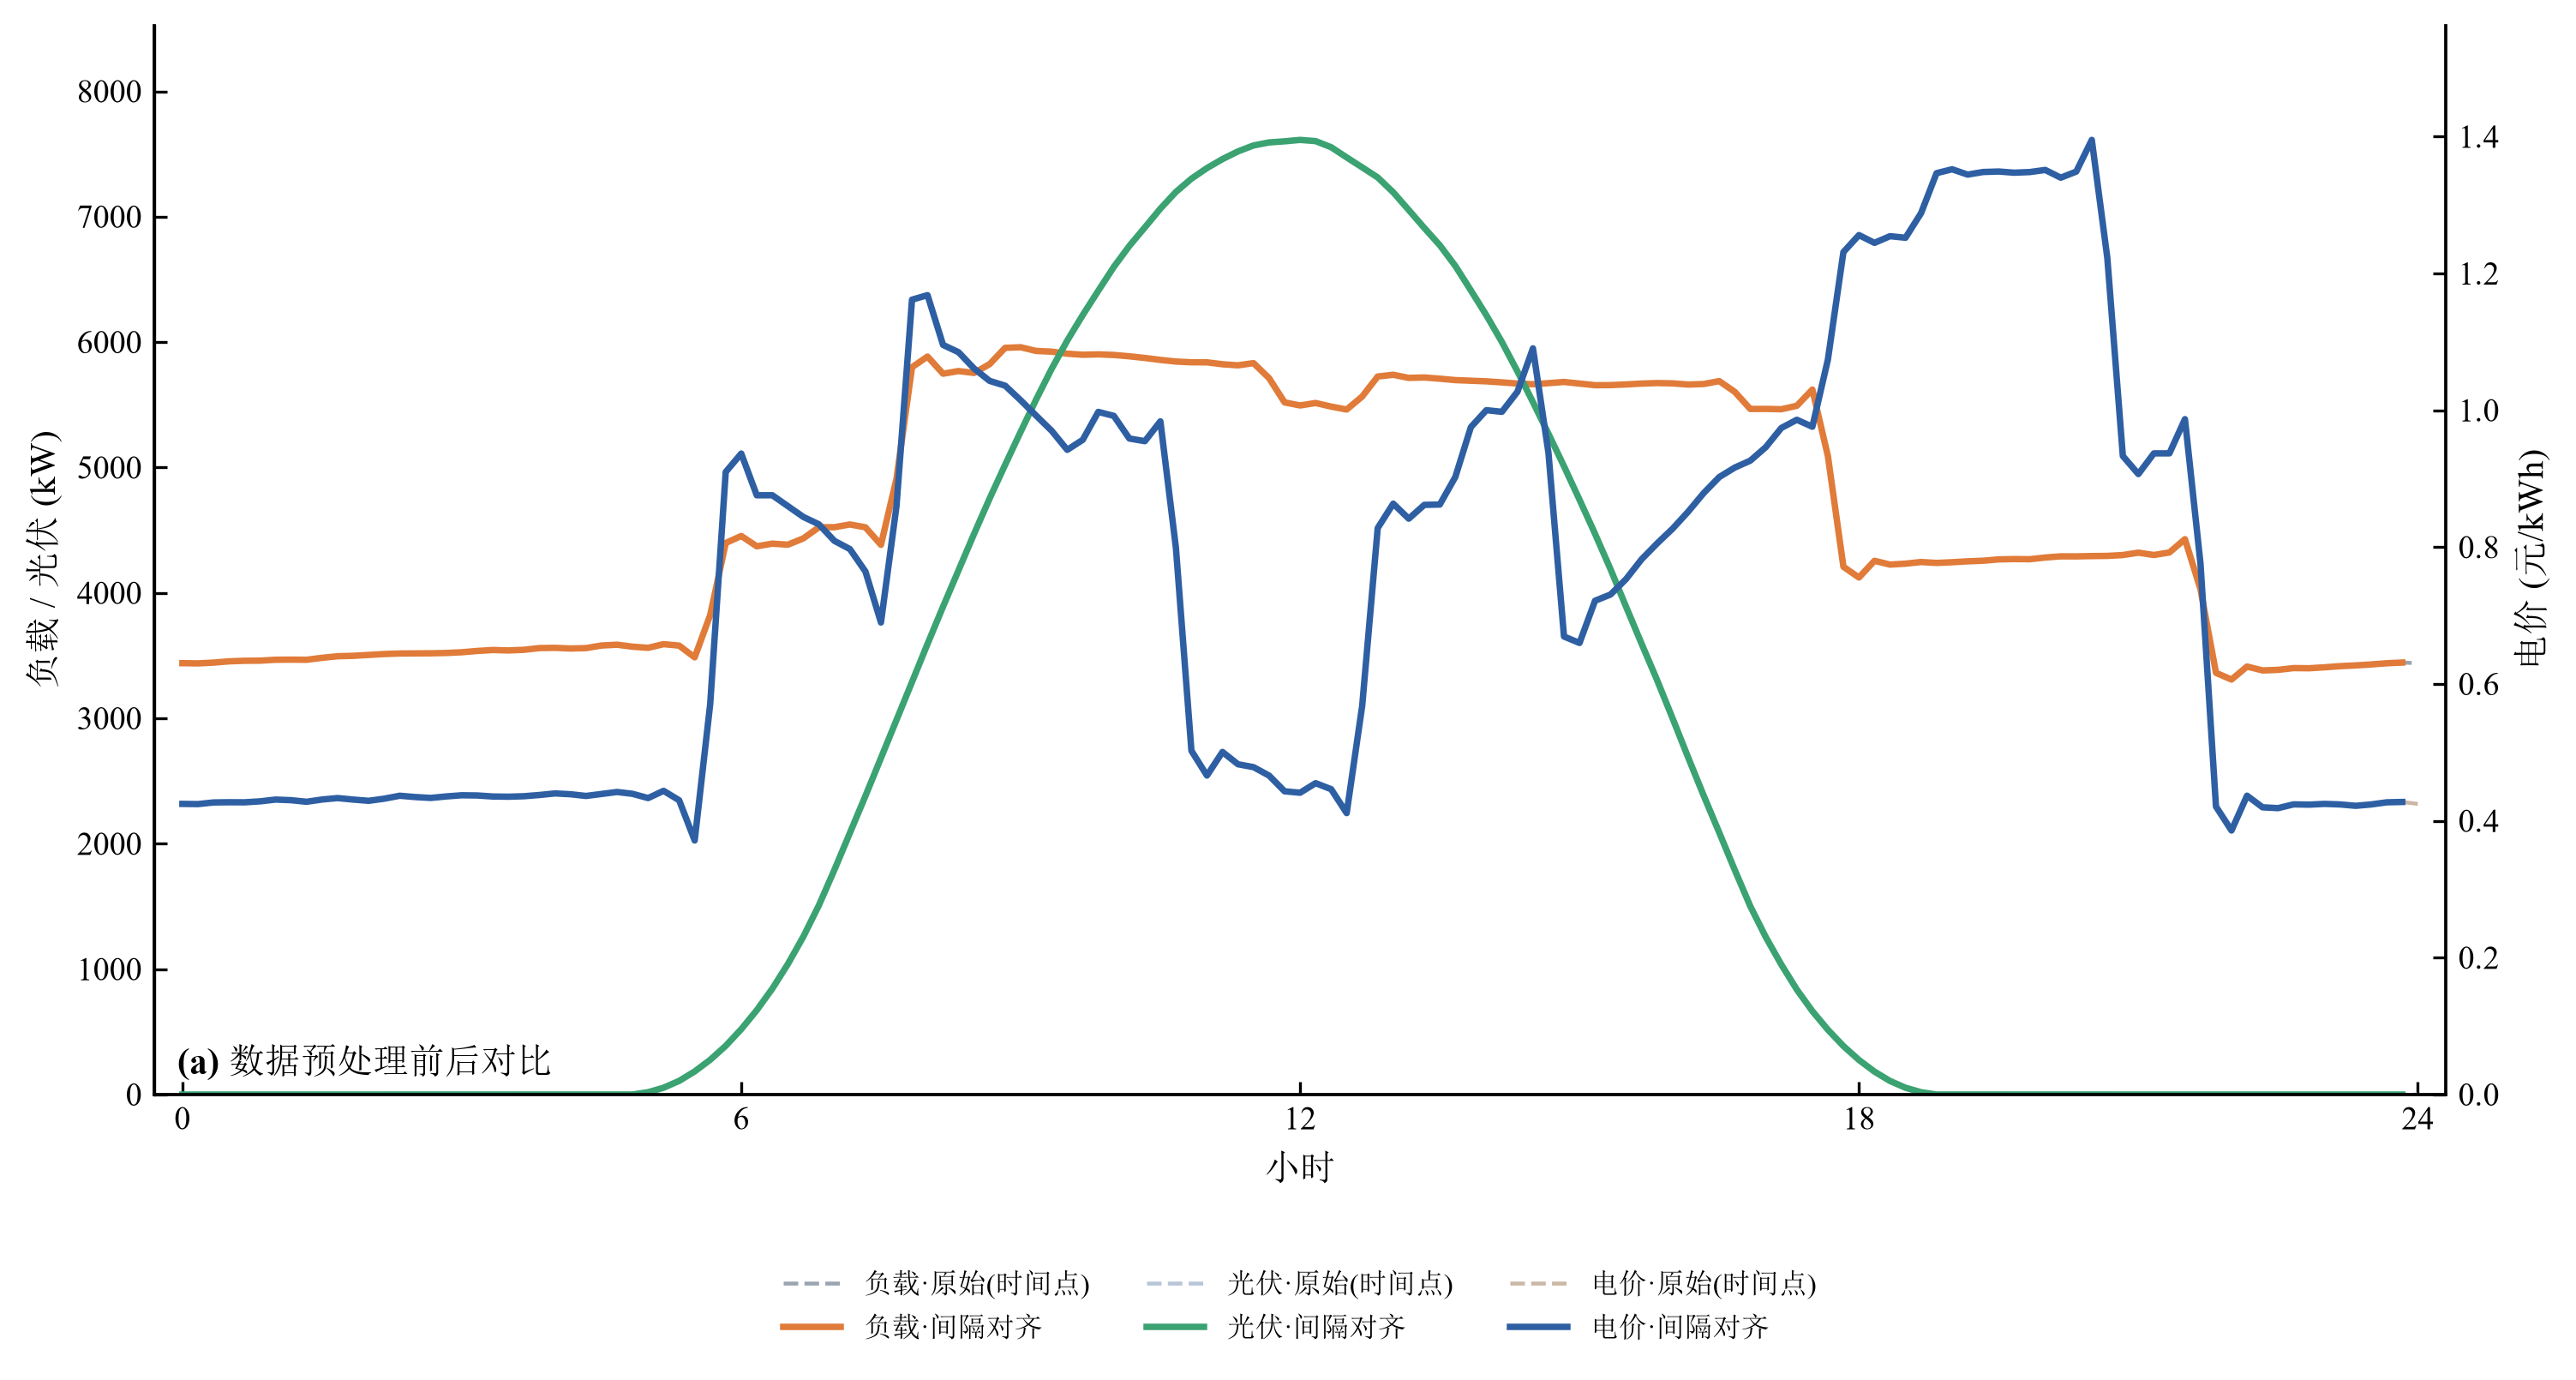
\includegraphics[width=0.72\textwidth]{求解/问题一/图片/图1-1_预处理前后对比.png}
    \caption{问题一数据预处理前后对比}
    \label{fig:preprocess1}
\end{figure}

由图\ref{fig:preprocess1}可知，预处理后电价、负载与光伏三条曲线均被完整对齐到 144 个 10 分钟间隔上，数据无缺失、无异常，且光伏功率在日出后至日落前呈现典型的单峰形态，为后续优化提供了可靠的输入。

\textbf{2.算法选择}

在完成数据预处理后，本问需要在一组候选算法中确定购电与储能调度的求解方法。微网购电调度本质上是一个带线性约束的凸优化问题，可从求解精度、计算效率与全局最优性等维度比较枚举搜索、贪心算法和线性规划三种候选方法，如表\ref{tab:algo1}所示。

\begin{longtable}{>{\centering\arraybackslash}p{0.18\textwidth}>{\centering\arraybackslash}p{0.26\textwidth}>{\centering\arraybackslash}p{0.24\textwidth}>{\centering\arraybackslash}p{0.20\textwidth}}
  \caption{问题一算法对比}
  \label{tab:algo1} \\
  \toprule
  算法 & 全局最优性 & 计算效率 & 约束处理 \\
  \midrule
  \endfirsthead
  \caption{问题一算法对比（续）} \\
  \toprule
  算法 & 全局最优性 & 计算效率 & 约束处理 \\
  \midrule
  \endhead
  \bottomrule
  \endfoot
  枚举搜索 & 可保证 & 极低 & 一般 \\
  贪心算法 & 无保证 & 高 & 困难 \\
  线性规划 & 严格保证 & 高 & 直接建模 \\
\end{longtable}

如\ref{tab:algo1}所示，枚举搜索虽然理论上能找到最优解，但决策变量规模达数百个，计算量爆炸；贪心算法难以同时协调储能容量约束与日循环约束；而线性规划能够把所有线性约束与目标函数直接纳入模型，由单纯形法或内点法求得全局最优解\cite{si2009}，且求解速度极快。综合以上分析，本问选择线性规划算法进行求解。


% ════════════════════════════════════════════
% 模型建立（5.1.3.模型建立.tex，三级子块）
% ════════════════════════════════════════════
\subsubsection{模型建立}

针对问题一，本节将从能量平衡与储能状态递推的角度建立微网日购电计划的线性规划模型。具体过程如下。

\textbf{步骤1：决策变量与目标函数}

定义模型的决策变量。设第 $k$ 个间隔的购电功率为 $g_k$，储能充电功率为 $c_k$，放电功率为 $d_k$，储电量为 $E_k$，其中 $k=0,1,\dots,143$，$E_k$ 为第 $k$ 个间隔起始时刻的储电量。微网全天购电费用为目标函数，即各间隔购电能量与电价乘积之和：
\begin{equation}
    \min \; Z=\sum_{k=0}^{143} g_k\,p_k\,\Delta t
\end{equation}
其中，$g_k\geq 0$ 为购电功率，$p_k$ 为第 $k$ 个间隔的交易电价，$\Delta t$ 为时间步长。该目标函数线性地刻画了微网的经济诉求。

\textbf{步骤2：功率平衡约束}

微网在每个间隔内须满足小区负载的用电需求。由功率守恒，购电功率、光伏功率与储能放电功率之和须不低于负载功率与储能充电功率之和，即允许在光伏过剩时弃光：
\begin{equation}
    g_k + S_k + d_k - c_k \geq L_k,\quad k=0,1,\dots,143
\end{equation}
其中，$S_k$ 为光伏预测功率，$L_k$ 为小区负载功率，$c_k,d_k$ 分别为充、放电功率。由于光伏发电边际成本为零，最优解会自动优先消纳光伏，只有在光伏与储能放电不足时才从外网购电。

\textbf{步骤3：储能状态递推约束}

储能设备的荷电状态随充放电行为逐间隔更新。考虑到充、放电效率均为 $\eta$，充电时从外部吸收的能量只有 $\eta$ 倍存入电池，放电时向负荷释放单位能量需从电池取出 $1/\eta$ 倍能量，因此递推关系为：
\begin{equation}
    E_{k+1}=E_k+\eta\,c_k\,\Delta t-\frac{1}{\eta}\,d_k\,\Delta t,\quad k=0,1,\dots,143
\end{equation}
其中，$\eta=0.9$ 为储能充放电效率。储能设备须满足容量上下限约束：
\begin{equation}
    E_{\min}\leq E_k\leq E_{\max},\quad E_{\min}=1200,\; E_{\max}=10800
\end{equation}
同时充放电功率受储能变换器额定功率限制：
\begin{equation}
    0\leq c_k\leq P_{\max},\quad 0\leq d_k\leq P_{\max},\quad P_{\max}=5000
\end{equation}

\textbf{步骤4：储电初值与日循环约束}

附录1给定 2025 年 1 月 1 日 0:00 的储电量为 6000 kWh，故储能 0:00 储电量应固定为：
\begin{equation}
    E_0=6000
\end{equation}
同时，问题一要求储能设备在 0:00 与 24:00 的储电量相同，以保证相邻日策略的可重复性，故加入日循环约束：
\begin{equation}
    E_0=E_{144}
\end{equation}
综上所述，问题一的完整线性规划模型为：
\begin{equation}
    \min \; Z=\sum_{k=0}^{143} g_k\,p_k\,\Delta t
\end{equation}
\begin{equation}
    \mathrm{s.t.}\quad g_k+S_k+d_k-c_k\geq L_k
\end{equation}
\begin{equation}
    E_{k+1}=E_k+\eta\,c_k\,\Delta t-\frac{1}{\eta}\,d_k\,\Delta t
\end{equation}
\begin{equation}
    E_{\min}\leq E_k\leq E_{\max},\quad 0\leq c_k,d_k\leq P_{\max},\quad g_k\geq 0
\end{equation}
\begin{equation}
    E_0=6000,\quad E_0=E_{144}
\end{equation}
该模型共有 $4\times 144+1=577$ 个连续变量，其中 $E_0$ 由附录1固定为 6000 kWh；全部约束均为线性等式或不等式，属于标准的线性规划问题\cite{dantzig1963}，可用单纯形法或内点法精确求解，且所得解即全局最优解。

综上所述，本节完成了问题一优化模型的建立，得到了以全天购电费用最小为目标、以功率平衡与储能状态为约束的线性规划模型，接下来将基于此进行求解。


% ════════════════════════════════════════════
% 模型求解（5.1.4.模型求解.tex，三级子块）
% ════════════════════════════════════════════
\subsubsection{模型求解}

基于上述模型，本节利用附件一数据在 Python 环境下调用线性规划求解器进行求解。核心参数为 $\Delta t=1/6$ h、$\eta=0.9$、$E_{\min}=1200$ kWh、$E_{\max}=10800$ kWh、$P_{\max}=5000$ kW，并按附录1给定 $E_0=6000$ kWh。求解得到微网在指定时间段的购电量及全天购电量和购电费如表\ref{tab:结果1-1}所示，储能设备在指定时段的充放电量及储电量如表\ref{tab:结果1-2}所示。

分时电价与最优购电功率的对应关系如图\ref{fig:结果1-2}所示。可以看到，购电功率主要集中在夜间低电价时段，用于在低价区间补充负荷缺口并为储能充电；在电价高峰时段购电功率明显下降，说明储能放电有效替代了高价购电。

负荷、光伏、净负荷与储能充放电功率的时序关系如图\ref{fig:结果1-3}所示。可以看出，光伏功率在白天形成明显高峰，使净负荷在午间大幅下降甚至转负，此时储能吸收光伏盈余进行充电；而在夜间与傍晚负荷高峰，储能放电填补净负荷缺口，购电功率相应减小。

\begin{figure}[H]
    \centering
    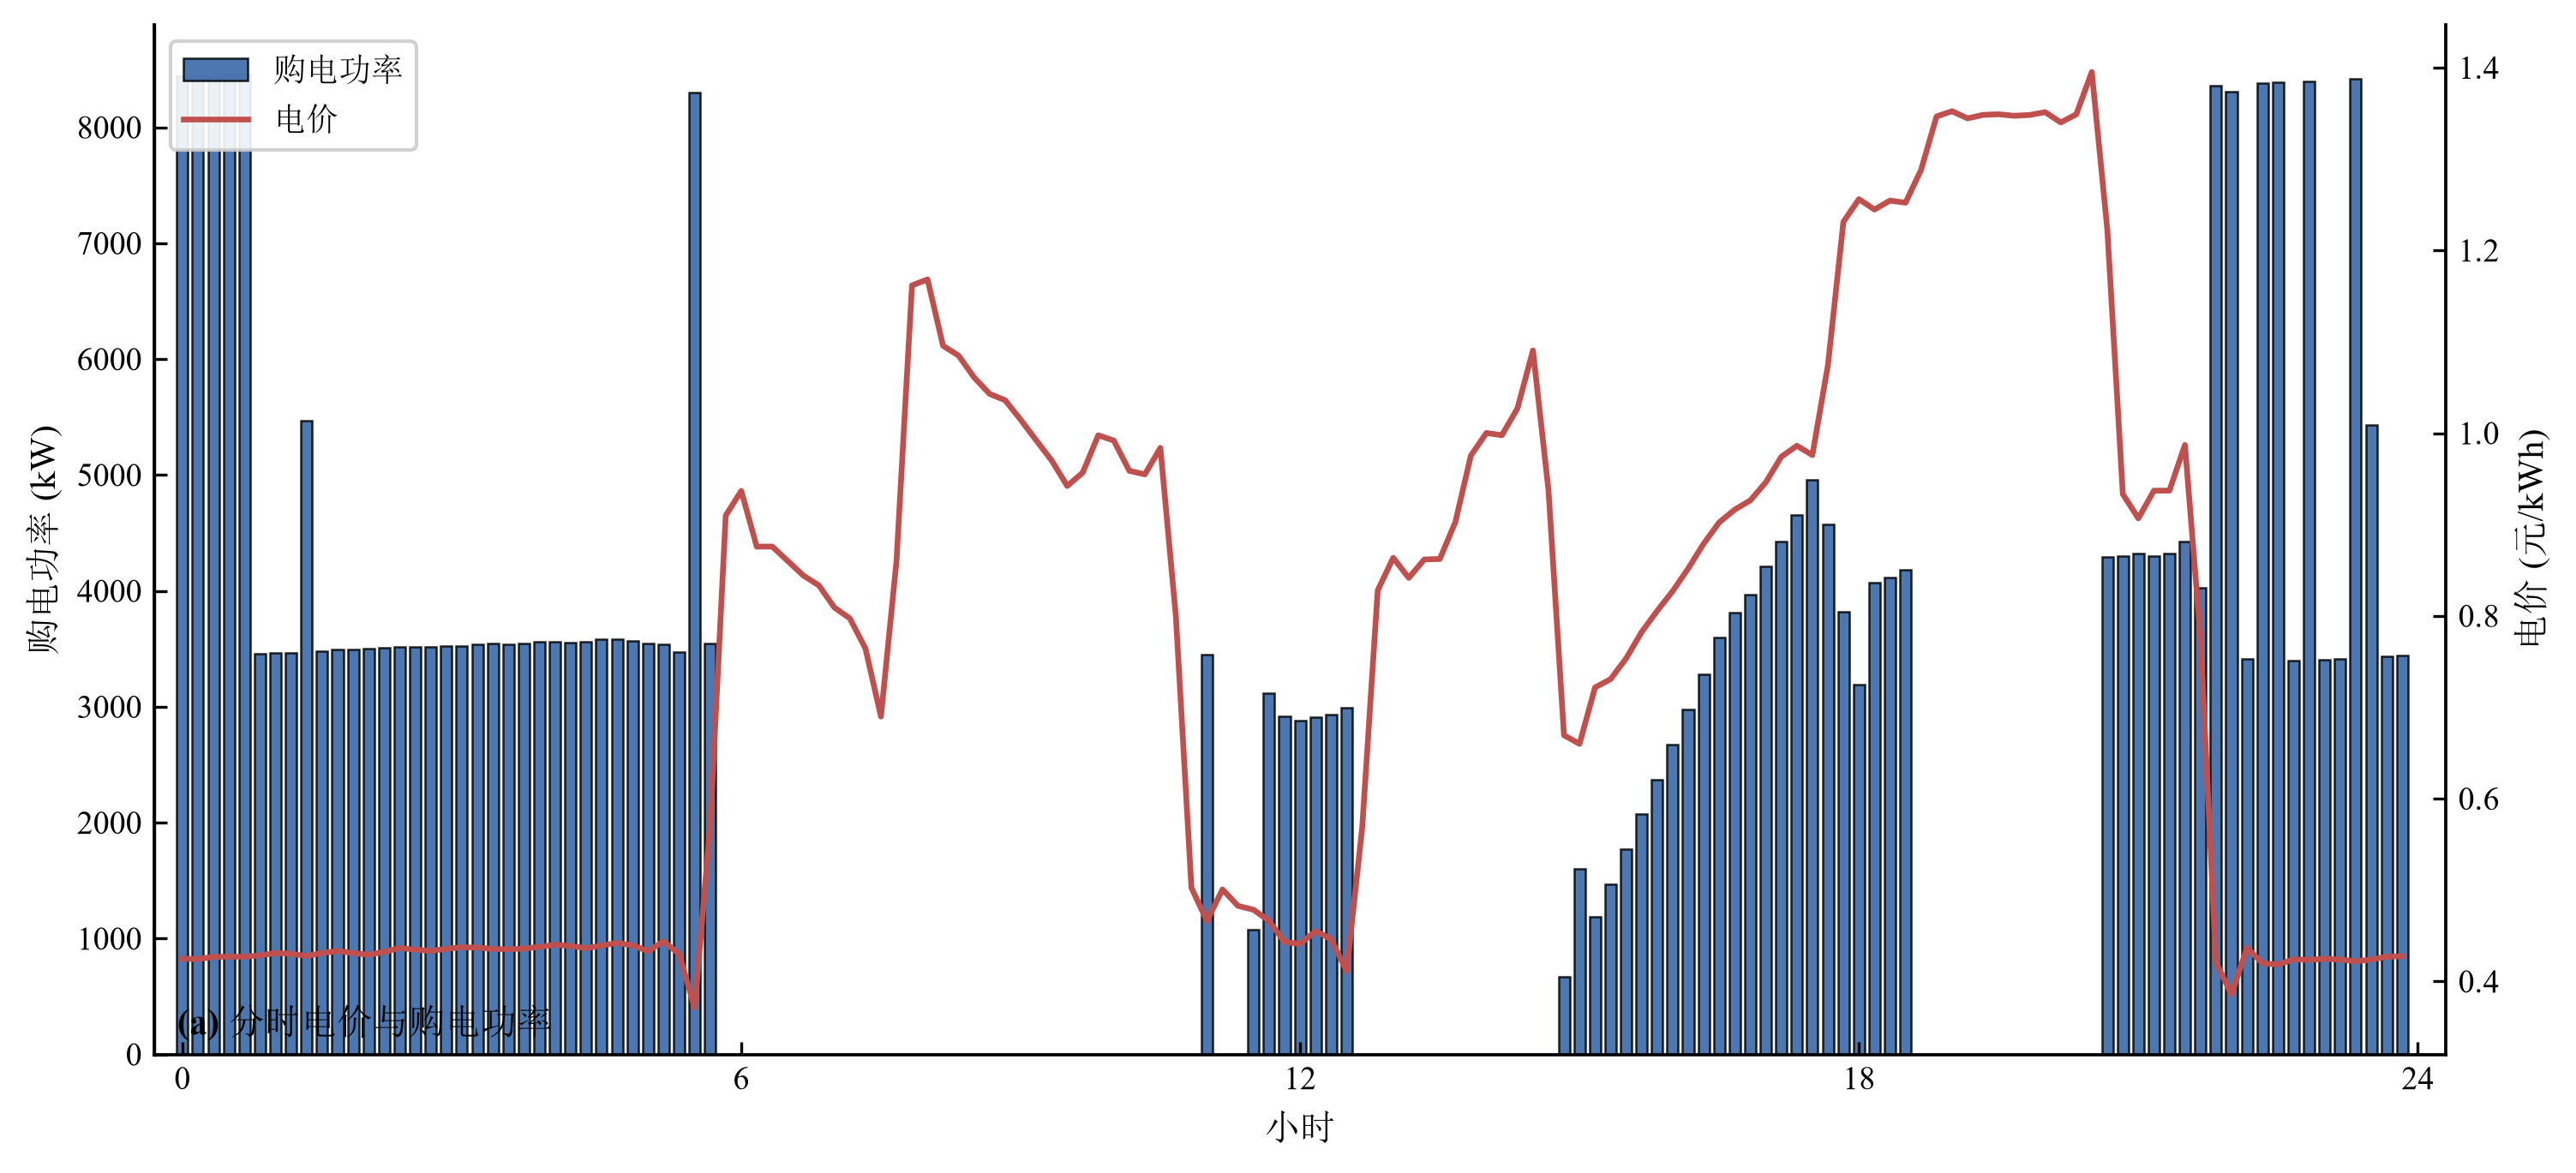
\includegraphics[width=0.65\textwidth]{求解/问题一/图片/图1-2_电价与购电策略.png}
    \caption{分时电价与最优购电功率}
    \label{fig:结果1-2}
\end{figure}

\begin{figure}[H]
    \centering
    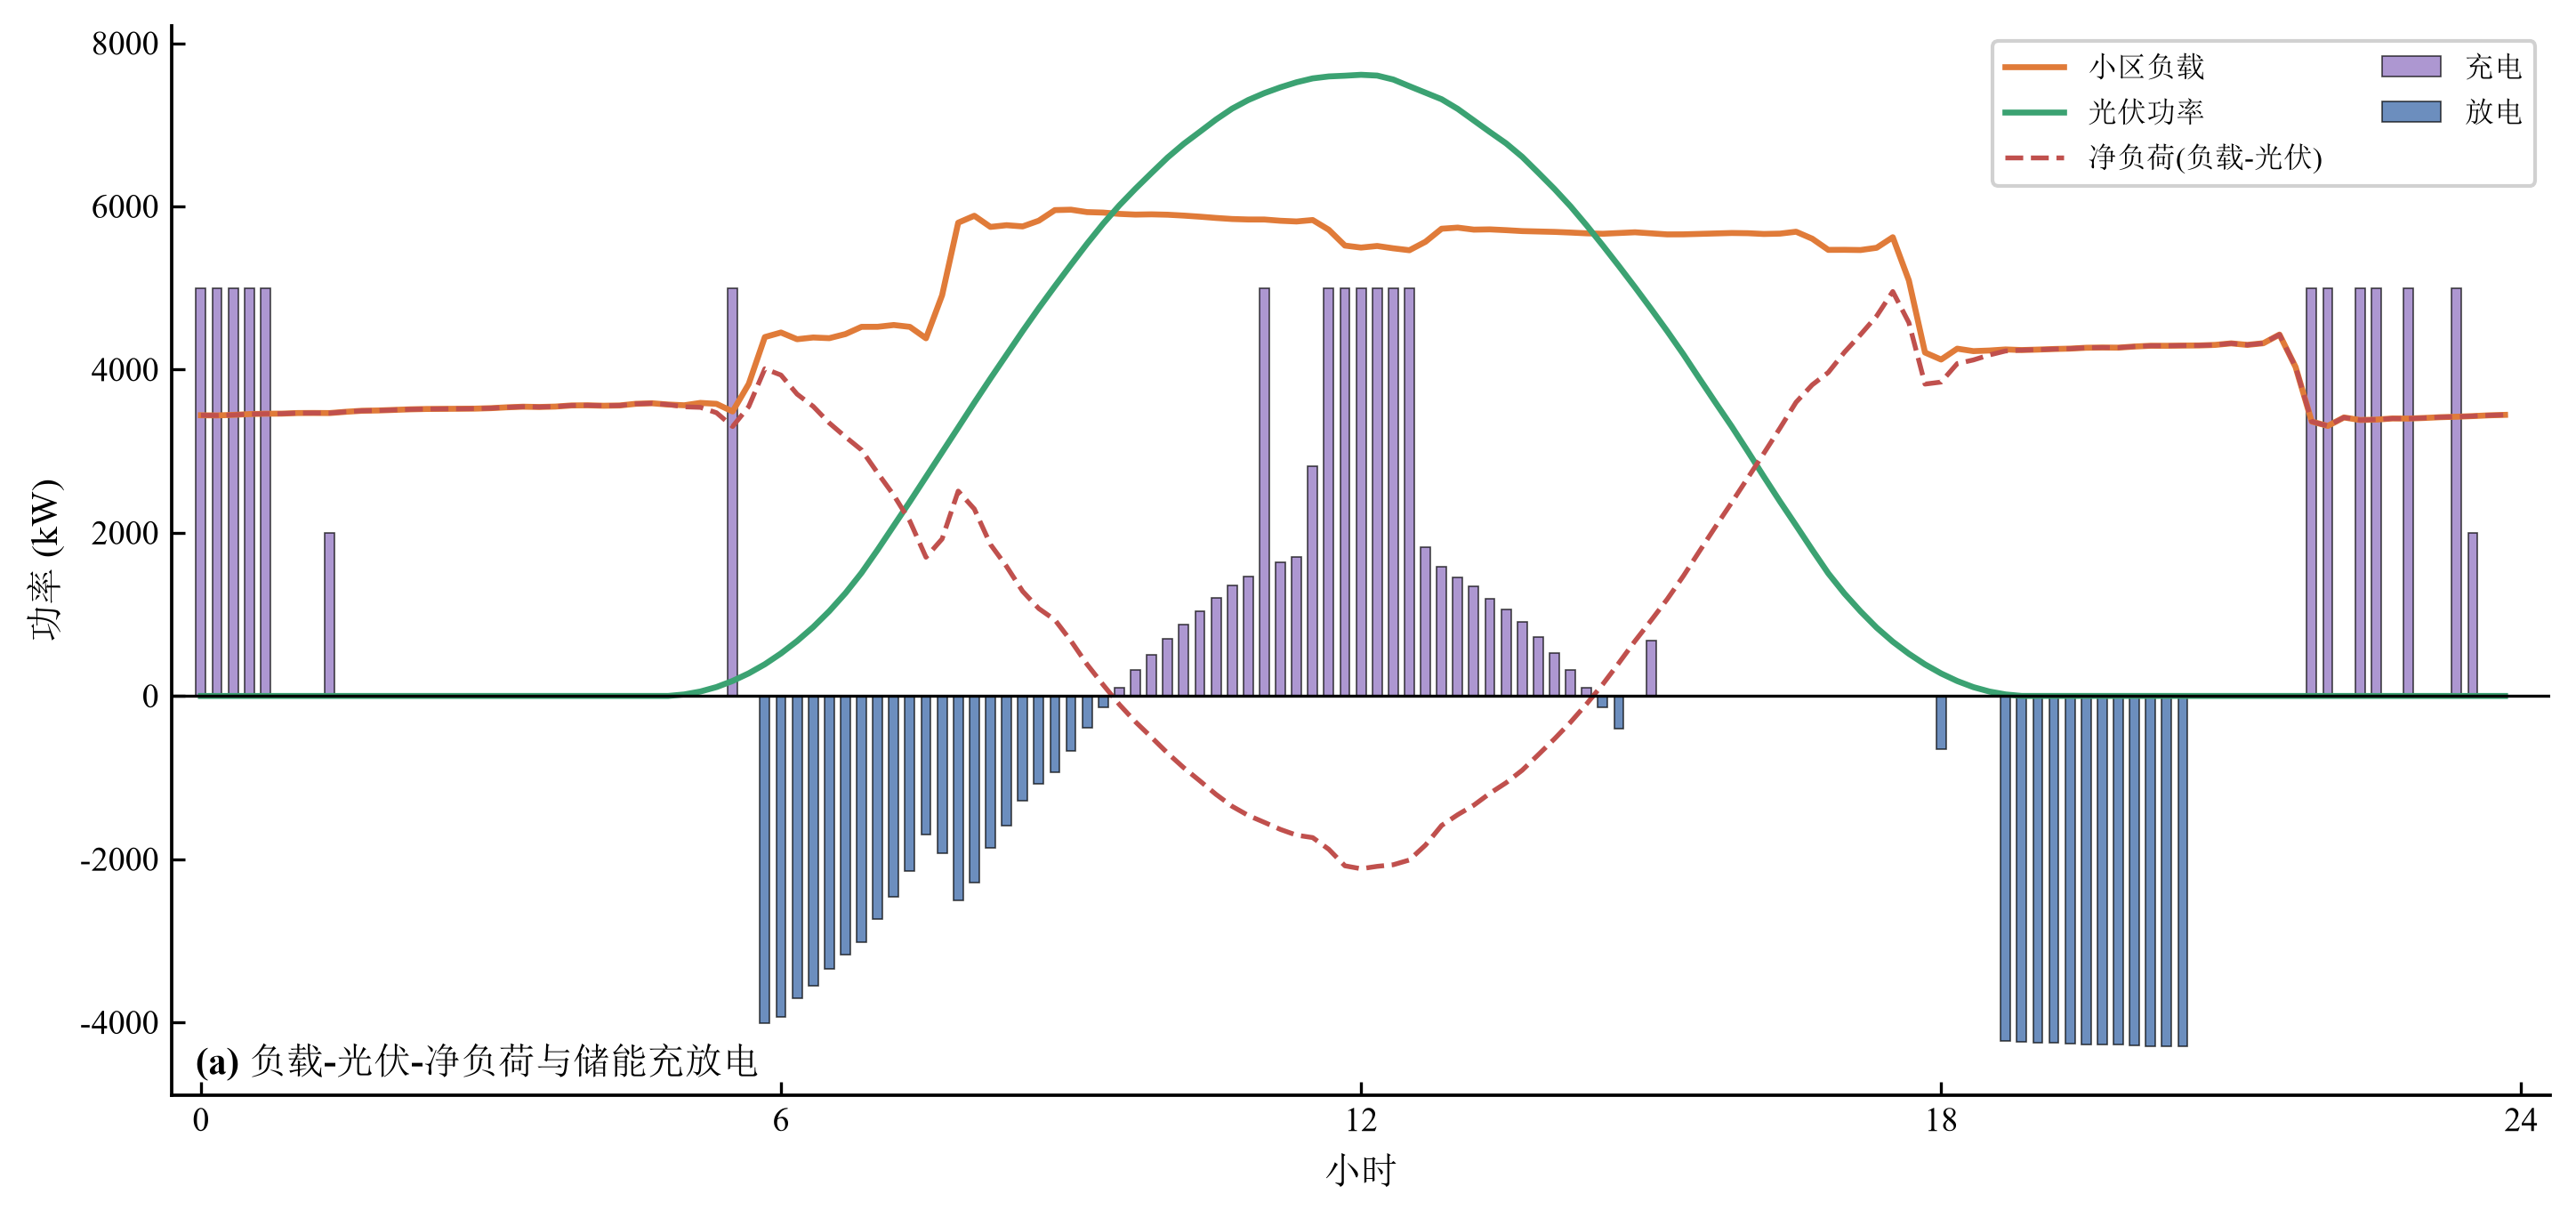
\includegraphics[width=0.65\textwidth]{求解/问题一/图片/图1-3_负荷光伏净负荷与充放电.png}
    \caption{负荷、光伏、净负荷与储能充放电功率}
    \label{fig:结果1-3}
\end{figure}

储能设备的荷电状态轨迹与充放电功率如图\ref{fig:结果1-4}所示。储能荷电状态全程维持在 $[1200,10800]$ kWh 约束区间内，且在 0:00 与 24:00 处均精确等于附录1给定的 6000 kWh；充放电功率始终不超过 5000 kW 的额定限值，验证了模型的可行性。

\begin{figure}[H]
    \centering
    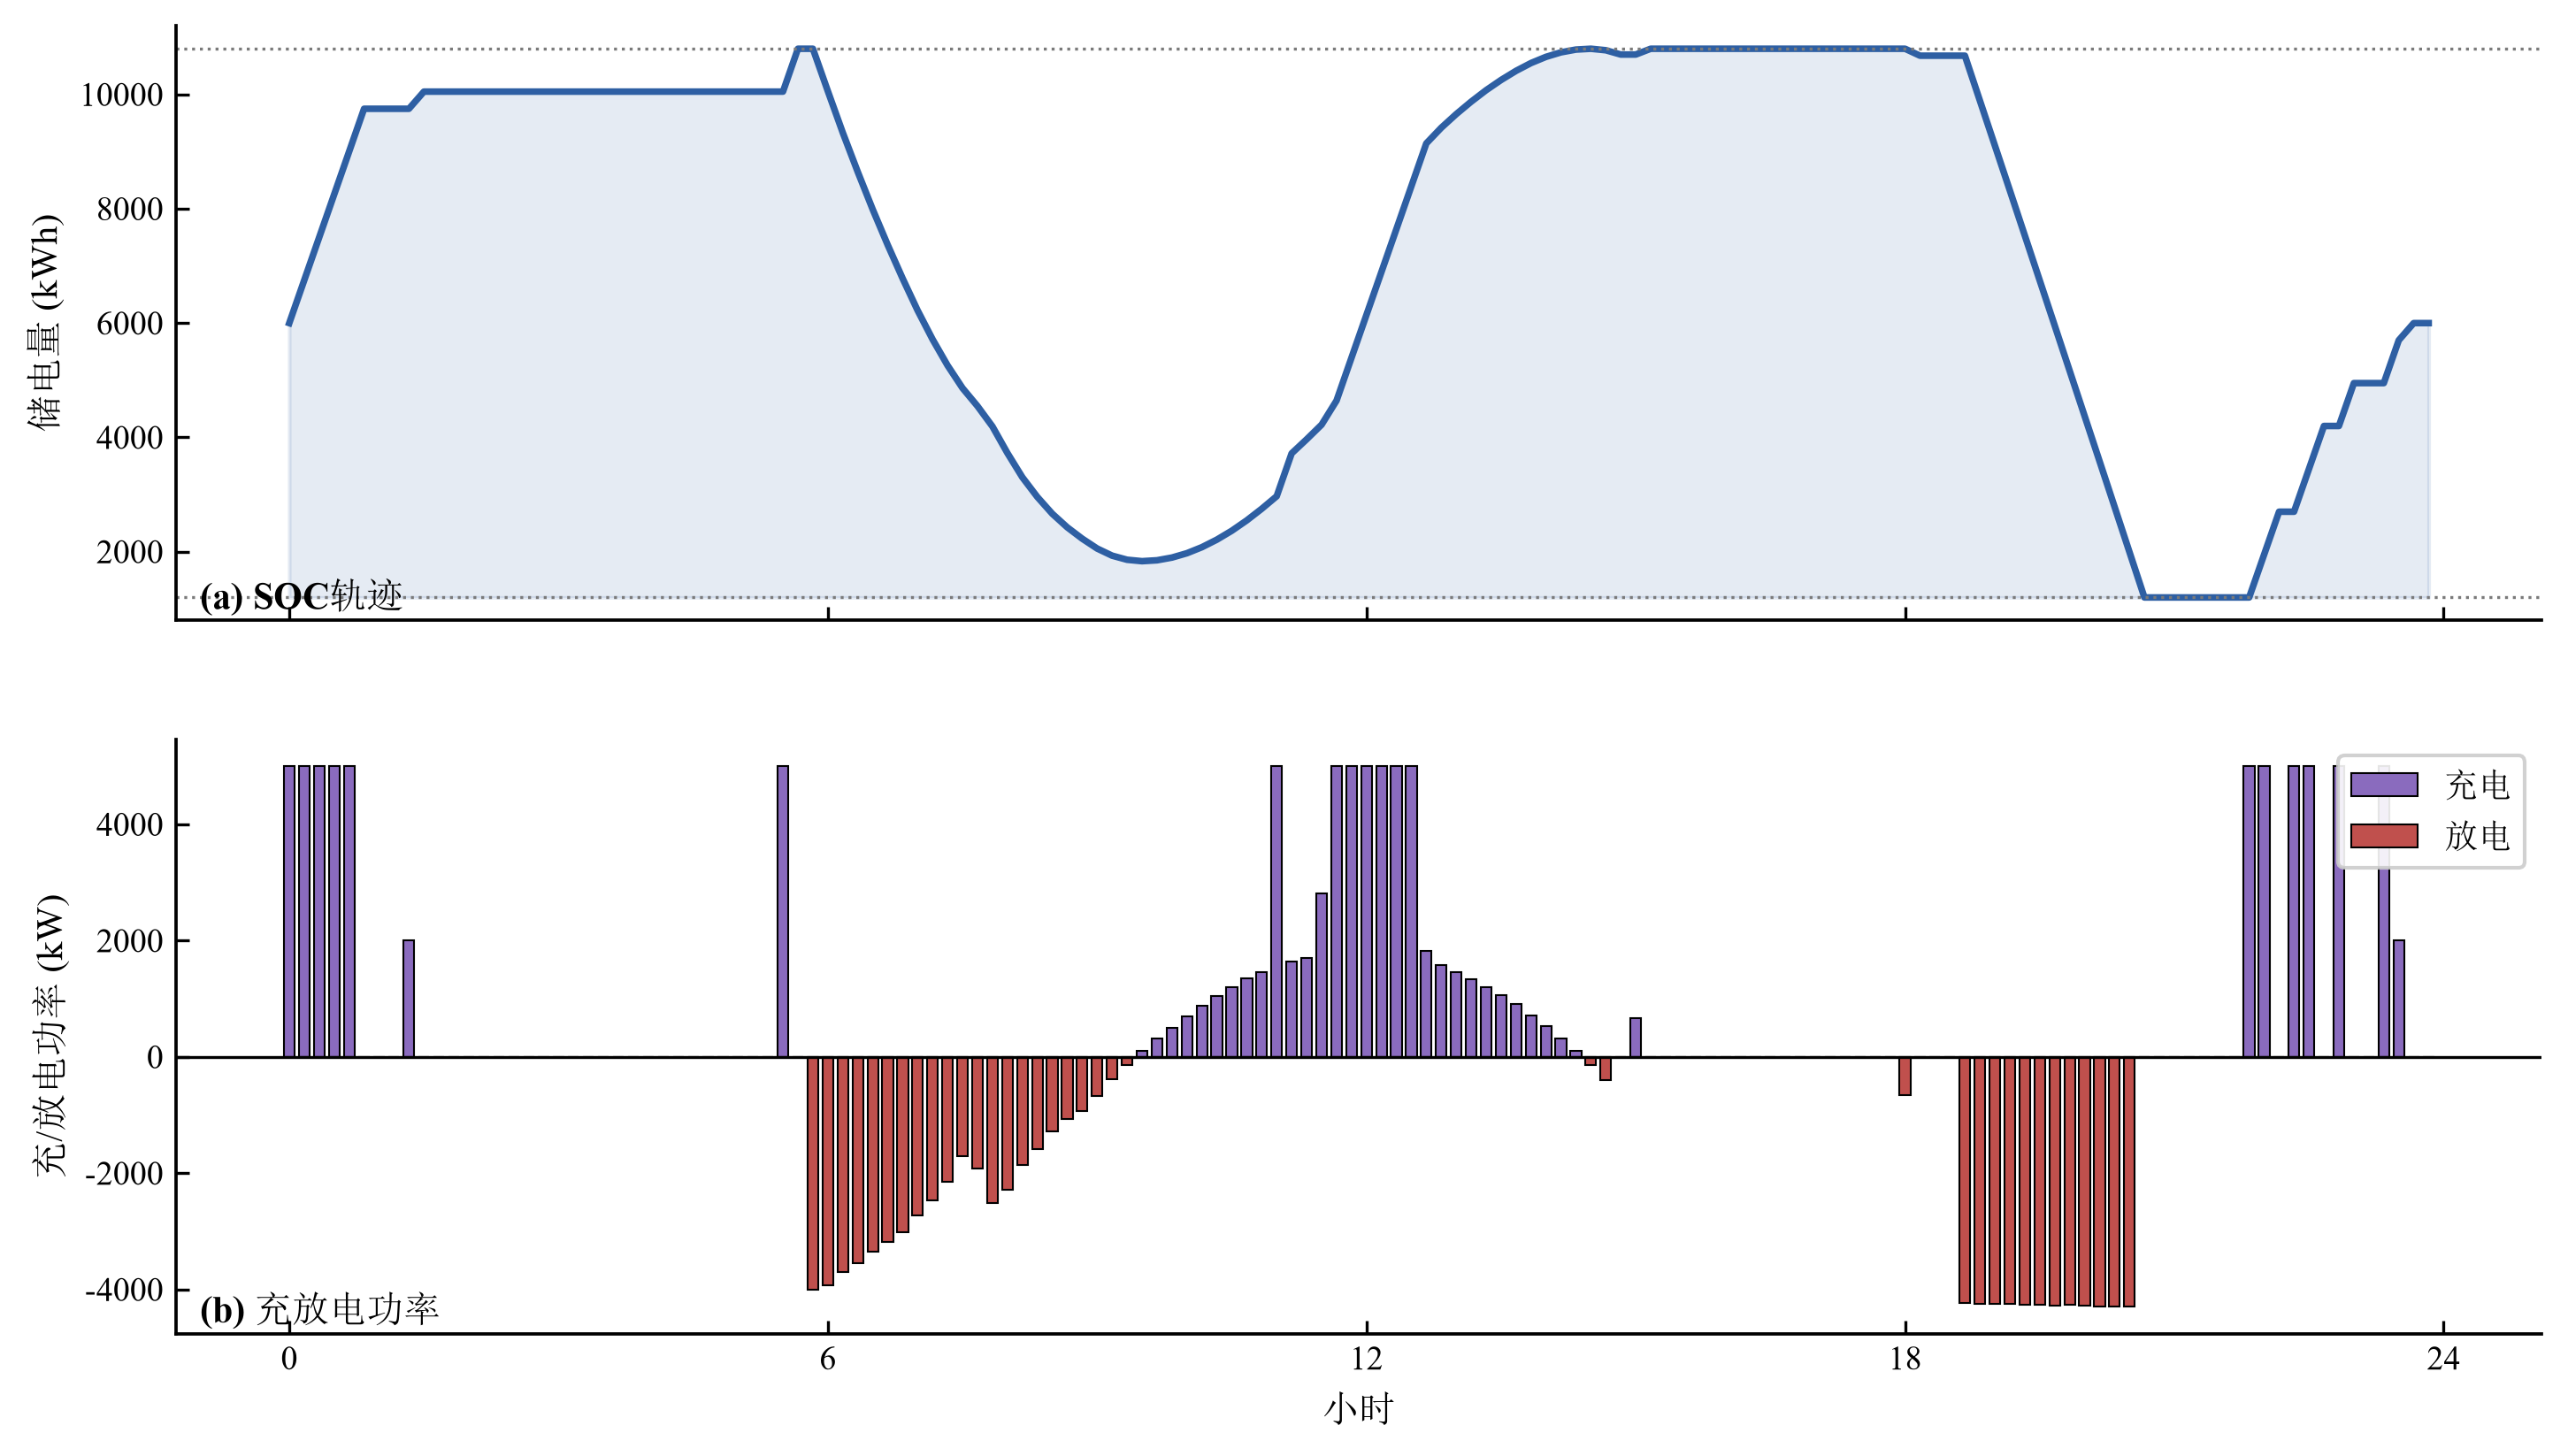
\includegraphics[width=0.62\textwidth]{求解/问题一/图片/图1-4_储能SOC与充放电功率.png}
    \caption{储能荷电状态轨迹与充放电功率}
    \label{fig:结果1-4}
\end{figure}

微网一天内的能量平衡关系如图\ref{fig:结果1-5}所示，购电、光伏与储能放电三类供给叠加后恰好覆盖小区负载与储能充电需求，任意时刻能量收支闭合，验证了功率平衡约束的严格满足。

\begin{figure}[H]
    \centering
    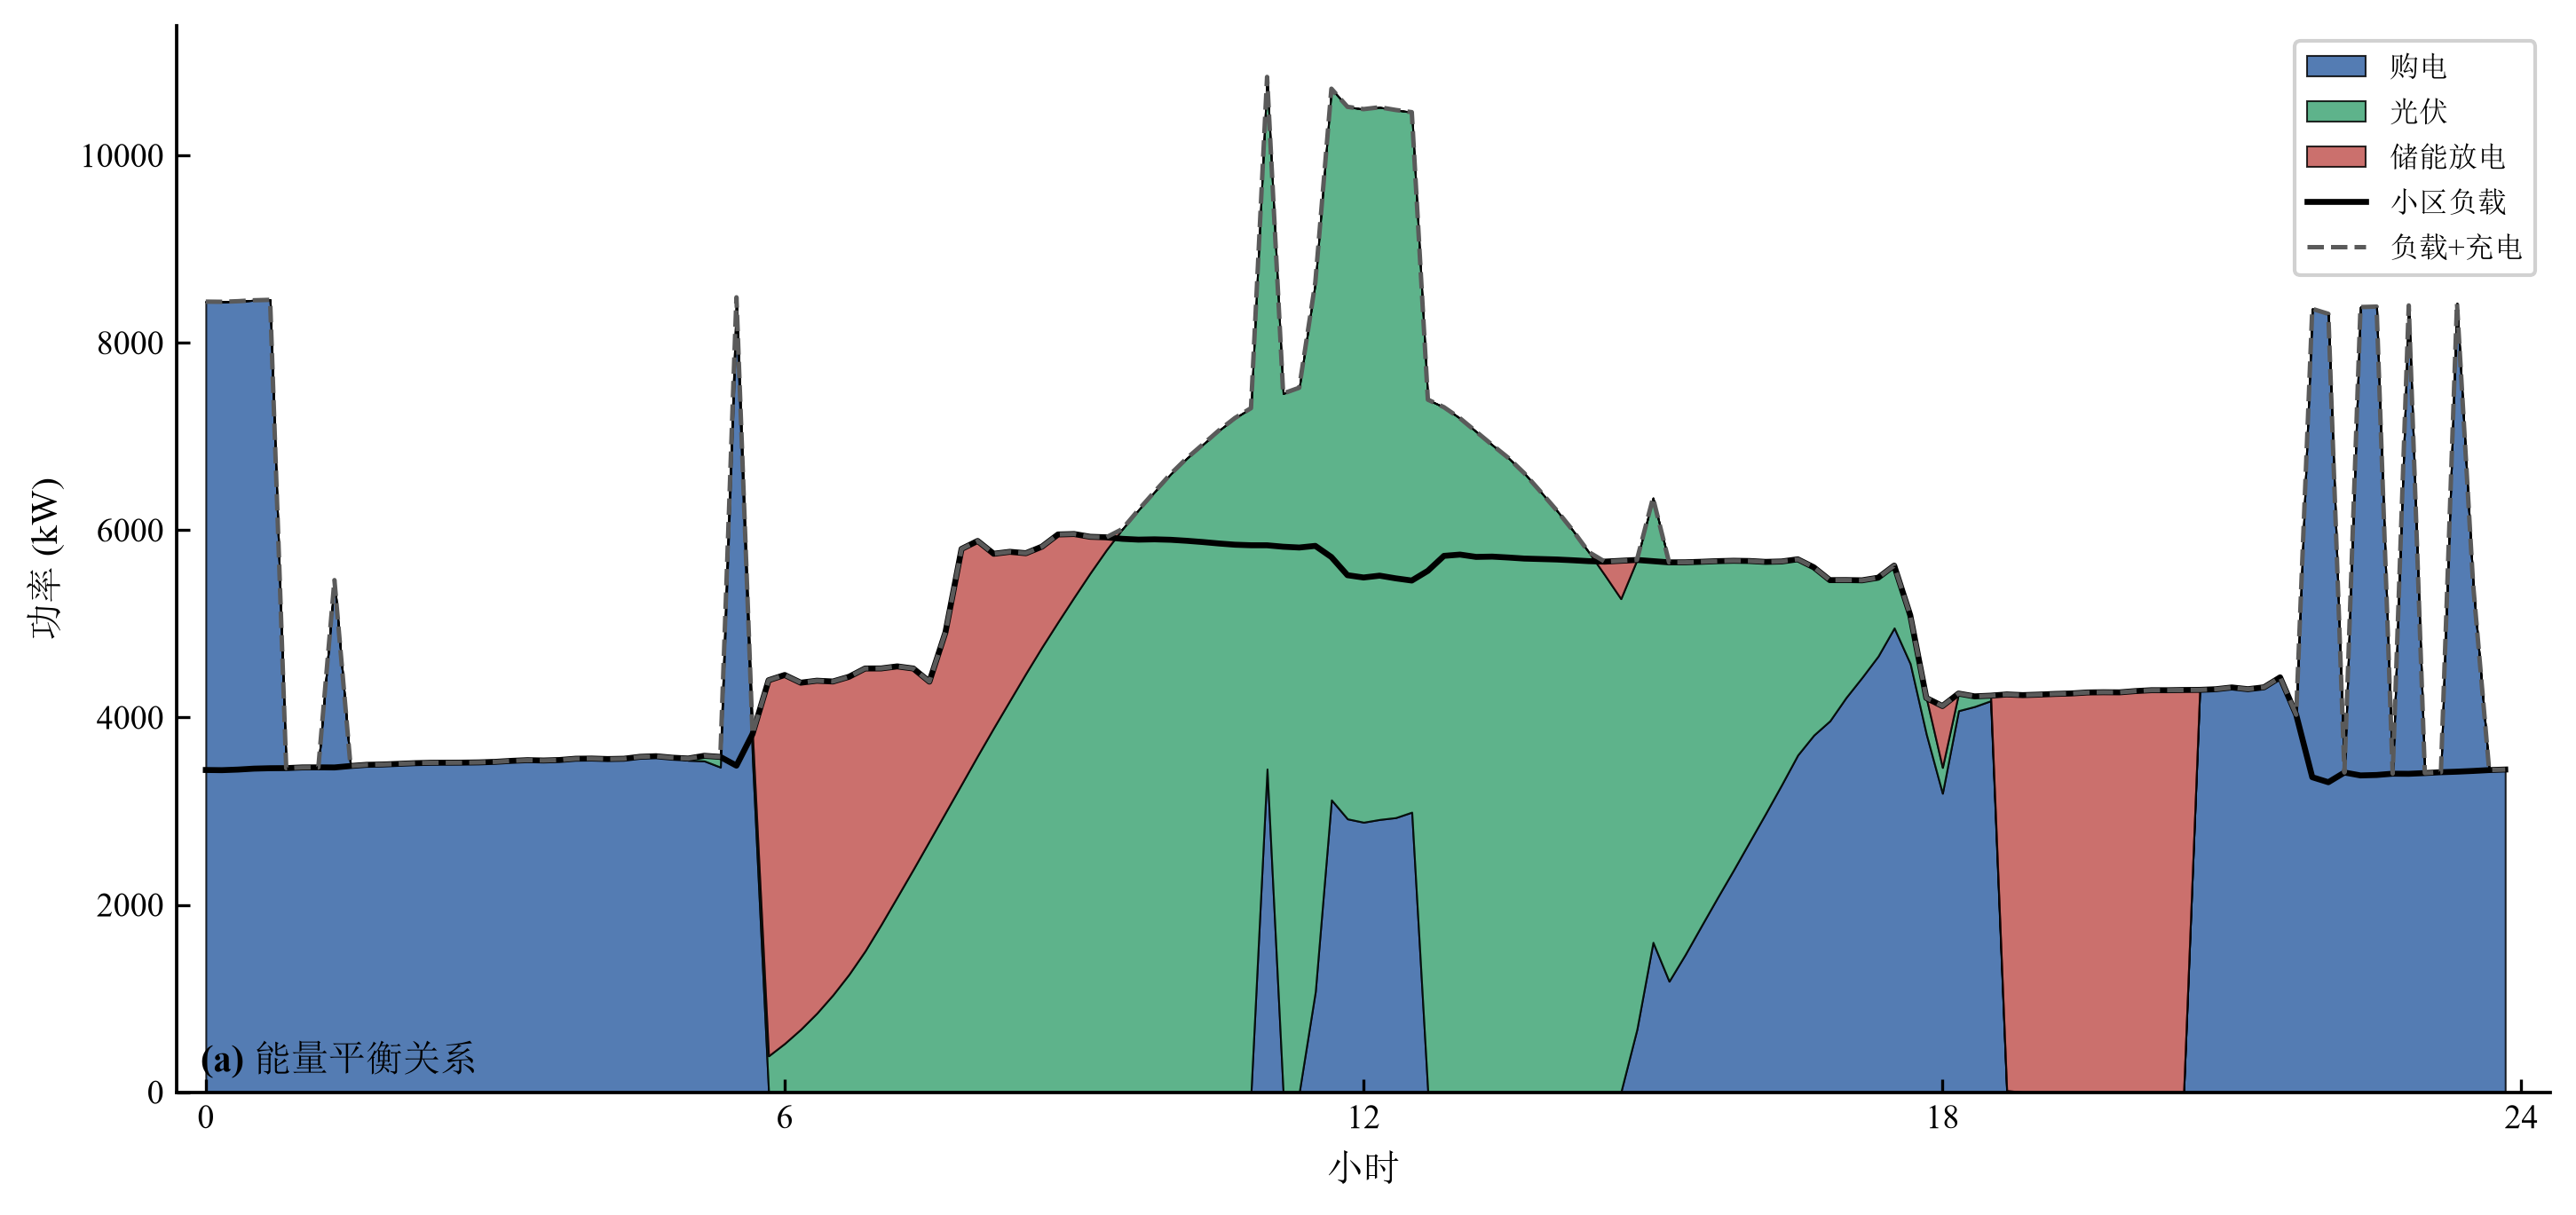
\includegraphics[width=0.70\textwidth]{求解/问题一/图片/图1-5_能量平衡.png}
    \caption{微网全天能量平衡关系}
    \label{fig:结果1-5}
\end{figure}

储能 0:00 储电量 $E_0$ 由附录1给定为 6000 kWh，属于问题给定的固定条件而非可优化变量。为进一步检验模型对该初值的稳健性，将 $E_0$ 在 $[1200,10800]$ kWh 区间内逐档变动（并保持日循环 $E_{144}=E_0$）重新求解全天购电费，结果如图\ref{fig:结果1-6}所示。可见购电费随 $E_0$ 变化总体平稳，在附录1给定的 6000 kWh 处购电费为 35126.95 元，与最低购电费相比差异很小，说明模型结果对储能初值的选取不敏感，也表明按给定初值求解是合理可靠的。

\begin{figure}[H]
    \centering
    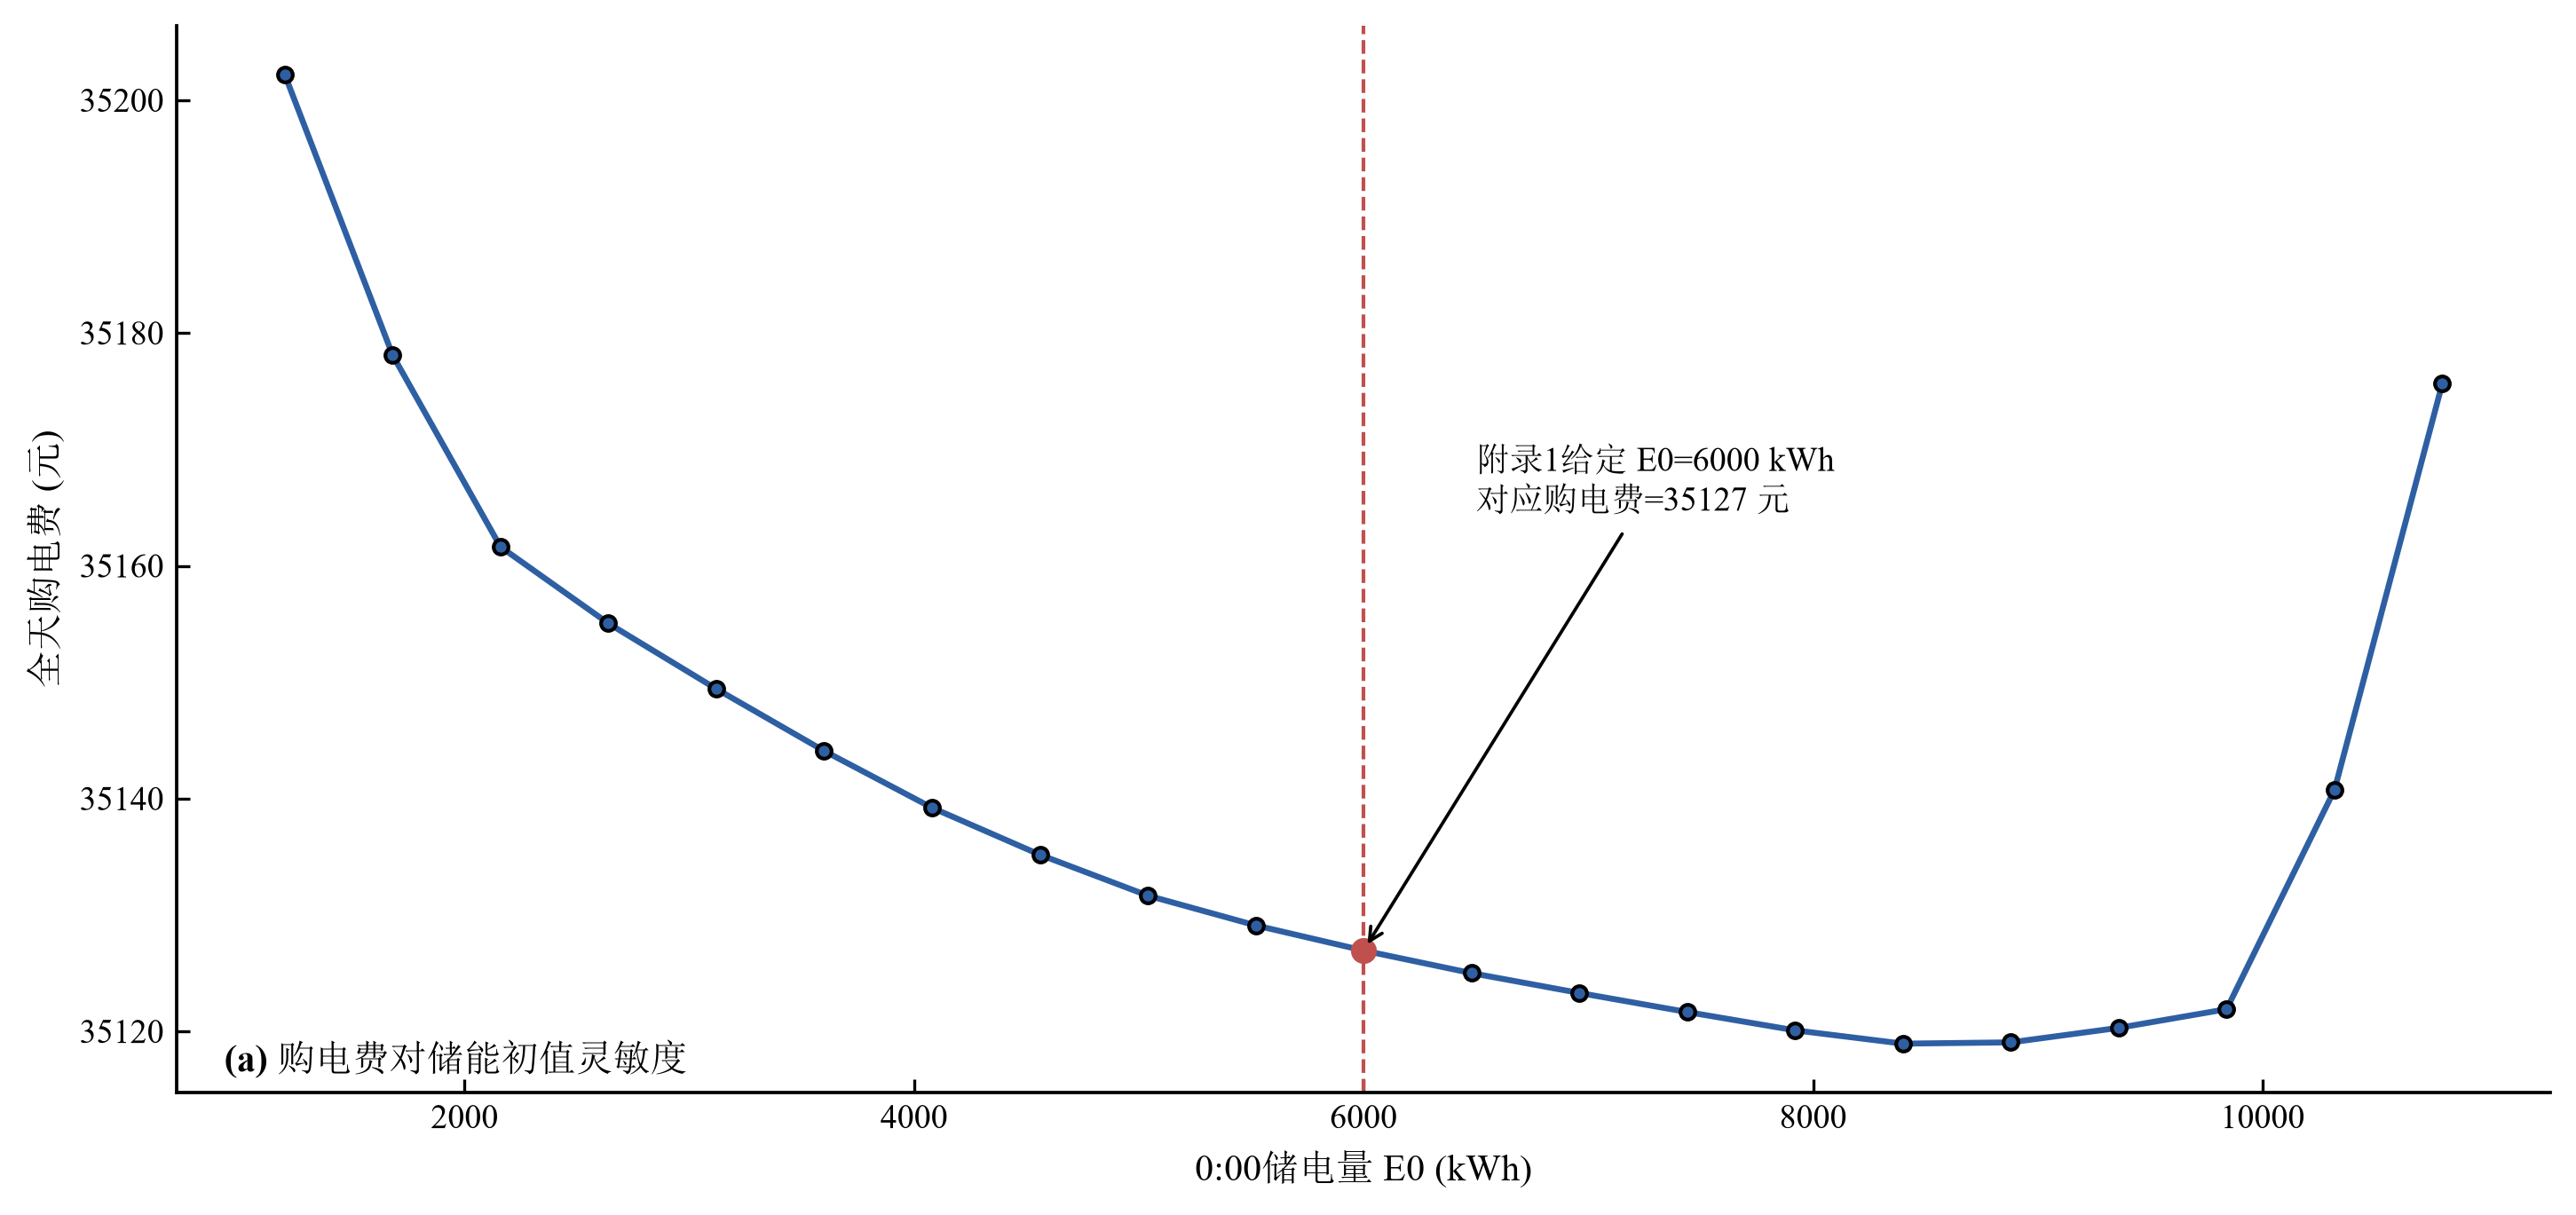
\includegraphics[width=0.70\textwidth]{求解/问题一/图片/图1-6_购电费灵敏度.png}
    \caption{全天购电费对储能初值的灵敏度}
    \label{fig:结果1-6}
\end{figure}

\begin{longtable}{>{\centering\arraybackslash}p{0.15\textwidth}>{\centering\arraybackslash}p{0.13\textwidth}>{\centering\arraybackslash}p{0.15\textwidth}>{\centering\arraybackslash}p{0.13\textwidth}>{\centering\arraybackslash}p{0.15\textwidth}>{\centering\arraybackslash}p{0.13\textwidth}}
  \caption{微网在指定时间段的购电量及全天的购电量和购电费}
  \label{tab:结果1-1} \\
  \toprule
  时间段 & 购电量 & 时间段 & 购电量 & 时间段 & 购电量 \\
  \midrule
  \endfirsthead
  \caption{微网在指定时间段的购电量及全天的购电量和购电费（续）} \\
  \toprule
  时间段 & 购电量 & 时间段 & 购电量 & 时间段 & 购电量 \\
  \midrule
  \endhead
  \bottomrule
  \endfoot
  10:00--10:10 & 0.00 & 12:00--12:10 & 480.41 & 14:00--14:10 & 0.00 \\
  16:00--16:10 & 445.43 & 18:00--18:10 & 531.89 & 20:00--20:10 & 0.00 \\
  全天购电量 & 59482.70 & 全天购电费 & 35126.95 &  &  \\
\end{longtable}

\begin{longtable}{>{\centering\arraybackslash}p{0.15\textwidth}>{\centering\arraybackslash}p{0.13\textwidth}>{\centering\arraybackslash}p{0.13\textwidth}>{\centering\arraybackslash}p{0.15\textwidth}>{\centering\arraybackslash}p{0.13\textwidth}>{\centering\arraybackslash}p{0.13\textwidth}}
  \caption{储能设备在指定时间段的充放电量及0:00和24:00的储电量}
  \label{tab:结果1-2} \\
  \toprule
  时间段 & 充电量 & 放电量 & 时间段 & 充电量 & 放电量 \\
  \midrule
  \endfirsthead
  \caption{储能设备在指定时间段的充放电量及0:00和24:00的储电量（续）} \\
  \toprule
  时间段 & 充电量 & 放电量 & 时间段 & 充电量 & 放电量 \\
  \midrule
  \endhead
  \bottomrule
  \endfoot
  0:00--4:00 & 4500.00 & 0.00 & 4:00--8:00 & 833.33 & 6365.84 \\
  8:00--12:00 & 4787.96 & 1703.00 & 12:00--16:00 & 5286.04 & 91.10 \\
  16:00--20:00 & 0.00 & 5780.13 & 20:00--24:00 & 5333.33 & 2859.87 \\
  0:00储电量 & 6000.00 &  & 24:00储电量 & 6000.00 &  \\
\end{longtable}

由表\ref{tab:结果1-1}可知，微网全天计划购电量为 59482.70 kWh，全天购电费为 35126.95 元；在 10:00--10:10、14:00--14:10 与 20:00--20:10 等光伏充足或储能放电充足的时段购电量为零，而在 12:00--12:10、16:00--16:10、18:00--18:10 等负荷高企时段需要少量购电。由表\ref{tab:结果1-2}可知，储能设备在 0:00 与 24:00 的储电量均为 6000.00 kWh，与附录1给定的 0:00 储电量一致，同时满足日循环约束；储能主要在 0:00--4:00、8:00--12:00 与 20:00--24:00 等低电价时段充电，在 4:00--8:00、16:00--20:00 等高电价时段放电，体现了低充高放的套利规律。

综合以上结果，问题一的线性规划模型在满足负载供电与储能运行约束的前提下，给出了全天购电费用最小的购电与充放电策略，储能设备在低价充电、高价放电的套利过程中使购电费用显著降低，模型与结果均合理可靠。



% ┈┈┈┈┈┈┈┈┈┈┈┈┈┈┈┈┈┈┈┈┈┈┈┈┈┈┈┈┈┈┈┈┈┈┈
% 【本章节写作提示词】
% ════════════════════════════════════════════
% 【作用】这是每个小问的包装（二级标题）：题目有几个小问，就在 模型的建立与求解 组成里放几个 5.X 子块，
%   并为每个小问复制本块为 5.X.问题X的建立求解（X = 第几小问）。
% 【结构】固定 \subsection{问题X的模型的建立和求解}，内部由下方「__SUBS__ 占位」注入四个三级子块，顺序固定为：
%   ① 具体分析 → ② 模型准备 → ③ 模型建立 → ④ 模型求解（见各子块顶部注释，组合题型按题目主要类型选择）。
% 【来源】图片 求解/问题X/图片/xxx.png；数据 求解/问题X/结果/ 的 CSV。
% ════════════════════════════════════════════


% ════════════════════════════════════════════
% 单个问题的建立求解（5.2.问题二.tex，二级标题包装）
% ════════════════════════════════════════════
\subsection{问题二的模型的建立和求解}


% ════════════════════════════════════════════
% 具体分析（5.2.1.具体分析.tex，三级子块）
% ════════════════════════════════════════════
\subsubsection{具体分析}

针对问题二，本问属于带时间序列输入的确定性滚动优化类问题，在问题一线性规划模型的基础上，将单日扩展为全年 365 天逐日递推，并引入紧急购电惩罚机制。

本文先读取附件一中每日相同的分时电价与附件二中全年 365 天的实际负载与光伏功率数据，按天组织为 365 组 144 维功率序列；以附录一给定的 2025 年 1 月 1 日 0:00 储电量 6000 kWh 为起点，逐日求解线性规划（其中 1 月作为预热期），并将每日末储电量传递给次日作为初值；针对实际供电低于负载的情形建立紧急购电费用项，其电价为交易时刻电价的 5 倍；最后输出 2025 年 2 月 1 日至 12 月 31 日共 334 天的计划购电量、储能充放电量与紧急购电量。具体分析流程如图\ref{fig:analysis2_flow}所示。

\begin{figure}[H]
    \begin{center}
        \begin{tikzpicture}[x=1cm, y=0.75cm,
            flowhead/.style={rectangle, rounded corners=3pt, draw=green!60!black, fill=green!45!black, text=white, font=\bfseries, minimum width=7.2cm, minimum height=1.1cm, align=center, inner sep=2pt, line width=0.7pt},
            flowbox/.style={rectangle, rounded corners=2.5pt, draw=green!55!black, fill=green!12, minimum width=7.2cm, minimum height=1.0cm, align=center, inner sep=2pt, line width=0.6pt},
            flowend/.style={rectangle, rounded corners=2.5pt, draw=green!65!black, fill=green!35!black, text=white, font=\bfseries, minimum width=7.2cm, minimum height=1.0cm, align=center, inner sep=2pt, line width=0.7pt},
            flowarrow/.style={thick, -{Stealth}, green!50!black}
        ]
            \node[flowhead] at (0, 0) (h) {问题二：全年逐日滚动优化};
            \node[flowbox] at (0, -1.8) (s1) {\textbf{读取全年数据}\\\footnotesize 365 天负荷 · 光伏 · 分时电价};
            \node[flowbox] at (0, -3.6) (s2) {\textbf{按天切分对齐}\\\footnotesize 365 组 144 维功率序列};
            \node[flowbox] at (0, -5.4) (s3) {\textbf{设定储电初值}\\\footnotesize 1 月 1 日 0:00 储电量 6000 kWh};
            \node[flowbox] at (0, -7.2) (s4) {\textbf{逐日线性规划}\\\footnotesize 单日购电与充放电联合优化};
            \node[flowbox] at (0, -9.0) (s5) {\textbf{日间储电量传递}\\\footnotesize 当日末储电量作为次日初值};
            \node[flowbox] at (0, -10.8) (s6) {\textbf{紧急购电惩罚}\\\footnotesize 按交易电价 5 倍计价};
            \node[flowbox] at (0, -12.6) (s7) {\textbf{滚动递推全年}\\\footnotesize 逐日递推共 365 天};
            \node[flowend] at (0, -14.4) (s8) {汇总输出结果\\\footnotesize 2 月 1 日—12 月 31 日购电与紧急购电量};
            \draw[flowarrow] (h) -- (s1);
            \draw[flowarrow] (s1) -- (s2);
            \draw[flowarrow] (s2) -- (s3);
            \draw[flowarrow] (s3) -- (s4);
            \draw[flowarrow] (s4) -- (s5);
            \draw[flowarrow] (s5) -- (s6);
            \draw[flowarrow] (s6) -- (s7);
            \draw[flowarrow] (s7) -- (s8);
        \end{tikzpicture}
        \caption{问题二分析流程图}
        \label{fig:analysis2_flow}
    \end{center}
\end{figure}


% ════════════════════════════════════════════
% 模型准备（5.2.2.模型准备.tex，三级子块）
% ════════════════════════════════════════════
\subsubsection{模型准备}

\textbf{1.数据预处理}

附件二提供了 2025 年全年 365 天、每天 144 个 10 分钟时间点的小区负载与光伏实际功率数据，数据量约为 $365\times 144$ 的两张二维矩阵。为便于逐日建模，需要对数据进行时间对齐、数值化与按天切分。设第 $d$ 天第 $k$ 个间隔的负载与光伏功率分别为 $L_{d,k}$ 与 $S_{d,k}$，则全年数据可组织为：
\begin{equation}
    \boldsymbol{L}=[L_{d,k}]_{365\times 144},\quad \boldsymbol{S}=[S_{d,k}]_{365\times 144}
\end{equation}
其中，$d=0,1,\dots,364$ 表示天数序号，$k$ 表示日内间隔序号。对两张矩阵逐元素执行数值化检查，全年缺失值为零，负载分布于 $1995.7\sim 7978.9$ kW，光伏分布于 $0\sim 10216.2$ kW。预处理前后对比如图\ref{fig:preprocess2}所示。

\begin{figure}[H]
    \centering
    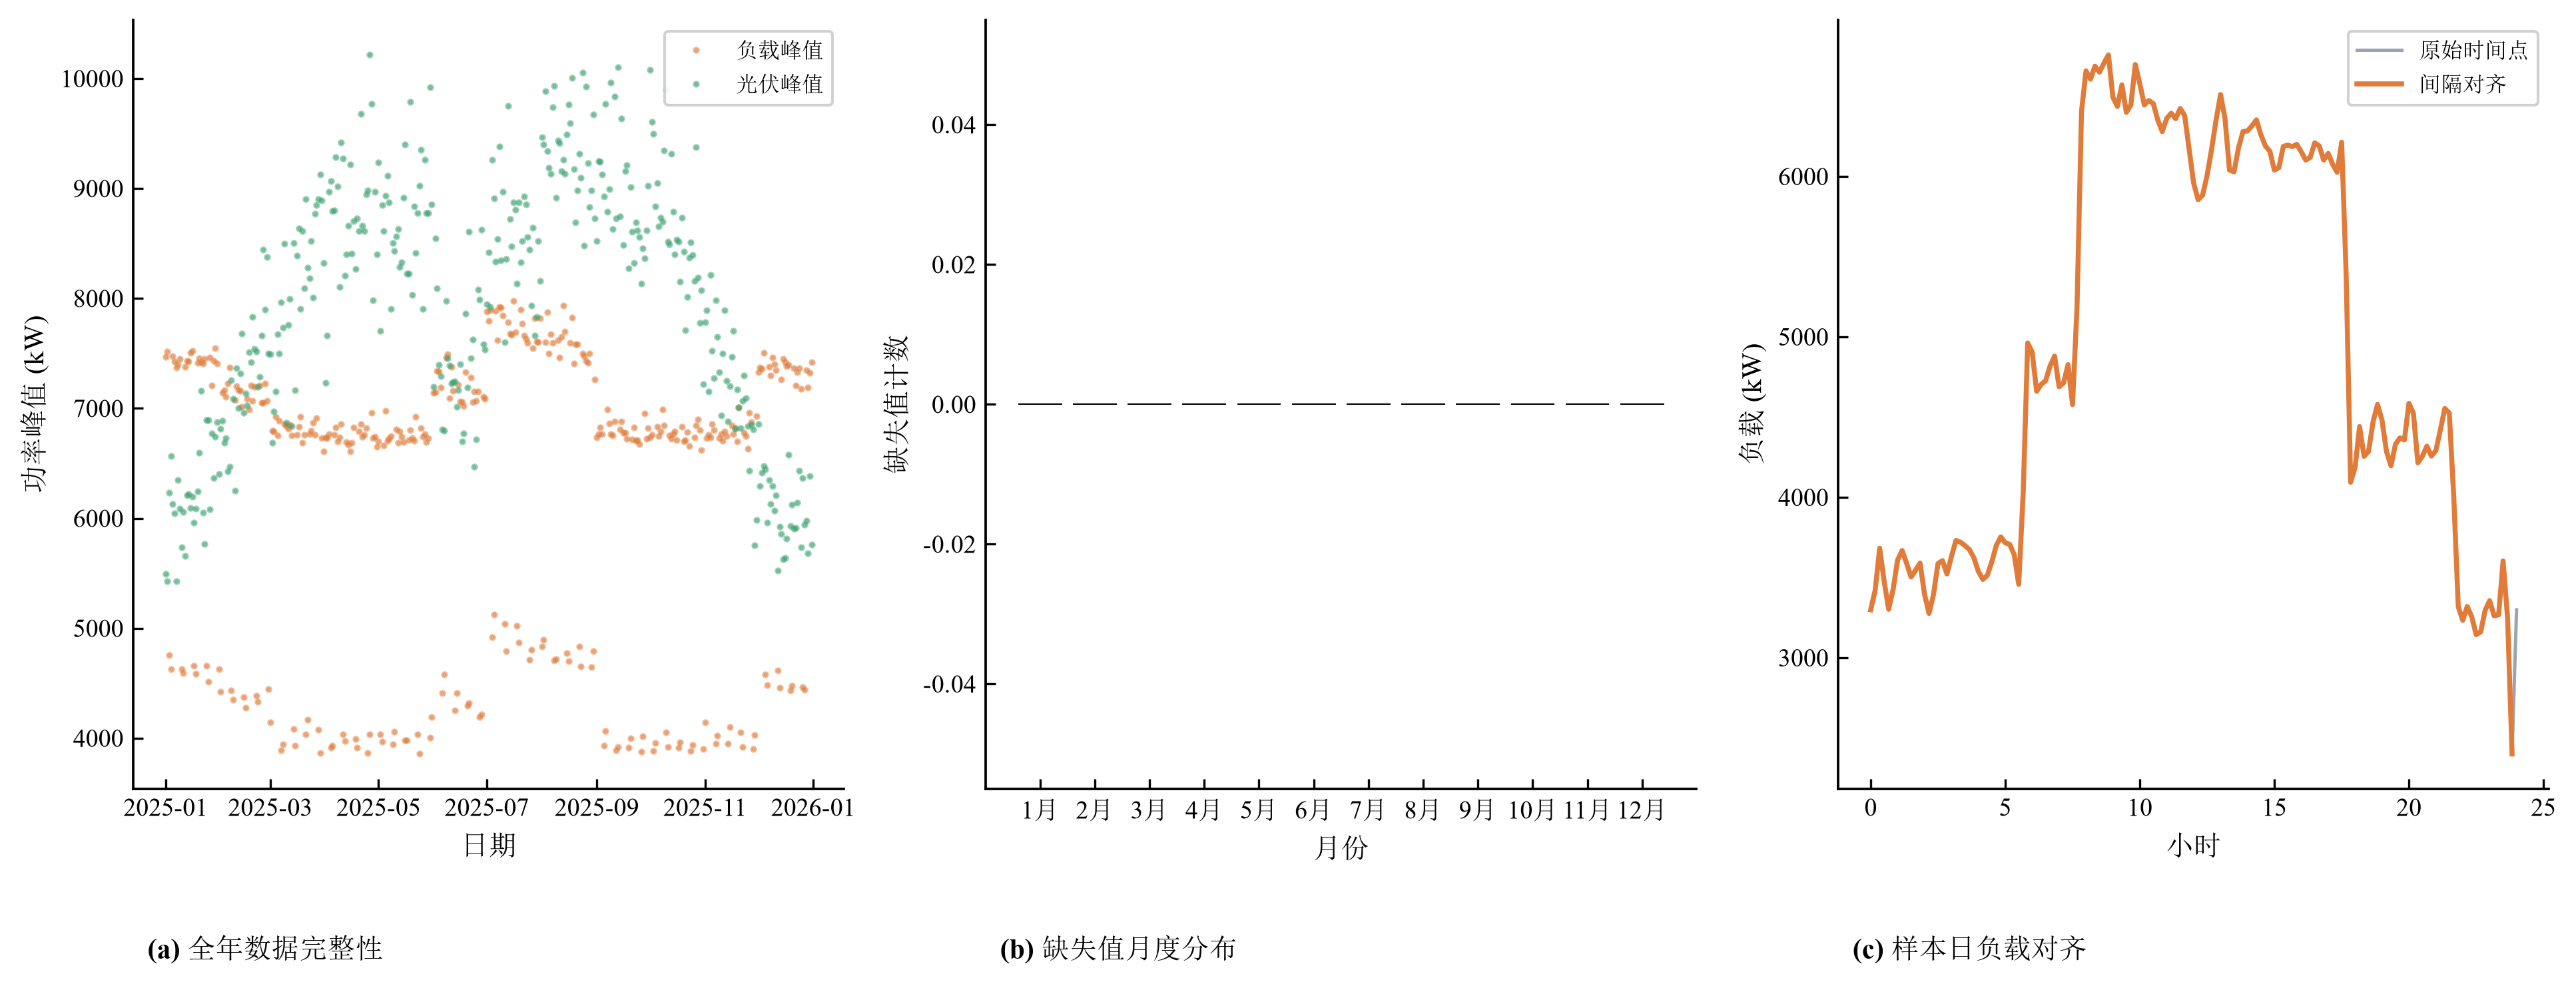
\includegraphics[width=0.72\textwidth]{求解/问题二/图片/图2-1_预处理前后对比.png}
    \caption{问题二全年数据预处理与完整性检查}
    \label{fig:preprocess2}
\end{figure}

由图\ref{fig:preprocess2}可知，全年负载与光伏峰值逐日变化，负载呈现明显的季节波动而光伏呈现冬低夏高的规律，且全年无缺失数据，样本日负载曲线在时间对齐后与原始时间点序列完全一致，数据质量良好。

需要说明的是，附件 2 的 365 天数据中，2025 年 1 月（1 月 1 日—1 月 31 日）作为\textbf{预热期}：模型以 1 月 1 日 0:00 储电量 6000 kWh 为初值逐日滚动，使储电量摆脱初始条件影响、进入稳定日循环（2 月 1 日 0:00 储电量已收敛至 1200 kWh 下限）；按照附件 5 的要求，结果文件与后文所有费用汇总均只统计 2025 年 2 月 1 日至 12 月 31 日共 334 天。

\textbf{2.算法选择}

在完成数据预处理后，本问需在全年尺度上求解 365 个逐日优化问题。与问题一相同，每个子问题均为线性规划，可直接沿用线性规划算法；区别在于需要设计日间储电量的传递机制。可从建模复杂度与全局最优性两个维度比较独立逐日求解与全年统一求解两种策略，如表\ref{tab:algo2}所示。

\begin{longtable}{>{\centering\arraybackslash}p{0.22\textwidth}>{\centering\arraybackslash}p{0.24\textwidth}>{\centering\arraybackslash}p{0.22\textwidth}>{\centering\arraybackslash}p{0.20\textwidth}}
  \caption{问题二求解策略对比}
  \label{tab:algo2} \\
  \toprule
  策略 & 建模复杂度 & 计算规模 & 最优性 \\
  \midrule
  \endfirsthead
  \caption{问题二求解策略对比（续）} \\
  \toprule
  策略 & 建模复杂度 & 计算规模 & 最优性 \\
  \midrule
  \endhead
  \bottomrule
  \endfoot
  全年统一求解 & 高 & 大规模 & 严格全局最优 \\
  逐日滚动求解 & 低 & 小规模 & 近似最优 \\
\end{longtable}

如\ref{tab:algo2}所示，全年统一求解虽在数学上严格，但变量规模达数十万，求解开销大；由于本问每日电价完全相同，日间不存在跨日套利空间，逐日滚动求解在储电量仅受上下限约束、无日末固定值的条件下，与全年统一求解的结果高度一致，且计算量小、易于解释。综合以上分析，本问选择逐日滚动线性规划策略进行求解。


% ════════════════════════════════════════════
% 模型建立（5.2.3.模型建立.tex，三级子块）
% ════════════════════════════════════════════
\subsubsection{模型建立}

针对问题二，本节在问题一线性规划模型基础上，将单日优化扩展为全年逐日滚动优化，并引入紧急购电费用。具体过程如下。

\textbf{步骤1：逐日优化模型}

对第 $d$ 天，决策变量仍为购电功率 $g_{d,k}$、充电功率 $c_{d,k}$、放电功率 $d_{d,k}$ 与储电量 $E_{d,k}$。该日优化目标为：
\begin{equation}
    \min \; Z_d=\sum_{k=0}^{143} g_{d,k}\,p_k\,\Delta t
\end{equation}
其中，$p_k$ 为附件一给出的与日期无关的分时电价。功率平衡约束与储能状态递推约束分别为：
\begin{equation}
    g_{d,k}+S_{d,k}+d_{d,k}-c_{d,k}\geq L_{d,k}
\end{equation}
\begin{equation}
    E_{d,k+1}=E_{d,k}+\eta\,c_{d,k}\,\Delta t-\frac{1}{\eta}\,d_{d,k}\,\Delta t
\end{equation}
容量与功率约束同问题一，即 $E_{\min}\leq E_{d,k}\leq E_{\max}$，$0\leq c_{d,k},d_{d,k}\leq P_{\max}$，$g_{d,k}\geq 0$。

\textbf{步骤2：日间储电量传递}

与问题一不同，问题二不再要求储电量在 0:00 与 24:00 相等，而是要求储电量在全年范围内连续传递。设第 $d$ 天的初值与末值分别为 $E_{d,0}$ 与 $E_{d,144}$，则相邻日的衔接关系为：
\begin{equation}
    E_{d+1,0}=E_{d,144},\quad d=0,1,\dots,363
\end{equation}
首日初值由附录一给定：
\begin{equation}
    E_{0,0}=6000
\end{equation}
由于每日电价相同，充放电存在约 $19\%$ 的往返损耗，最优解自然将每日末储电量放至下限附近，实现日内低充高放的套利最大化利用\cite{sioshansi2010}。

\textbf{步骤3：紧急购电费用}

问题二要求微网提供的电能不得低于小区负载，若低于负载则须以交易时刻电价 5 倍的价格向外网紧急购电。设第 $d$ 天第 $k$ 个间隔的实际供电缺口为 $\delta_{d,k}$，则：
\begin{equation}
    \delta_{d,k}=\max\{L_{d,k}-(g_{d,k}+S_{d,k}+d_{d,k}-c_{d,k}),\,0\}
\end{equation}
紧急购电费用为：
\begin{equation}
    Z^{\mathrm{em}}_d=\sum_{k=0}^{143} 5\,p_k\,\delta_{d,k}\,\Delta t
\end{equation}
由于本问在规划时已知附件二的真实负载与光伏，最优计划能够保证每个间隔供电不低于负载，因此 $\delta_{d,k}=0$，紧急购电费用为零，该机制主要作为问题三中预报偏差情形下的安全兜底。

\textbf{步骤4：全年总费用}

综上，问题二的全年总购电费用为各日购电费用与紧急购电费用之和：
\begin{equation}
    \min \; Z=\sum_{d=0}^{364}Z_d+\sum_{d=0}^{364}Z^{\mathrm{em}}_d
\end{equation}
\begin{equation}
    \mathrm{s.t.}\quad g_{d,k}+S_{d,k}+d_{d,k}-c_{d,k}\geq L_{d,k}
\end{equation}
\begin{equation}
    E_{d,k+1}=E_{d,k}+\eta\,c_{d,k}\,\Delta t-\frac{1}{\eta}\,d_{d,k}\,\Delta t
\end{equation}
\begin{equation}
    E_{\min}\leq E_{d,k}\leq E_{\max},\quad 0\leq c_{d,k},d_{d,k}\leq P_{\max},\quad g_{d,k}\geq 0
\end{equation}
\begin{equation}
    E_{d+1,0}=E_{d,144},\quad E_{0,0}=6000
\end{equation}
该模型按天递推求解 365 次，每次求解一个含 577 个变量的线性规划，既保证了计算的高效性，又通过储电量的逐日传递实现了全年尺度的协调优化。

综上所述，本节完成了问题二模型的建立，将单日线性规划推广为全年逐日滚动优化，并建立了紧急购电费用的惩罚机制，接下来将基于此进行求解。


% ════════════════════════════════════════════
% 模型求解（5.2.4.模型求解.tex，三级子块）
% ════════════════════════════════════════════
\subsubsection{模型求解}

基于上述模型，本节利用附件一与附件二数据逐日求解线性规划，得到全年 365 天的购电与充放电策略。其中 2025 年 1 月作为\textbf{预热期}：模型以 1 月 1 日 0:00 储电量 6000 kWh 为初值逐日滚动，使储电量摆脱初始条件影响、进入稳定的日循环（2 月 1 日 0:00 储电量已收敛至 1200 kWh 下限）；按照附件 5 的要求，结果文件与费用汇总均只统计 2025 年 2 月 1 日至 12 月 31 日（334 天），该口径下购电费用合计为 12254765.72 元，日均约 36690.92 元；由于规划时已知真实负载与光伏，紧急购电量为零。按题目要求，以表1的格式给出表3中四个指定日期在指定时间段的购电量及全天购电量、购电费（表\ref{tab:结果2-1a}～表\ref{tab:结果2-1d}），以表2的格式给出储能设备在指定时间段的充放电量及0:00和24:00储电量（表\ref{tab:结果2-2a}～表\ref{tab:结果2-2d}），并以表3的格式给出紧急购电结果（表\ref{tab:结果2-3}）；由于规划时已知真实负载与光伏，四个指定日期的紧急购电量均为零。

\begin{longtable}{>{\centering\arraybackslash}p{0.15\textwidth}>{\centering\arraybackslash}p{0.13\textwidth}>{\centering\arraybackslash}p{0.15\textwidth}>{\centering\arraybackslash}p{0.13\textwidth}>{\centering\arraybackslash}p{0.15\textwidth}>{\centering\arraybackslash}p{0.13\textwidth}}
  \caption{2025.3.20 微网在指定时间段的购电量及全天的购电量和购电费}
  \label{tab:结果2-1a} \\
  \toprule
  时间段 & 购电量 & 时间段 & 购电量 & 时间段 & 购电量 \\
  \midrule
  \endfirsthead
  \caption{2025.3.20 微网在指定时间段的购电量及全天的购电量和购电费（续）} \\
  \toprule
  时间段 & 购电量 & 时间段 & 购电量 & 时间段 & 购电量 \\
  \midrule
  \endhead
  \bottomrule
  \endfoot
  10:00--10:10 & 0.00 & 12:00--12:10 & 479.31 & 14:00--14:10 & 0.00 \\
  16:00--16:10 & 562.26 & 18:00--18:10 & 698.00 & 20:00--20:10 & 0.00 \\
  全天购电量 & 66322.04 & 全天购电费 & 40020.38 &  &  \\
\end{longtable}

\begin{longtable}{>{\centering\arraybackslash}p{0.15\textwidth}>{\centering\arraybackslash}p{0.13\textwidth}>{\centering\arraybackslash}p{0.15\textwidth}>{\centering\arraybackslash}p{0.13\textwidth}>{\centering\arraybackslash}p{0.15\textwidth}>{\centering\arraybackslash}p{0.13\textwidth}}
  \caption{2025.6.21 微网在指定时间段的购电量及全天的购电量和购电费}
  \label{tab:结果2-1b} \\
  \toprule
  时间段 & 购电量 & 时间段 & 购电量 & 时间段 & 购电量 \\
  \midrule
  \endfirsthead
  \caption{2025.6.21 微网在指定时间段的购电量及全天的购电量和购电费（续）} \\
  \toprule
  时间段 & 购电量 & 时间段 & 购电量 & 时间段 & 购电量 \\
  \midrule
  \endhead
  \bottomrule
  \endfoot
  10:00--10:10 & 0.00 & 12:00--12:10 & 0.00 & 14:00--14:10 & 0.00 \\
  16:00--16:10 & 78.57 & 18:00--18:10 & 0.00 & 20:00--20:10 & 0.00 \\
  全天购电量 & 32057.47 & 全天购电费 & 17599.36 &  &  \\
\end{longtable}

\begin{longtable}{>{\centering\arraybackslash}p{0.15\textwidth}>{\centering\arraybackslash}p{0.13\textwidth}>{\centering\arraybackslash}p{0.15\textwidth}>{\centering\arraybackslash}p{0.13\textwidth}>{\centering\arraybackslash}p{0.15\textwidth}>{\centering\arraybackslash}p{0.13\textwidth}}
  \caption{2025.9.23 微网在指定时间段的购电量及全天的购电量和购电费}
  \label{tab:结果2-1c} \\
  \toprule
  时间段 & 购电量 & 时间段 & 购电量 & 时间段 & 购电量 \\
  \midrule
  \endfirsthead
  \caption{2025.9.23 微网在指定时间段的购电量及全天的购电量和购电费（续）} \\
  \toprule
  时间段 & 购电量 & 时间段 & 购电量 & 时间段 & 购电量 \\
  \midrule
  \endhead
  \bottomrule
  \endfoot
  10:00--10:10 & 0.00 & 12:00--12:10 & 354.19 & 14:00--14:10 & 0.00 \\
  16:00--16:10 & 589.43 & 18:00--18:10 & 764.33 & 20:00--20:10 & 0.00 \\
  全天购电量 & 66265.42 & 全天购电费 & 41395.50 &  &  \\
\end{longtable}

\begin{longtable}{>{\centering\arraybackslash}p{0.15\textwidth}>{\centering\arraybackslash}p{0.13\textwidth}>{\centering\arraybackslash}p{0.15\textwidth}>{\centering\arraybackslash}p{0.13\textwidth}>{\centering\arraybackslash}p{0.15\textwidth}>{\centering\arraybackslash}p{0.13\textwidth}}
  \caption{2025.12.21 微网在指定时间段的购电量及全天的购电量和购电费}
  \label{tab:结果2-1d} \\
  \toprule
  时间段 & 购电量 & 时间段 & 购电量 & 时间段 & 购电量 \\
  \midrule
  \endfirsthead
  \caption{2025.12.21 微网在指定时间段的购电量及全天的购电量和购电费（续）} \\
  \toprule
  时间段 & 购电量 & 时间段 & 购电量 & 时间段 & 购电量 \\
  \midrule
  \endhead
  \bottomrule
  \endfoot
  10:00--10:10 & 0.00 & 12:00--12:10 & 932.83 & 14:00--14:10 & 0.00 \\
  16:00--16:10 & 801.38 & 18:00--18:10 & 715.41 & 20:00--20:10 & 0.00 \\
  全天购电量 & 93770.21 & 全天购电费 & 59747.81 &  &  \\
\end{longtable}

\begin{longtable}{>{\centering\arraybackslash}p{0.15\textwidth}>{\centering\arraybackslash}p{0.13\textwidth}>{\centering\arraybackslash}p{0.13\textwidth}>{\centering\arraybackslash}p{0.15\textwidth}>{\centering\arraybackslash}p{0.13\textwidth}>{\centering\arraybackslash}p{0.13\textwidth}}
  \caption{2025.3.20 储能设备在指定时间段的充放电量及0:00和24:00的储电量}
  \label{tab:结果2-2a} \\
  \toprule
  时间段 & 充电量 & 放电量 & 时间段 & 充电量 & 放电量 \\
  \midrule
  \endfirsthead
  \caption{2025.3.20 储能设备在指定时间段的充放电量及0:00和24:00的储电量（续）} \\
  \toprule
  时间段 & 充电量 & 放电量 & 时间段 & 充电量 & 放电量 \\
  \midrule
  \endhead
  \bottomrule
  \endfoot
  0:00--4:00 & 979.35 & 0.00 & 4:00--8:00 & 833.33 & 1468.27 \\
  8:00--12:00 & 2925.38 & 0.00 & 12:00--16:00 & 7741.29 & 0.00 \\
  16:00--20:00 & 0.00 & 6252.90 & 20:00--24:00 & 0.00 & 2387.10 \\
  0:00储电量 & 1200.00 &  & 24:00储电量 & 1200.00 &  \\
\end{longtable}

\begin{longtable}{>{\centering\arraybackslash}p{0.15\textwidth}>{\centering\arraybackslash}p{0.13\textwidth}>{\centering\arraybackslash}p{0.13\textwidth}>{\centering\arraybackslash}p{0.15\textwidth}>{\centering\arraybackslash}p{0.13\textwidth}>{\centering\arraybackslash}p{0.13\textwidth}}
  \caption{2025.6.21 储能设备在指定时间段的充放电量及0:00和24:00的储电量}
  \label{tab:结果2-2b} \\
  \toprule
  时间段 & 充电量 & 放电量 & 时间段 & 充电量 & 放电量 \\
  \midrule
  \endfirsthead
  \caption{2025.6.21 储能设备在指定时间段的充放电量及0:00和24:00的储电量（续）} \\
  \toprule
  时间段 & 充电量 & 放电量 & 时间段 & 充电量 & 放电量 \\
  \midrule
  \endhead
  \bottomrule
  \endfoot
  0:00--4:00 & 9000.00 & 0.00 & 4:00--8:00 & 1666.67 & 6927.39 \\
  8:00--12:00 & 5154.73 & 1712.61 & 12:00--16:00 & 5604.34 & 74.85 \\
  16:00--20:00 & 0.00 & 5576.93 & 20:00--24:00 & 0.00 & 3063.07 \\
  0:00储电量 & 1200.00 &  & 24:00储电量 & 1200.00 &  \\
\end{longtable}

\begin{longtable}{>{\centering\arraybackslash}p{0.15\textwidth}>{\centering\arraybackslash}p{0.13\textwidth}>{\centering\arraybackslash}p{0.13\textwidth}>{\centering\arraybackslash}p{0.15\textwidth}>{\centering\arraybackslash}p{0.13\textwidth}>{\centering\arraybackslash}p{0.13\textwidth}}
  \caption{2025.9.23 储能设备在指定时间段的充放电量及0:00和24:00的储电量}
  \label{tab:结果2-2c} \\
  \toprule
  时间段 & 充电量 & 放电量 & 时间段 & 充电量 & 放电量 \\
  \midrule
  \endfirsthead
  \caption{2025.9.23 储能设备在指定时间段的充放电量及0:00和24:00的储电量（续）} \\
  \toprule
  时间段 & 充电量 & 放电量 & 时间段 & 充电量 & 放电量 \\
  \midrule
  \endhead
  \bottomrule
  \endfoot
  0:00--4:00 & 9000.00 & 0.00 & 4:00--8:00 & 1666.67 & 6577.11 \\
  8:00--12:00 & 5512.02 & 2062.89 & 12:00--16:00 & 5236.78 & 66.53 \\
  16:00--20:00 & 0.00 & 6336.19 & 20:00--24:00 & 0.00 & 2303.81 \\
  0:00储电量 & 1200.00 &  & 24:00储电量 & 1200.00 &  \\
\end{longtable}

\begin{longtable}{>{\centering\arraybackslash}p{0.15\textwidth}>{\centering\arraybackslash}p{0.13\textwidth}>{\centering\arraybackslash}p{0.13\textwidth}>{\centering\arraybackslash}p{0.15\textwidth}>{\centering\arraybackslash}p{0.13\textwidth}>{\centering\arraybackslash}p{0.13\textwidth}}
  \caption{2025.12.21 储能设备在指定时间段的充放电量及0:00和24:00的储电量}
  \label{tab:结果2-2d} \\
  \toprule
  时间段 & 充电量 & 放电量 & 时间段 & 充电量 & 放电量 \\
  \midrule
  \endfirsthead
  \caption{2025.12.21 储能设备在指定时间段的充放电量及0:00和24:00的储电量（续）} \\
  \toprule
  时间段 & 充电量 & 放电量 & 时间段 & 充电量 & 放电量 \\
  \midrule
  \endhead
  \bottomrule
  \endfoot
  0:00--4:00 & 9000.00 & 0.00 & 4:00--8:00 & 2500.00 & 1508.33 \\
  8:00--12:00 & 5833.33 & 7806.67 & 12:00--16:00 & 7717.70 & 2336.33 \\
  16:00--20:00 & 0.00 & 5737.84 & 20:00--24:00 & 0.00 & 2902.16 \\
  0:00储电量 & 1200.00 &  & 24:00储电量 & 1200.00 &  \\
\end{longtable}

\begin{longtable}{>{\centering\arraybackslash}p{0.11\textwidth}>{\centering\arraybackslash}p{0.08\textwidth}>{\centering\arraybackslash}p{0.11\textwidth}>{\centering\arraybackslash}p{0.08\textwidth}>{\centering\arraybackslash}p{0.11\textwidth}>{\centering\arraybackslash}p{0.08\textwidth}>{\centering\arraybackslash}p{0.11\textwidth}>{\centering\arraybackslash}p{0.08\textwidth}}
  \caption{微网在指定日期的紧急购电量}
  \label{tab:结果2-3} \\
  \toprule
  \multicolumn{2}{c}{2025.3.20} & \multicolumn{2}{c}{2025.6.21} & \multicolumn{2}{c}{2025.9.23} & \multicolumn{2}{c}{2025.12.21} \\
  \cmidrule(lr){1-2} \cmidrule(lr){3-4} \cmidrule(lr){5-6} \cmidrule(lr){7-8}
  时间段 & 购电量 & 时间段 & 购电量 & 时间段 & 购电量 & 时间段 & 购电量 \\
  \midrule
  \endfirsthead
  \caption{微网在指定日期的紧急购电量（续）} \\
  \toprule
  \multicolumn{2}{c}{2025.3.20} & \multicolumn{2}{c}{2025.6.21} & \multicolumn{2}{c}{2025.9.23} & \multicolumn{2}{c}{2025.12.21} \\
  \cmidrule(lr){1-2} \cmidrule(lr){3-4} \cmidrule(lr){5-6} \cmidrule(lr){7-8}
  时间段 & 购电量 & 时间段 & 购电量 & 时间段 & 购电量 & 时间段 & 购电量 \\
  \midrule
  \endhead
  \bottomrule
  \endfoot
  --- & 0.00 & --- & 0.00 & --- & 0.00 & --- & 0.00 \\
\end{longtable}

2.1—12.31 逐日购电费用及其 7 日滑动平均如图\ref{fig:结果2-2}所示。可以看出，购电费呈现明显的季节性波动：冬季（12 月）因光伏出力低、负荷高，购电费最高；夏季（6 月）因光伏出力充沛，购电费最低，与光伏资源的季节规律一致。

\begin{figure}[H]
    \centering
    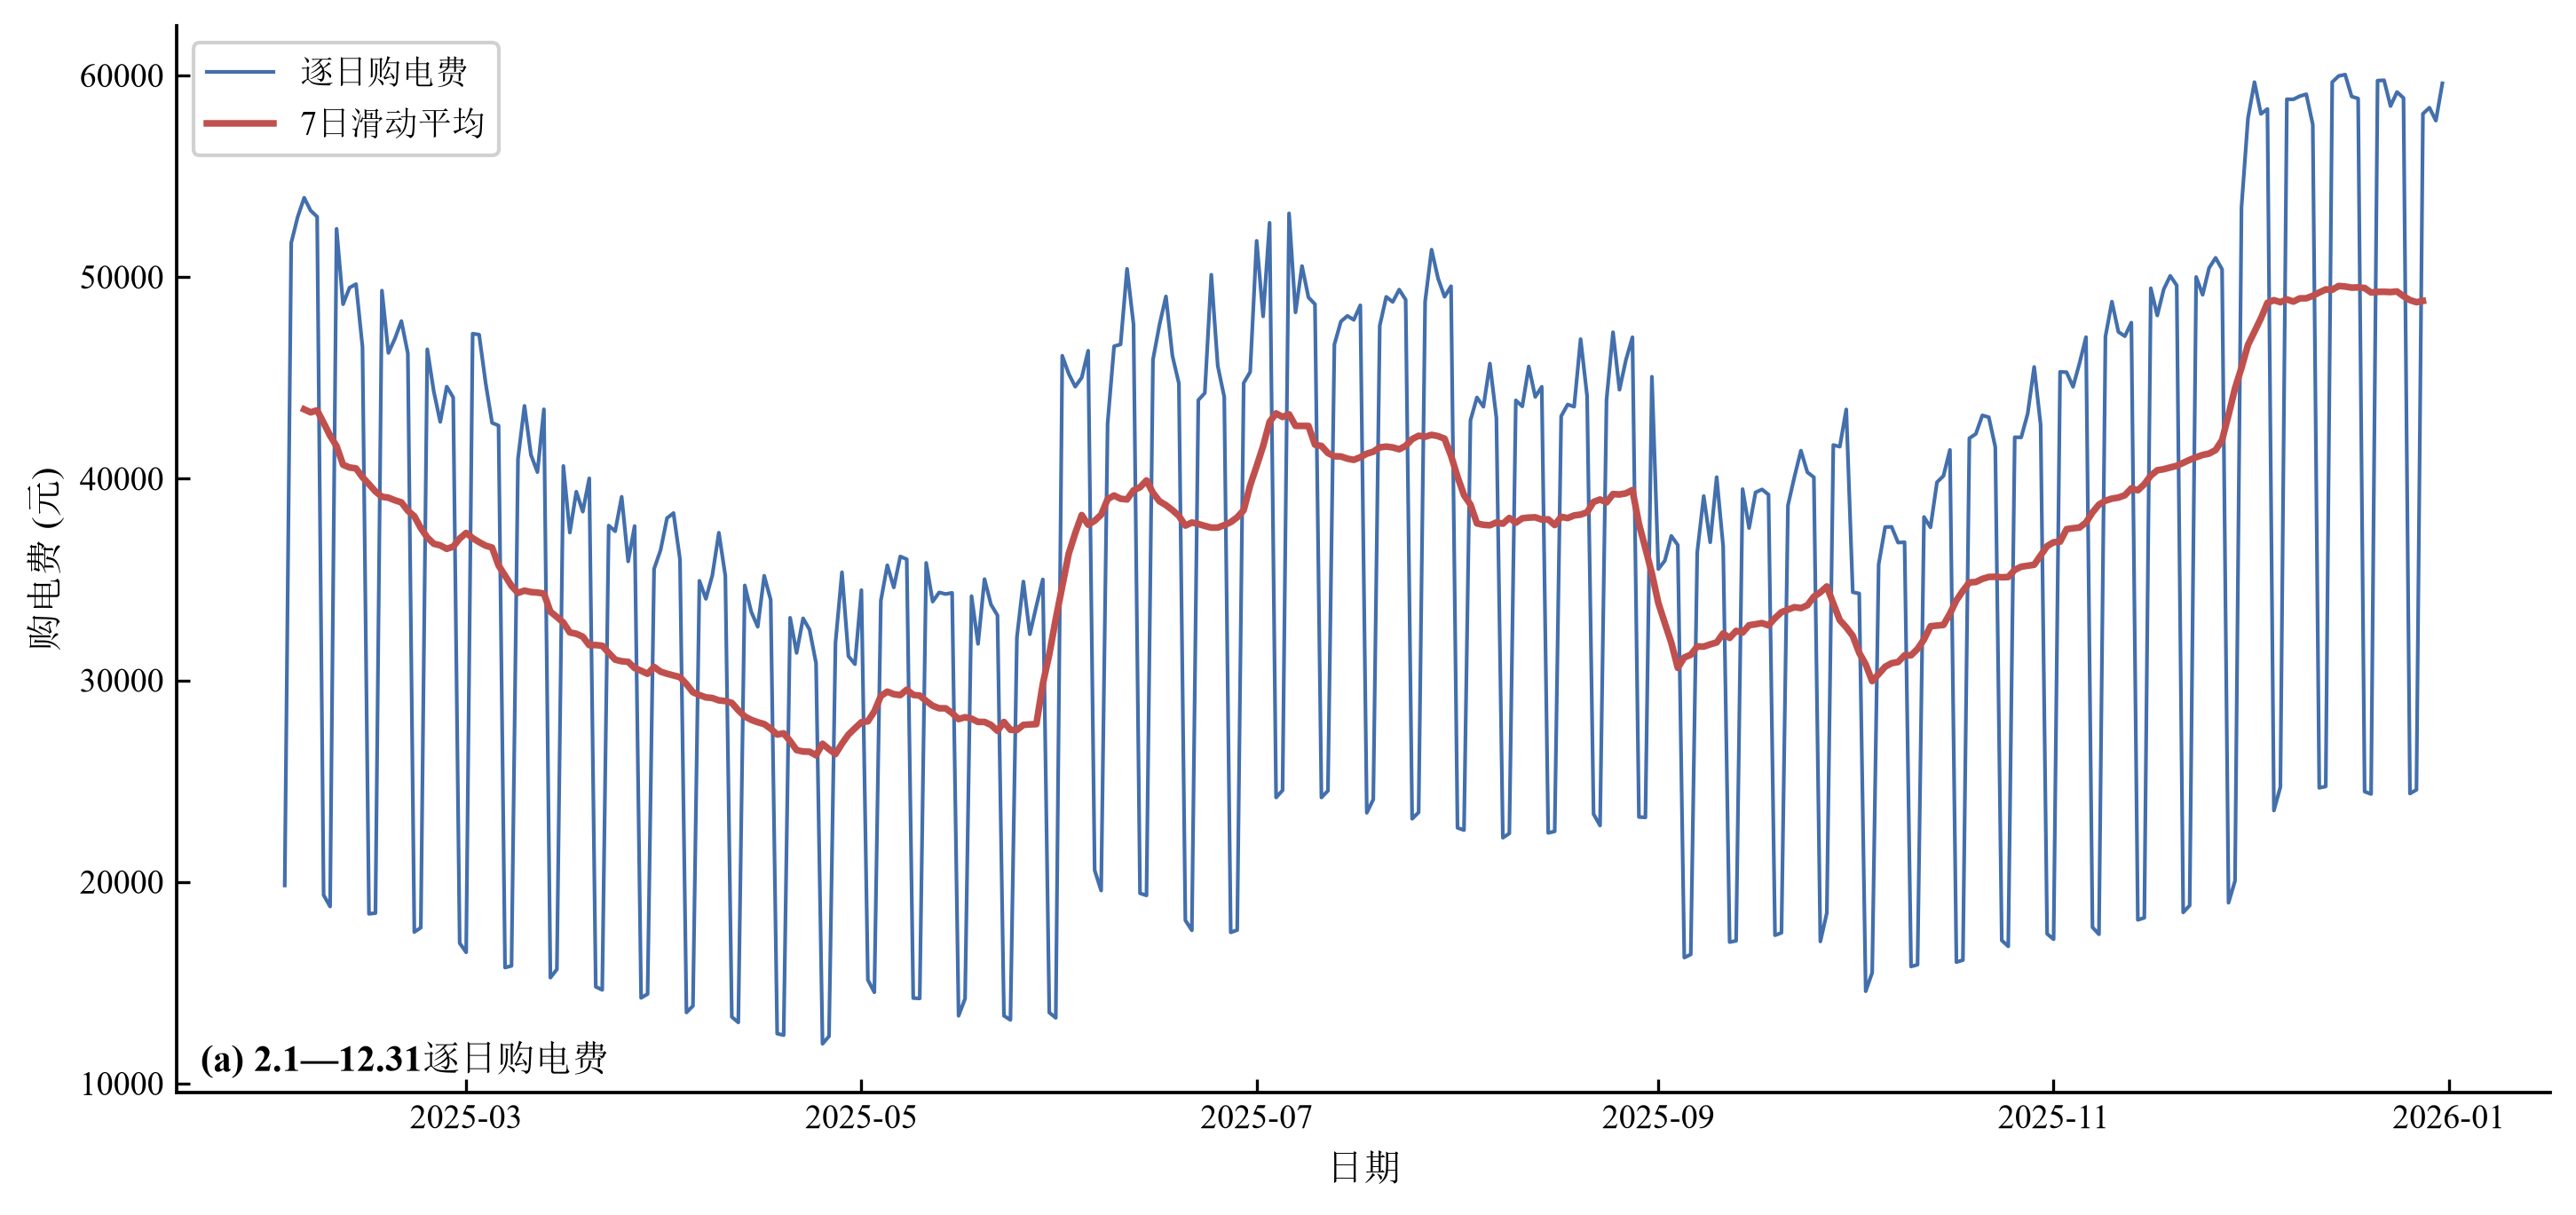
\includegraphics[width=0.70\textwidth]{求解/问题二/图片/图2-2_全年逐日购电费.png}
    \caption{2.1—12.31逐日购电费及7日滑动平均}
    \label{fig:结果2-2}
\end{figure}

四季典型日的购电功率曲线如图\ref{fig:结果2-3}所示。四个季节的购电功率均集中在夜间低电价时段，白天因光伏与储能放电的支撑，购电功率显著减小；冬季典型日购电功率整体最高，与表\ref{tab:结果2-1d}中冬季购电费最高相吻合。

\begin{figure}[H]
    \centering
    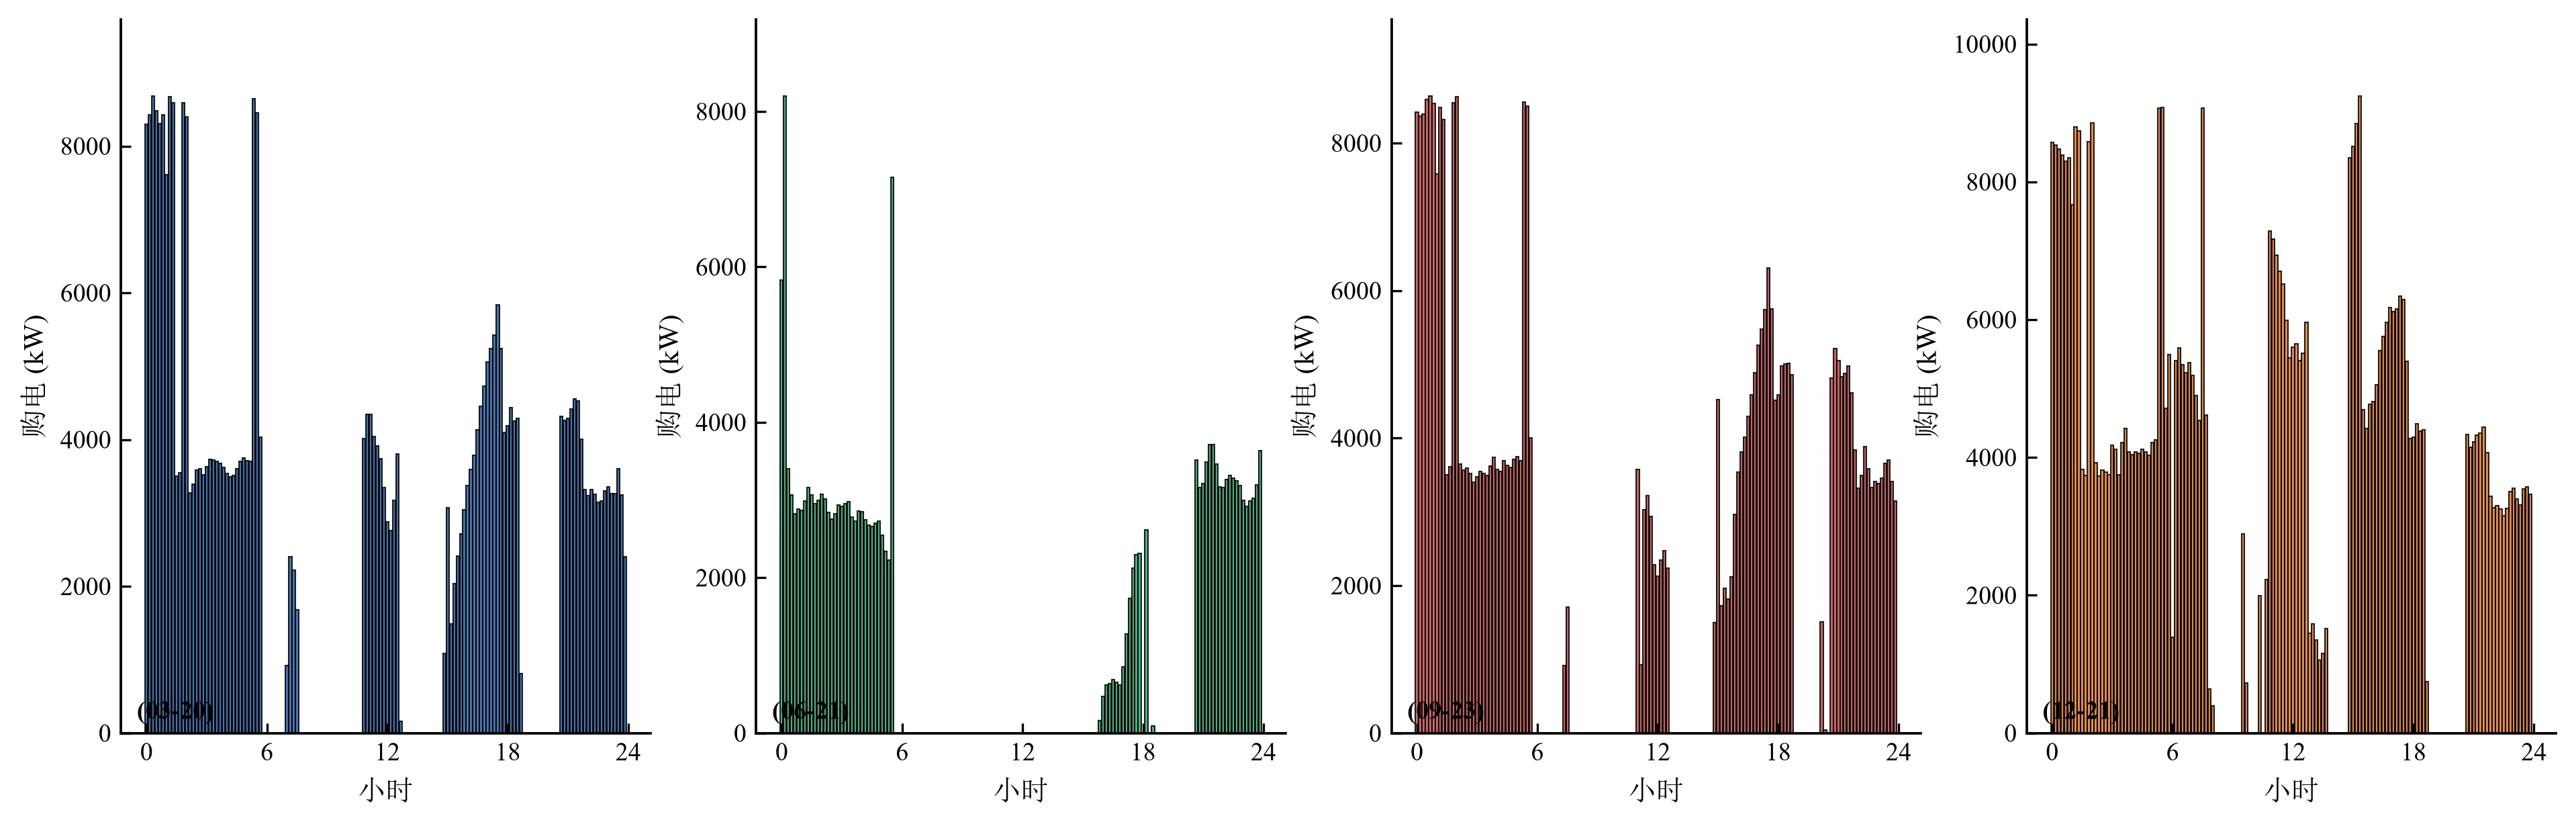
\includegraphics[width=0.75\textwidth]{求解/问题二/图片/图2-3_四季典型日购电策略.png}
    \caption{四季典型日的购电功率策略}
    \label{fig:结果2-3}
\end{figure}

四季典型日的储能荷电状态轨迹如图\ref{fig:结果2-4}所示。储能荷电状态每日在 1200 kWh 与 10800 kWh 之间完成一次充放循环，白天光伏盈余时充电、夜间与傍晚放电，且全天严格处于约束区间内，验证了滚动模型的可行性。

\begin{figure}[H]
    \centering
    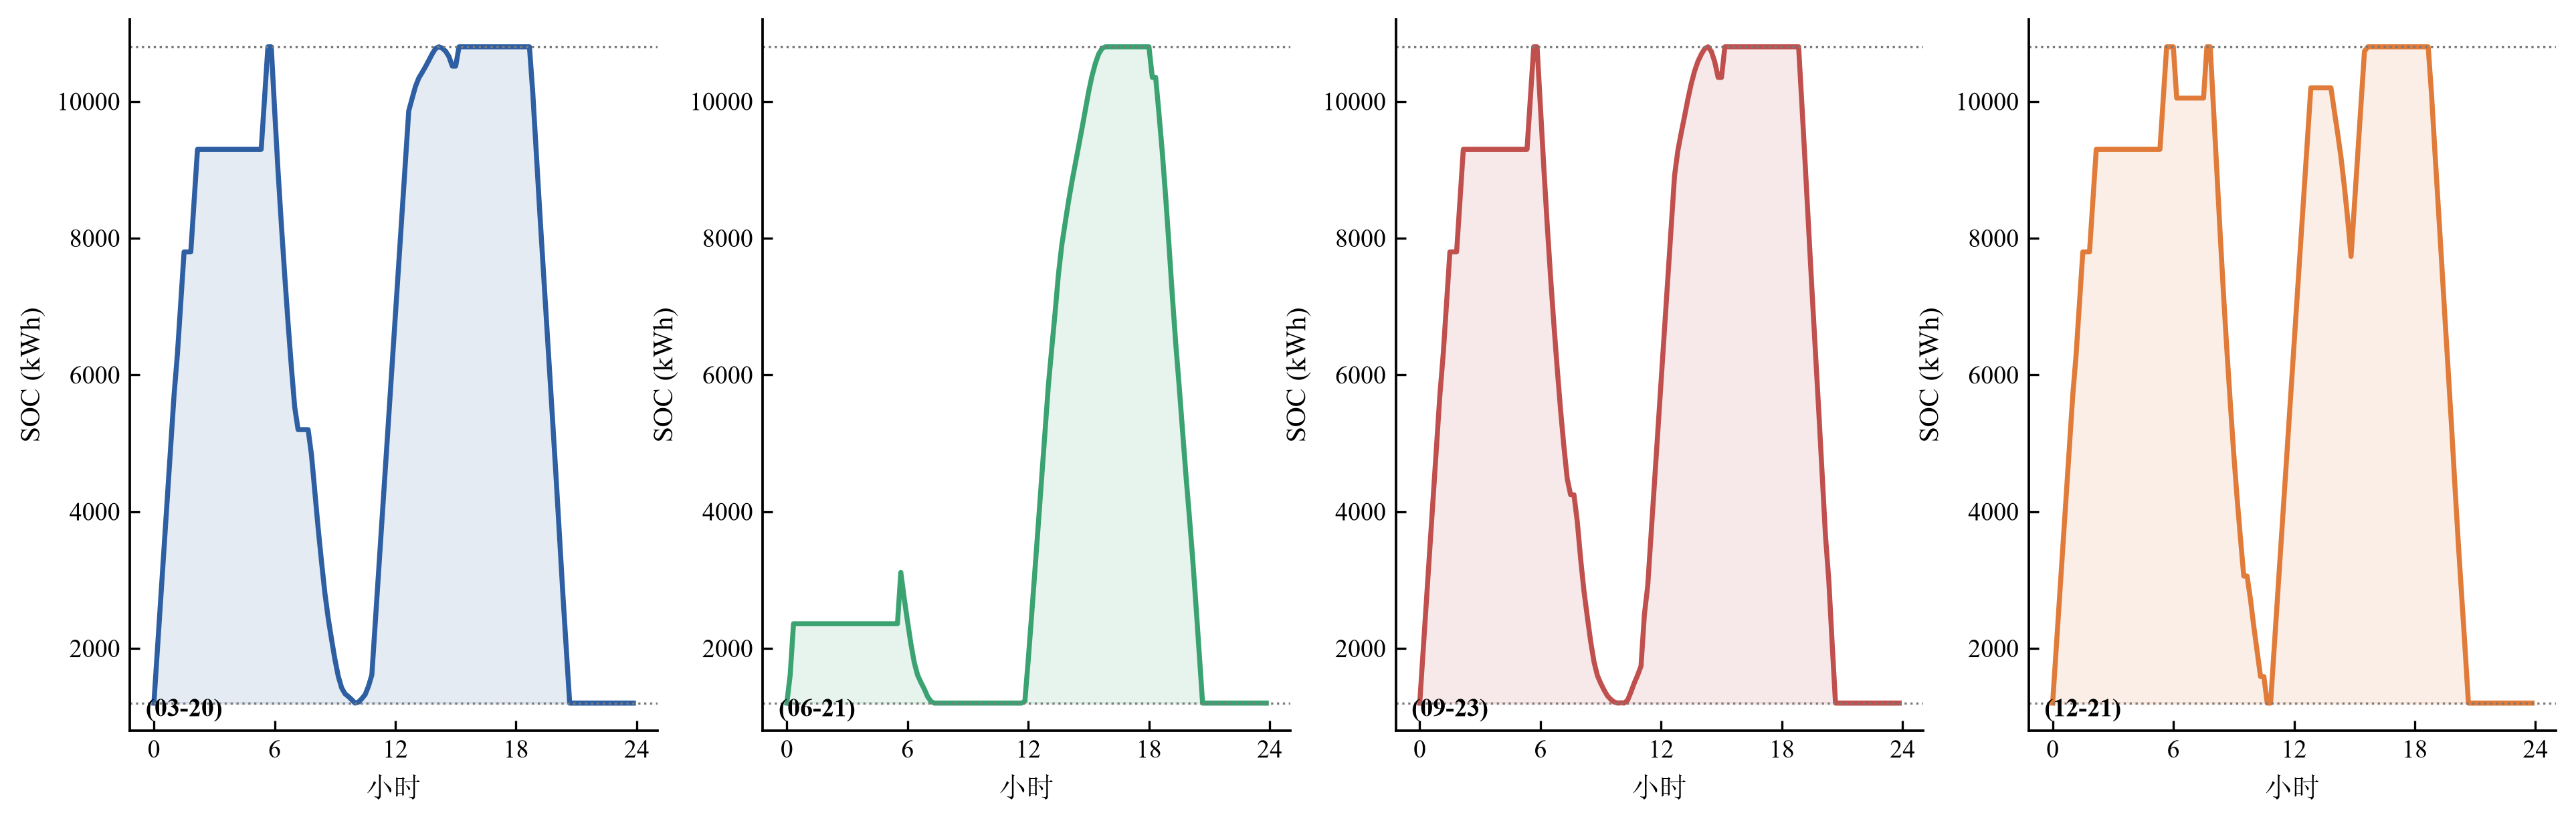
\includegraphics[width=0.75\textwidth]{求解/问题二/图片/图2-4_四季典型日SOC轨迹.png}
    \caption{四季典型日储能荷电状态轨迹}
    \label{fig:结果2-4}
\end{figure}

2—12 月储能每日 0:00 储电量的月度分布如图\ref{fig:结果2-5}所示。各月储电量中位数均处于 1200 kWh 附近，说明储能每日末放至下限的规律在全年保持稳定，符合低充高放套利的最优行为。

\begin{figure}[H]
    \centering
    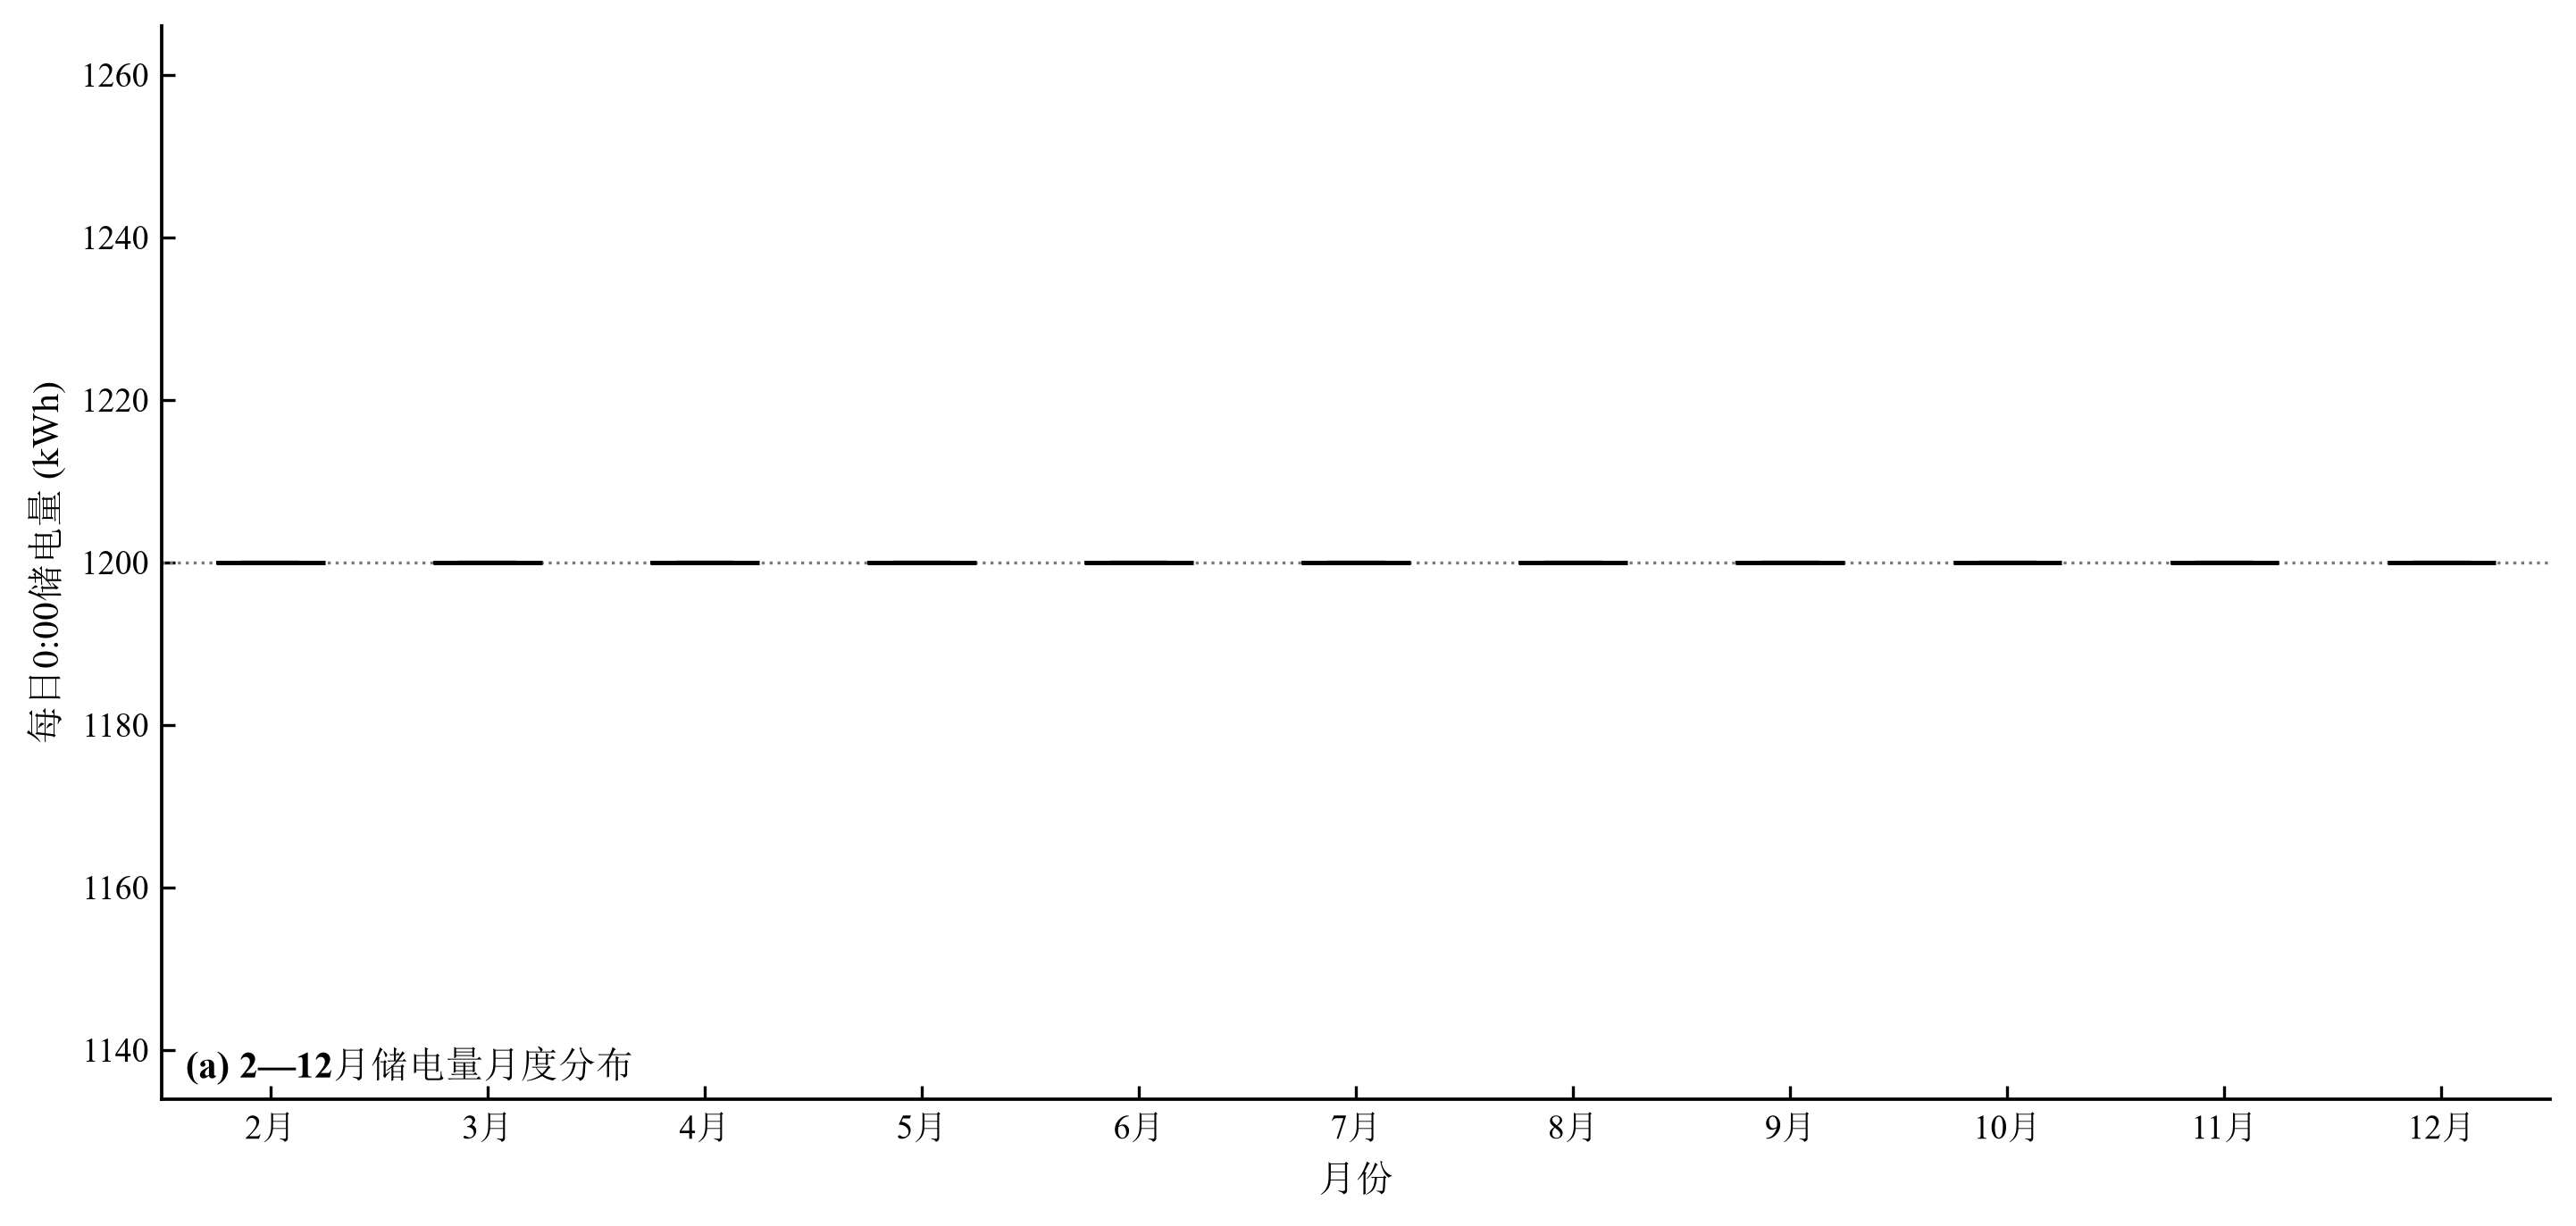
\includegraphics[width=0.70\textwidth]{求解/问题二/图片/图2-5_全年储能SOC月度分布.png}
    \caption{储能每日0:00储电量月度分布（2—12月）}
    \label{fig:结果2-5}
\end{figure}

购电功率与净负荷的关系（2.1—12.31）及月度购电费（2—12月）如图\ref{fig:结果2-6}所示。日均购电功率与日均净负荷呈显著正相关，负荷越大、光伏越小则购电越多；月度购电费在冬季达到峰值、夏季为谷值，进一步印证了模型的合理性。

\begin{figure}[H]
    \centering
    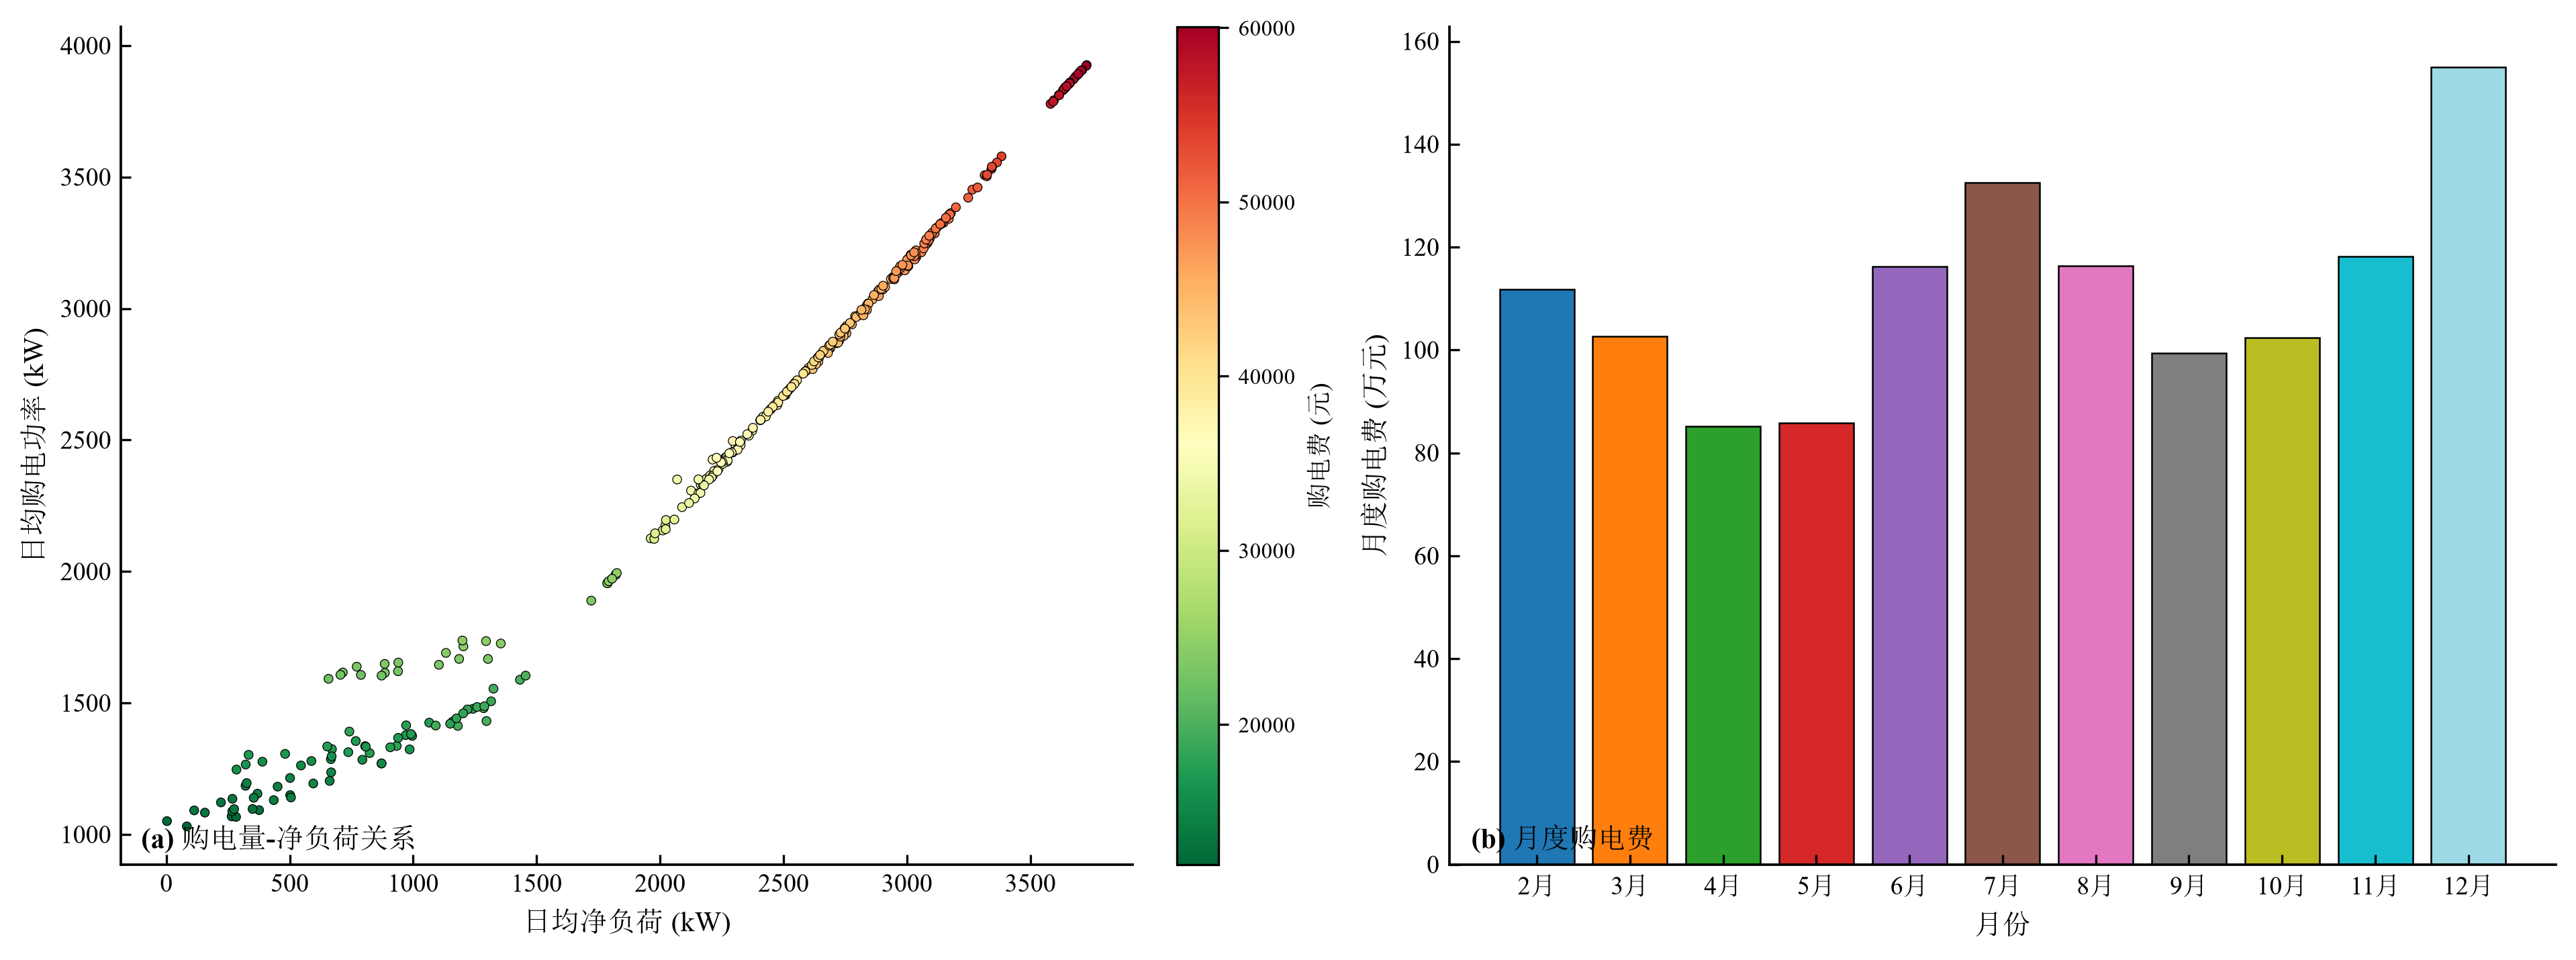
\includegraphics[width=0.72\textwidth]{求解/问题二/图片/图2-6_购电量与净负荷关系.png}
    \caption{购电功率与净负荷的关系及月度购电费}
    \label{fig:结果2-6}
\end{figure}

综合以上结果，问题二的逐日滚动线性规划模型在全年的负载与光伏变化下，通过储能的低充高放显著削减了购电费用，供电缺口恒为零、紧急购电量为零，模型与结果均合理可靠。



% ════════════════════════════════════════════
% 单个问题的建立求解（5.3.问题三.tex，二级标题包装）
% ════════════════════════════════════════════
\subsection{问题三的模型的建立和求解}


% ════════════════════════════════════════════
% 具体分析（5.3.1.具体分析.tex，三级子块）
% ════════════════════════════════════════════
\subsubsection{具体分析}

针对问题三，本问属于滚动预测下的随机调度与调整优化类问题，采用滚动时域线性规划方法，在 0:00、6:00、12:00 与 18:00 四个预报时刻依次制定计划购电与调整购电策略，并引入违约惩罚与超额电价机制。

本文先将附件三中四时刻发布的小时光伏预报插值到 10 分钟分辨率，形成可逐间隔使用的功率序列；在 0:00 依据最新预报制定全天计划购电策略；在 6:00、12:00、18:00 依据不断更新的预报对剩余时段进行滚动调整，其中计划购电量高于调整购电量的部分按交易电价 50\% 计违约费用，调整购电量高于计划购电量的部分按交易电价 1.5 倍计价；最后以实际供电缺口核算 5 倍电价的紧急购电费用，得到全年总购电费用并分析引入其他预报时刻调整的收益（1 月为预热期，费用汇总仅统计 2 月 1 日—12 月 31 日）。具体分析流程如图\ref{fig:analysis3_flow}所示。

\begin{figure}[H]
    \begin{center}
        \begin{tikzpicture}[x=1cm, y=0.75cm,
            flowhead/.style={rectangle, rounded corners=3pt, draw=orange!80!black, fill=orange!55!black, text=white, font=\bfseries, minimum width=7.2cm, minimum height=1.1cm, align=center, inner sep=2pt, line width=0.7pt},
            flowbox/.style={rectangle, rounded corners=2.5pt, draw=orange!70!black, fill=orange!14, minimum width=7.2cm, minimum height=1.0cm, align=center, inner sep=2pt, line width=0.6pt},
            flowend/.style={rectangle, rounded corners=2.5pt, draw=orange!85!black, fill=orange!45!black, text=white, font=\bfseries, minimum width=7.2cm, minimum height=1.0cm, align=center, inner sep=2pt, line width=0.7pt},
            flowarrow/.style={thick, -{Stealth}, orange!60!black}
        ]
            \node[flowhead] at (0, 0) (h) {问题三：滚动预报与调整优化};
            \node[flowbox] at (0, -1.8) (s1) {\textbf{光伏预报插值}\\\footnotesize 四时刻小时预报插值到 10 分钟};
            \node[flowbox] at (0, -3.6) (s2) {\textbf{0:00 制定计划}\\\footnotesize 依最新预报制定全天购电计划};
            \node[flowbox] at (0, -5.4) (s3) {\textbf{6:00 滚动调整}\\\footnotesize 更新预报并调整剩余时段购电};
            \node[flowbox] at (0, -7.2) (s4) {\textbf{12:00 滚动调整}\\\footnotesize 更新预报并调整剩余时段购电};
            \node[flowbox] at (0, -9.0) (s5) {\textbf{18:00 滚动调整}\\\footnotesize 更新预报并调整剩余时段购电};
            \node[flowbox] at (0, -10.8) (s6) {\textbf{分段惩罚计价}\\\footnotesize 不足按 50\% · 超额按 1.5 倍};
            \node[flowbox] at (0, -12.6) (s7) {\textbf{紧急购电核算}\\\footnotesize 实际供电缺口按 5 倍电价计费};
            \node[flowend] at (0, -14.4) (s8) {2.1—12.31费用汇总\\\footnotesize 输出总购电费用与调整收益};
            \draw[flowarrow] (h) -- (s1);
            \draw[flowarrow] (s1) -- (s2);
            \draw[flowarrow] (s2) -- (s3);
            \draw[flowarrow] (s3) -- (s4);
            \draw[flowarrow] (s4) -- (s5);
            \draw[flowarrow] (s5) -- (s6);
            \draw[flowarrow] (s6) -- (s7);
            \draw[flowarrow] (s7) -- (s8);
        \end{tikzpicture}
        \caption{问题三分析流程图}
        \label{fig:analysis3_flow}
    \end{center}
\end{figure}


% ════════════════════════════════════════════
% 模型准备（5.3.2.模型准备.tex，三级子块）
% ════════════════════════════════════════════
\subsubsection{模型准备}

\textbf{1.数据预处理}

附件三给出了 2025 年全年每天 0:00、6:00、12:00、18:00 四个时刻发布的未来 24 小时整点光伏发电功率预报，而实际负载与光伏功率的时间分辨率均为 10 分钟，因此需要将小时分辨率的光伏预报插值到 10 分钟间隔上。设某预报时刻 $\tau$ 发布的第 $n$ 小时预报功率为 $f_n$，其对应时刻为 $\tau+n$（小时），则预报序列在小时尺度上给出了一组离散点 $(\tau,f_0),(\tau+1,f_1),\dots,(\tau+24,f_{23})$。对第 $k$ 个间隔末端时刻 $t_k=(k+1)/6$（小时）进行线性插值，得到：
\begin{equation}
    S^{\tau}_k=\mathrm{interp}\big(t_k;\,\{\tau+j\}_{j=0}^{24},\,\{f_{j-1}\}_{j=1}^{24}\big)
\end{equation}
其中，$f_0$ 取 $f_1$ 近似当前整点功率，$S^{\tau}_k$ 为预报时刻 $\tau$ 发布的第 $k$ 个间隔的光伏预报功率。各预报时刻的实际预报与真实光伏对比如图\ref{fig:preprocess3}所示。

\begin{figure}[H]
    \centering
    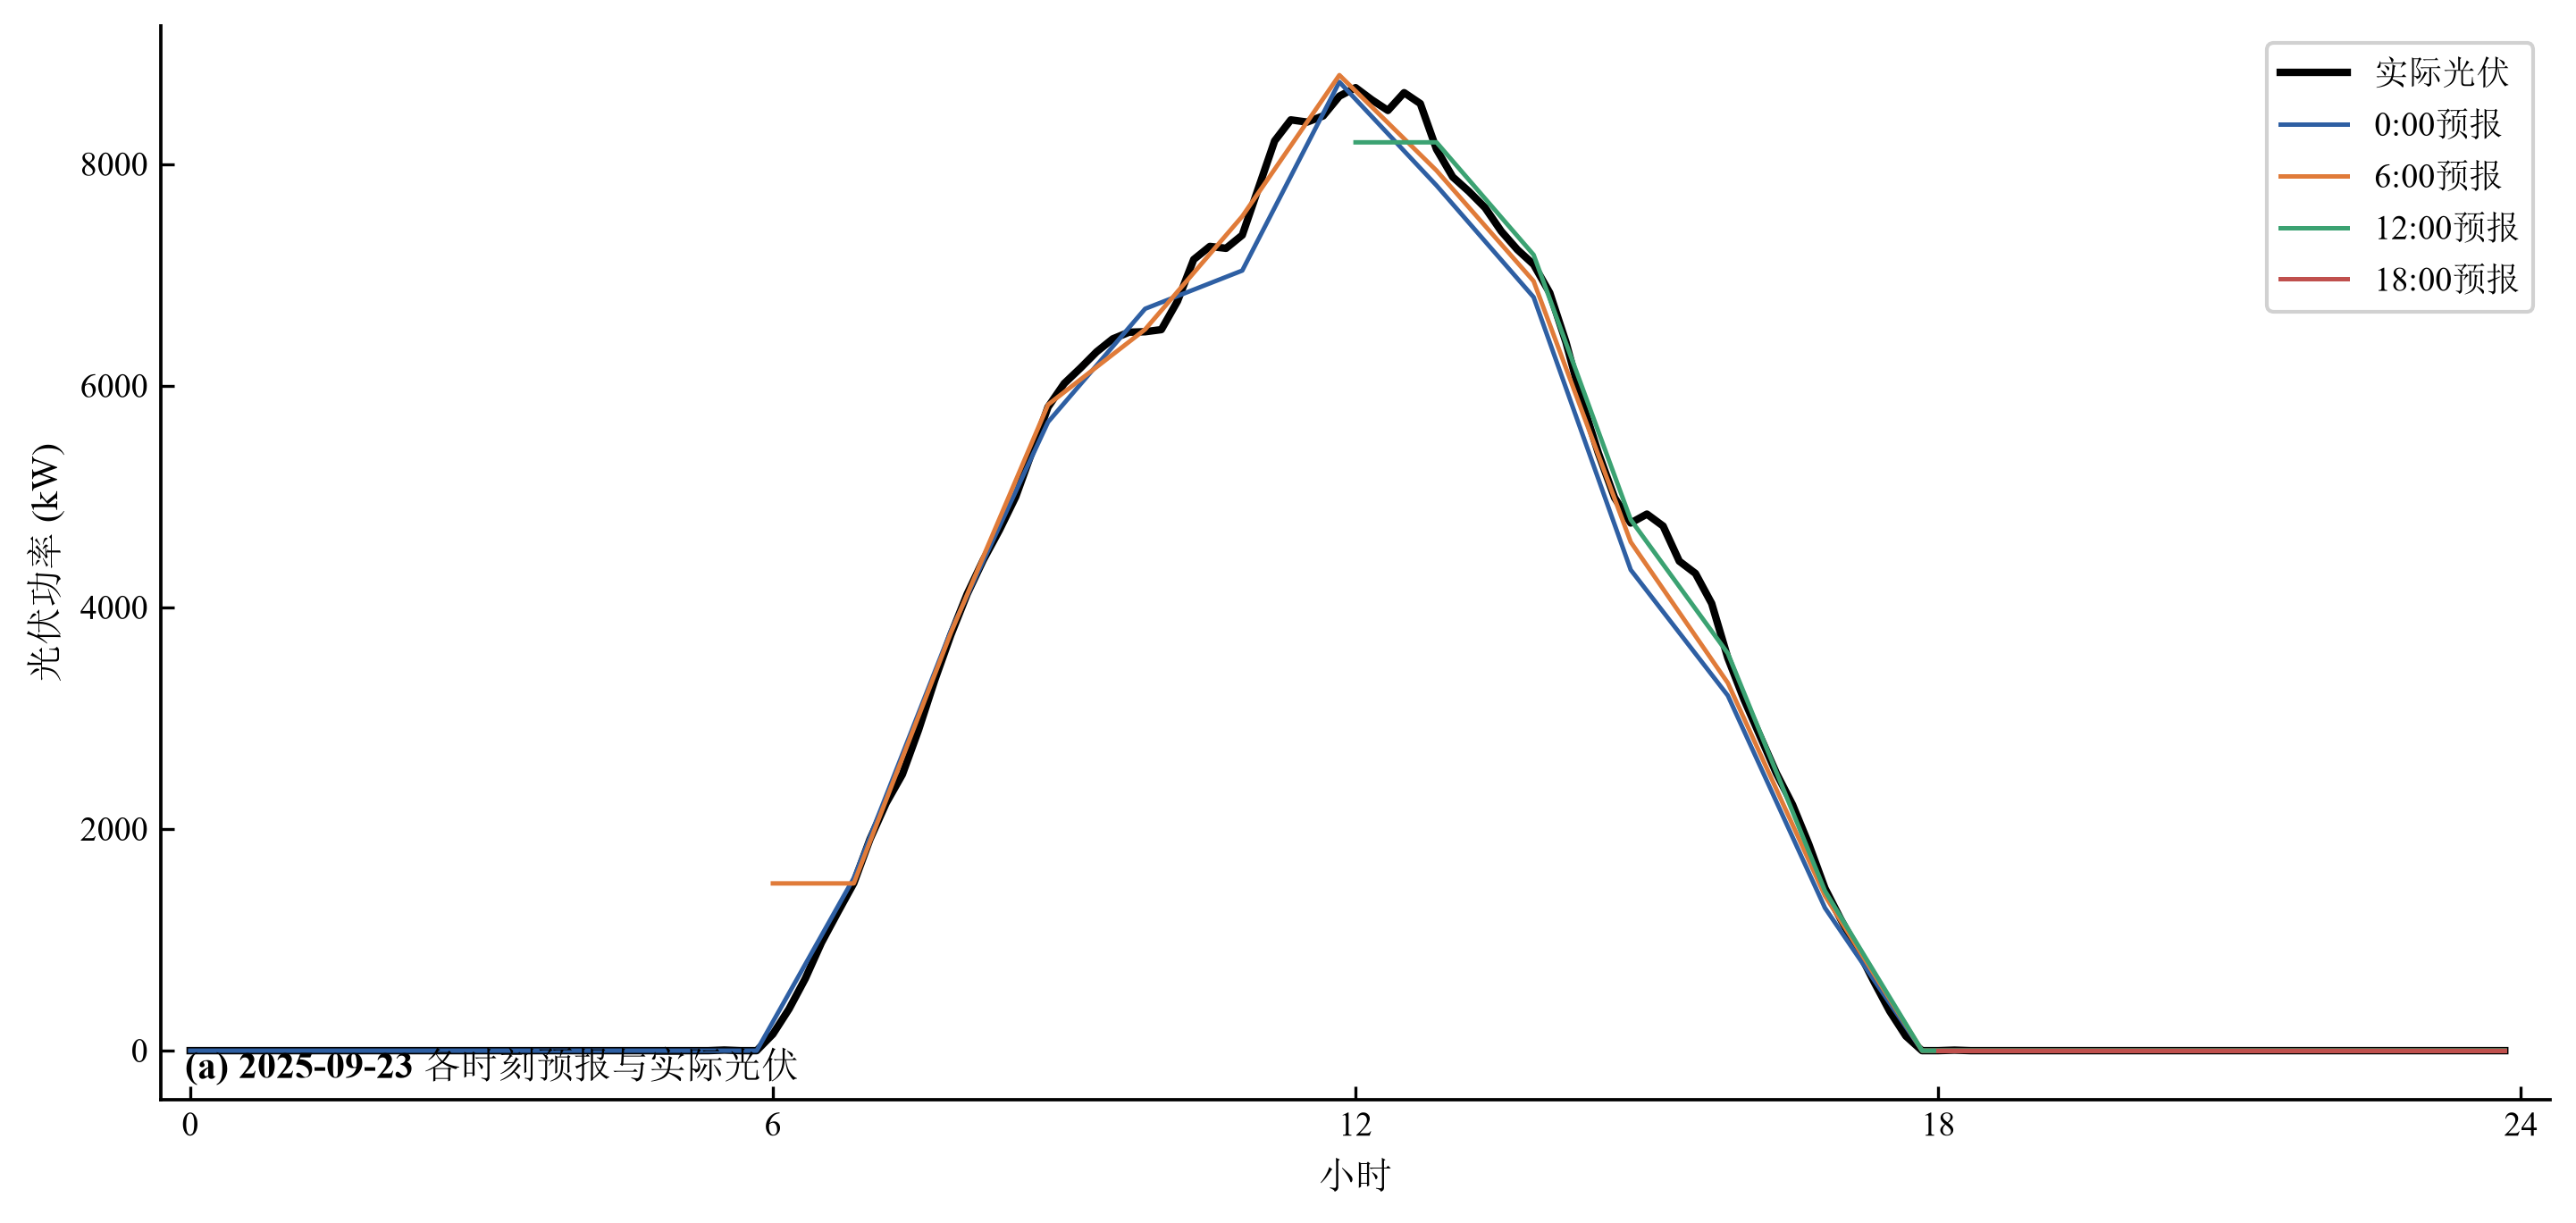
\includegraphics[width=0.70\textwidth]{求解/问题三/图片/图3-1_预报与实际光伏对比.png}
    \caption{各预报时刻的光伏预报与真实光伏对比}
    \label{fig:preprocess3}
\end{figure}

由图\ref{fig:preprocess3}可知，四个预报时刻的光伏预报均能刻画白天光伏功率的单峰形态，且越接近实际发生时刻发布的预报越贴近真实光伏，这与光伏功率预测误差随预测时域缩短而减小的规律一致\cite{antonanzas2016}，说明滚动利用最新预报能够有效降低预报误差，为调整购电策略提供了信息基础。

\textbf{2.算法选择}

在完成预报插值后，本问需要在滚动时域内求解带分段惩罚费用的优化问题。计划购电量与调整购电量的偏差费用是分段线性凸函数，可借助上境变量将其线性化后仍用线性规划求解。可从优化精度与计算效率两个维度比较动态规划与线性规划，如表\ref{tab:algo3}所示。

\begin{longtable}{>{\centering\arraybackslash}p{0.22\textwidth}>{\centering\arraybackslash}p{0.24\textwidth}>{\centering\arraybackslash}p{0.22\textwidth}>{\centering\arraybackslash}p{0.20\textwidth}}
  \caption{问题三算法对比}
  \label{tab:algo3} \\
  \toprule
  算法 & 分段费用处理 & 全局最优性 & 计算效率 \\
  \midrule
  \endfirsthead
  \caption{问题三算法对比（续）} \\
  \toprule
  算法 & 分段费用处理 & 全局最优性 & 计算效率 \\
  \midrule
  \endhead
  \bottomrule
  \endfoot
  动态规划 & 需离散化 & 近似 & 一般 \\
  线性规划 & 上境变量线性化 & 严格保证 & 高 \\
\end{longtable}

如\ref{tab:algo3}所示，动态规划需对连续购电量离散化，精度受步长限制；而分段凸费用可用上境变量精确线性化，再交给线性规划求解器求得全局最优解。综合以上分析，本问选择基于上境变量线性化的滚动线性规划策略进行求解。


% ════════════════════════════════════════════
% 模型建立（5.3.3.模型建立.tex，三级子块）
% ════════════════════════════════════════════
\subsubsection{模型建立}

针对问题三，本节建立滚动时域下的计划购电与调整购电模型，并对计划与调整之间的偏差费用进行分段线性刻画。具体过程如下。

\textbf{步骤1：0:00 计划购电策略}

在 0:00，微网依据当日 0:00 发布的光伏预报制定全天计划购电策略。设计划购电功率为 $g^{\mathrm{p}}_k$，则计划模型为：
\begin{equation}
    \min \; Z^{\mathrm{p}}=\sum_{k=0}^{143} g^{\mathrm{p}}_k\,p_k\,\Delta t
\end{equation}
\begin{equation}
    \mathrm{s.t.}\quad g^{\mathrm{p}}_k+S^{0}_k+d^{\mathrm{p}}_k-c^{\mathrm{p}}_k\geq L_k
\end{equation}
\begin{equation}
    E^{\mathrm{p}}_{k+1}=E^{\mathrm{p}}_k+\eta\,c^{\mathrm{p}}_k\,\Delta t-\frac{1}{\eta}\,d^{\mathrm{p}}_k\,\Delta t
\end{equation}
\begin{equation}
    E_{\min}\leq E^{\mathrm{p}}_k\leq E_{\max},\quad 0\leq c^{\mathrm{p}}_k,d^{\mathrm{p}}_k\leq P_{\max}
\end{equation}
其中，$S^{0}_k$ 为 0:00 预报功率，$E^{\mathrm{p}}_0$ 为当日初始储电量，$E^{\mathrm{p}}_{144}$ 自由。

\textbf{步骤2：调整购电的偏差费用}

在后续预报时刻 $\tau\in\{6,12,18\}$，微网可对尚未执行的时段进行购电调整。设调整后购电功率为 $g^{\mathrm{a}}_k$，计划购电量高于调整购电量的部分按交易电价的 $50\%$ 计违约费用，调整购电量高于计划购电量的部分按交易电价的 $1.5$ 倍计价，则第 $k$ 个间隔的购电费用为：
\begin{equation}
    C_k=\Big[\min\{g^{\mathrm{p}}_k,g^{\mathrm{a}}_k\}+0.5\max\{g^{\mathrm{p}}_k-g^{\mathrm{a}}_k,0\}+1.5\max\{g^{\mathrm{a}}_k-g^{\mathrm{p}}_k,0\}\Big]p_k\Delta t
\end{equation}
其中，第一项 $\min\{g^{\mathrm{p}}_k,g^{\mathrm{a}}_k\}$ 为计划购电费用，按\textbf{实际执行的购电量}结算，即计划购电量与调整购电量中的较小者，而非按计划购电量全额结算；第二、三项为调整购电量的相关费用。上式等价于如下分段形式：
\[
\frac{C_k}{p_k\Delta t}=
\begin{cases}
0.5\,g^{\mathrm{p}}_k+0.5\,g^{\mathrm{a}}_k, & g^{\mathrm{a}}_k\leq g^{\mathrm{p}}_k,\\[6pt]
1.5\,g^{\mathrm{a}}_k-0.5\,g^{\mathrm{p}}_k, & g^{\mathrm{a}}_k\geq g^{\mathrm{p}}_k.
\end{cases}
\]
下调购电时（$g^{\mathrm{a}}_k<g^{\mathrm{p}}_k$），左段可拆为 $g^{\mathrm{a}}_k+0.5\,(g^{\mathrm{p}}_k-g^{\mathrm{a}}_k)$：实际购电部分按 $1$ 倍电价结算，未执行的差额部分按 $0.5$ 倍计违约费；上调购电时（$g^{\mathrm{a}}_k>g^{\mathrm{p}}_k$），右段可拆为 $g^{\mathrm{p}}_k+1.5\,(g^{\mathrm{a}}_k-g^{\mathrm{p}}_k)$：计划内部分按 $1$ 倍电价结算，超出部分按 $1.5$ 倍电价加价。因此 $C_k$ 关于 $g^{\mathrm{a}}_k$ 是分段线性凸函数，在 $g^{\mathrm{a}}_k=g^{\mathrm{p}}_k$ 处连续，两段斜率分别为 $0.5p_k\Delta t$ 与 $1.5p_k\Delta t$，其函数图像如下图所示。
\begin{center}
\begin{tikzpicture}[>=Stealth, x=2.1cm, y=1.15cm]
  \draw[->] (-0.15,0) -- (2.75,0) node[below] {\small $g^{\mathrm{a}}_k/g^{\mathrm{p}}_k$};
  \draw[->] (0,-0.35) -- (0,3.25) node[left] {\small $\dfrac{C_k}{p_k\Delta t\,g^{\mathrm{p}}_k}$};
  \draw[thick, blue] (0,0.5) -- (1,1) -- (2,2.5);
  \draw[dashed, gray] (1,0) -- (1,1);
  \fill[red] (1,1) circle (1.6pt);
  \node[above right, red] at (1,1) {$g^{\mathrm{a}}_k=g^{\mathrm{p}}_k$};
  \foreach \x in {0,1,2} \draw (\x,0.06) -- (\x,-0.06) node[below] {\small $\x$};
  \foreach \y/\l in {0.5/0.5,1/1,2/2,2.5/2.5} \draw (0.06,\y) -- (-0.06,\y) node[left] {\small $\l$};
  \node[blue] at (0.32,1.0) {斜率 $0.5$};
  \node[blue] at (1.68,2.12) {斜率 $1.5$};
\end{tikzpicture}

{\bfseries 分段购电费用随调整购电量的变化（$g^{\mathrm{p}}_k$ 固定）}
\end{center}

\textbf{费用口径说明}：题目原文指出“总的购电费用包括计划购电费用、紧急购电费用和调整购电量的相关费用”。若将“计划购电费用”理解为按计划购电量全额结算，则下调购电时会出现重复计费：当 $g^{\mathrm{a}}_k=0$ 时用户未购任何电量却仍须支付 $1.5\,g^{\mathrm{p}}_k p_k\Delta t$，与“违约费仅针对未执行部分”的经济含义相悖。因此本文采用实际购电量结算口径：基础电费只按实际购电量 $\min\{g^{\mathrm{p}}_k,g^{\mathrm{a}}_k\}$ 结算，未执行的差额部分按 $0.5$ 倍计违约费、超出部分按 $1.5$ 倍计价，从而保证“购多少电、付多少钱，偏差部分单独计价”的费用闭合性。

\textbf{步骤3：分段费用的上境线性化}

为保持线性规划结构，引入上境变量 $w_k$，令其不小于分段费用的两段线性上界：
\begin{equation}
    w_k\geq 0.5\,p_k\Delta t\,(g^{\mathrm{a}}_k+g^{\mathrm{p}}_k)
\end{equation}
\begin{equation}
    w_k\geq 1.5\,p_k\Delta t\,g^{\mathrm{a}}_k-0.5\,p_k\Delta t\,g^{\mathrm{p}}_k
\end{equation}
由于目标为最小化 $\sum_k w_k$，最优解中 $w_k$ 将精确等于两段上界的较大者，即 $w_k=C_k$。于是调整子问题在预报时刻 $\tau$ 覆盖的时段 $[\tau,24:00]$ 内最小化：
\begin{equation}
    \min \sum_{k=6\tau}^{143} w_k
\end{equation}
\begin{equation}
    \mathrm{s.t.}\quad g^{\mathrm{a}}_k+S^{\tau}_k+d^{\mathrm{a}}_k-c^{\mathrm{a}}_k\geq L_k
\end{equation}
\begin{equation}
    E^{\mathrm{a}}_{k+1}=E^{\mathrm{a}}_k+\eta\,c^{\mathrm{a}}_k\,\Delta t-\frac{1}{\eta}\,d^{\mathrm{a}}_k\,\Delta t
\end{equation}
连同容量、功率约束及式(33)(34)的上境约束，初始储电量 $E^{\mathrm{a}}_{6\tau}$ 取上一决策执行到 $\tau$ 时刻的储电量。

\textbf{步骤4：紧急购电费用与全年总费用}

设滚动调整后最终执行的购电功率为 $g^{\mathrm{a}}_k$，最终放电、充电功率分别为 $d^{\mathrm{a}}_k$、$c^{\mathrm{a}}_k$，实际光伏功率为 $S^{\mathrm{r}}_k$。紧急购电的本质是实际供电不足负载的缺口，即：
\begin{equation}
    \delta_k=\max\Big\{L_k-\big(g^{\mathrm{a}}_k+S^{\mathrm{r}}_k+d^{\mathrm{a}}_k-c^{\mathrm{a}}_k\big),\,0\Big\}
\end{equation}
该式表示：在最终调整策略执行后，实际光伏与充放电均按最终计划落实，微网供电仍不能满足负载的部分才需以 5 倍电价向外网紧急购电。特别地，若最终预报功率 $S^{\mathrm{u}}_k$（由 0:00、6:00、12:00、18:00 各时段最终决策分段拼接得到）下的功率平衡取等号，即 $g^{\mathrm{a}}_k+S^{\mathrm{u}}_k+d^{\mathrm{a}}_k-c^{\mathrm{a}}_k=L_k$，则上式退化为 $\delta_k=\max\{S^{\mathrm{u}}_k-S^{\mathrm{r}}_k,0\}$，此时缺口才近似等于最终光伏预报与实际之差；一般情况下调整购电与充放电会部分弥补光伏预报偏差，故紧急购电应按实际供电缺口而非光伏预报差核算。紧急购电费用为：
\begin{equation}
    Z^{\mathrm{em}}_k=5\,p_k\,\delta_k\,\Delta t
\end{equation}
全年总购电费用为计划购电费用、调整相关费用与紧急购电费用之和：
\begin{equation}
    \min \; Z=\sum_{d=0}^{364}\sum_{k=0}^{143}\Big(C_{d,k}+5\,p_k\,\delta_{d,k}\Delta t\Big)
\end{equation}
该模型将滚动决策分解为四个顺序求解的线性规划，其思想与模型预测控制中滚动时域优化框架一致\cite{rawlings2017,parisio2014,camacho2013}，既降低了计算复杂度，又通过分段惩罚机制合理刻画了计划偏离的经济代价。

综上所述，本节完成了问题三滚动调整优化模型的建立，得到了计划购电、调整购电与紧急购电三层费用结构的完整数学表达，接下来将基于此进行求解。


% ════════════════════════════════════════════
% 模型求解（5.3.4.模型求解.tex，三级子块）
% ════════════════════════════════════════════
\subsubsection{模型求解}

基于上述模型，本节利用附件一至附件三数据在滚动时域内顺序求解四个线性规划。同样以 1 月为预热期、费用汇总仅统计 2 月 1 日—12 月 31 日（334 天），该口径下含调整的总购电费用为 14337999.15 元；若不引入 6:00、12:00、18:00 的调整，仅执行 0:00 计划，总费用为 14782072.51 元。可见滚动调整使购电费用降低 444073.36 元，降幅约 3.00\%。按题目要求，以表1的格式给出四个指定日期在指定时间段的计划购电量及全天计划购电量、计划购电费（表\ref{tab:结果3-1a}～表\ref{tab:结果3-1d}），以表2的格式给出储能设备在指定时间段的充放电量及0:00和24:00储电量（表\ref{tab:结果3-2a}～表\ref{tab:结果3-2d}），以表3的格式给出紧急购电量（表\ref{tab:结果3-3}）；四个指定日期的计划购电量、调整购电量与费用汇总见表\ref{tab:结果3-4}。

\begin{longtable}{>{\centering\arraybackslash}p{0.15\textwidth}>{\centering\arraybackslash}p{0.13\textwidth}>{\centering\arraybackslash}p{0.15\textwidth}>{\centering\arraybackslash}p{0.13\textwidth}>{\centering\arraybackslash}p{0.15\textwidth}>{\centering\arraybackslash}p{0.13\textwidth}}
  \caption{2025.3.20 微网在指定时间段的计划购电量及全天的购电量和购电费}
  \label{tab:结果3-1a} \\
  \toprule
  时间段 & 购电量 & 时间段 & 购电量 & 时间段 & 购电量 \\
  \midrule
  \endfirsthead
  \caption{2025.3.20 微网在指定时间段的计划购电量及全天的购电量和购电费（续）} \\
  \toprule
  时间段 & 购电量 & 时间段 & 购电量 & 时间段 & 购电量 \\
  \midrule
  \endhead
  \bottomrule
  \endfoot
  10:00--10:10 & 0.00 & 12:00--12:10 & 560.43 & 14:00--14:10 & 0.00 \\
  16:00--16:10 & 663.99 & 18:00--18:10 & 698.00 & 20:00--20:10 & 0.00 \\
  全天购电量 & 67748.70 & 全天购电费 & 41072.00 &  &  \\
\end{longtable}

\begin{longtable}{>{\centering\arraybackslash}p{0.15\textwidth}>{\centering\arraybackslash}p{0.13\textwidth}>{\centering\arraybackslash}p{0.15\textwidth}>{\centering\arraybackslash}p{0.13\textwidth}>{\centering\arraybackslash}p{0.15\textwidth}>{\centering\arraybackslash}p{0.13\textwidth}}
  \caption{2025.6.21 微网在指定时间段的计划购电量及全天的购电量和购电费}
  \label{tab:结果3-1b} \\
  \toprule
  时间段 & 购电量 & 时间段 & 购电量 & 时间段 & 购电量 \\
  \midrule
  \endfirsthead
  \caption{2025.6.21 微网在指定时间段的计划购电量及全天的购电量和购电费（续）} \\
  \toprule
  时间段 & 购电量 & 时间段 & 购电量 & 时间段 & 购电量 \\
  \midrule
  \endhead
  \bottomrule
  \endfoot
  10:00--10:10 & 0.00 & 12:00--12:10 & 0.00 & 14:00--14:10 & 0.00 \\
  16:00--16:10 & 111.20 & 18:00--18:10 & 0.00 & 20:00--20:10 & 0.00 \\
  全天购电量 & 32640.60 & 全天购电费 & 18056.00 &  &  \\
\end{longtable}

\begin{longtable}{>{\centering\arraybackslash}p{0.15\textwidth}>{\centering\arraybackslash}p{0.13\textwidth}>{\centering\arraybackslash}p{0.15\textwidth}>{\centering\arraybackslash}p{0.13\textwidth}>{\centering\arraybackslash}p{0.15\textwidth}>{\centering\arraybackslash}p{0.13\textwidth}}
  \caption{2025.9.23 微网在指定时间段的计划购电量及全天的购电量和购电费}
  \label{tab:结果3-1c} \\
  \toprule
  时间段 & 购电量 & 时间段 & 购电量 & 时间段 & 购电量 \\
  \midrule
  \endfirsthead
  \caption{2025.9.23 微网在指定时间段的计划购电量及全天的购电量和购电费（续）} \\
  \toprule
  时间段 & 购电量 & 时间段 & 购电量 & 时间段 & 购电量 \\
  \midrule
  \endhead
  \bottomrule
  \endfoot
  10:00--10:10 & 0.00 & 12:00--12:10 & 371.59 & 14:00--14:10 & 0.00 \\
  16:00--16:10 & 636.70 & 18:00--18:10 & 764.33 & 20:00--20:10 & 0.00 \\
  全天购电量 & 68433.20 & 全天购电费 & 42736.00 &  &  \\
\end{longtable}

\begin{longtable}{>{\centering\arraybackslash}p{0.15\textwidth}>{\centering\arraybackslash}p{0.13\textwidth}>{\centering\arraybackslash}p{0.15\textwidth}>{\centering\arraybackslash}p{0.13\textwidth}>{\centering\arraybackslash}p{0.15\textwidth}>{\centering\arraybackslash}p{0.13\textwidth}}
  \caption{2025.12.21 微网在指定时间段的计划购电量及全天的购电量和购电费}
  \label{tab:结果3-1d} \\
  \toprule
  时间段 & 购电量 & 时间段 & 购电量 & 时间段 & 购电量 \\
  \midrule
  \endfirsthead
  \caption{2025.12.21 微网在指定时间段的计划购电量及全天的购电量和购电费（续）} \\
  \toprule
  时间段 & 购电量 & 时间段 & 购电量 & 时间段 & 购电量 \\
  \midrule
  \endhead
  \bottomrule
  \endfoot
  10:00--10:10 & 0.00 & 12:00--12:10 & 979.54 & 14:00--14:10 & 0.00 \\
  16:00--16:10 & 799.69 & 18:00--18:10 & 715.41 & 20:00--20:10 & 0.00 \\
  全天购电量 & 93633.20 & 全天购电费 & 59704.00 &  &  \\
\end{longtable}

\begin{longtable}{>{\centering\arraybackslash}p{0.15\textwidth}>{\centering\arraybackslash}p{0.13\textwidth}>{\centering\arraybackslash}p{0.13\textwidth}>{\centering\arraybackslash}p{0.15\textwidth}>{\centering\arraybackslash}p{0.13\textwidth}>{\centering\arraybackslash}p{0.13\textwidth}}
  \caption{2025.3.20 储能设备在指定时间段的充放电量及0:00和24:00的储电量}
  \label{tab:结果3-2a} \\
  \toprule
  时间段 & 充电量 & 放电量 & 时间段 & 充电量 & 放电量 \\
  \midrule
  \endfirsthead
  \caption{2025.3.20 储能设备在指定时间段的充放电量及0:00和24:00的储电量（续）} \\
  \toprule
  时间段 & 充电量 & 放电量 & 时间段 & 充电量 & 放电量 \\
  \midrule
  \endhead
  \bottomrule
  \endfoot
  0:00--4:00 & 9000.00 & 0.00 & 4:00--8:00 & 1666.67 & 6149.96 \\
  8:00--12:00 & 4106.95 & 2313.92 & 12:00--16:00 & 6651.73 & 250.65 \\
  16:00--20:00 & 0.00 & 5709.78 & 20:00--24:00 & 0.00 & 2930.22 \\
  0:00储电量 & 1200.00 &  & 24:00储电量 & 1200.00 &  \\
\end{longtable}

\begin{longtable}{>{\centering\arraybackslash}p{0.15\textwidth}>{\centering\arraybackslash}p{0.13\textwidth}>{\centering\arraybackslash}p{0.13\textwidth}>{\centering\arraybackslash}p{0.15\textwidth}>{\centering\arraybackslash}p{0.13\textwidth}>{\centering\arraybackslash}p{0.13\textwidth}}
  \caption{2025.6.21 储能设备在指定时间段的充放电量及0:00和24:00的储电量}
  \label{tab:结果3-2b} \\
  \toprule
  时间段 & 充电量 & 放电量 & 时间段 & 充电量 & 放电量 \\
  \midrule
  \endfirsthead
  \caption{2025.6.21 储能设备在指定时间段的充放电量及0:00和24:00的储电量（续）} \\
  \toprule
  时间段 & 充电量 & 放电量 & 时间段 & 充电量 & 放电量 \\
  \midrule
  \endhead
  \bottomrule
  \endfoot
  0:00--4:00 & 1409.41 & 0.00 & 4:00--8:00 & 850.39 & 1830.44 \\
  8:00--12:00 & 1812.59 & 0.00 & 12:00--16:00 & 8722.90 & 0.00 \\
  16:00--20:00 & 131.18 & 6154.10 & 20:00--24:00 & 0.00 & 2485.90 \\
  0:00储电量 & 1200.00 &  & 24:00储电量 & 1200.00 &  \\
\end{longtable}

\begin{longtable}{>{\centering\arraybackslash}p{0.15\textwidth}>{\centering\arraybackslash}p{0.13\textwidth}>{\centering\arraybackslash}p{0.13\textwidth}>{\centering\arraybackslash}p{0.15\textwidth}>{\centering\arraybackslash}p{0.13\textwidth}>{\centering\arraybackslash}p{0.13\textwidth}}
  \caption{2025.9.23 储能设备在指定时间段的充放电量及0:00和24:00的储电量}
  \label{tab:结果3-2c} \\
  \toprule
  时间段 & 充电量 & 放电量 & 时间段 & 充电量 & 放电量 \\
  \midrule
  \endfirsthead
  \caption{2025.9.23 储能设备在指定时间段的充放电量及0:00和24:00的储电量（续）} \\
  \toprule
  时间段 & 充电量 & 放电量 & 时间段 & 充电量 & 放电量 \\
  \midrule
  \endhead
  \bottomrule
  \endfoot
  0:00--4:00 & 9000.00 & 0.00 & 4:00--8:00 & 1666.67 & 6435.18 \\
  8:00--12:00 & 5210.49 & 1920.52 & 12:00--16:00 & 5495.20 & 315.91 \\
  16:00--20:00 & 0.00 & 5602.91 & 20:00--24:00 & 0.00 & 3037.09 \\
  0:00储电量 & 1200.00 &  & 24:00储电量 & 1200.00 &  \\
\end{longtable}

\begin{longtable}{>{\centering\arraybackslash}p{0.15\textwidth}>{\centering\arraybackslash}p{0.13\textwidth}>{\centering\arraybackslash}p{0.13\textwidth}>{\centering\arraybackslash}p{0.15\textwidth}>{\centering\arraybackslash}p{0.13\textwidth}>{\centering\arraybackslash}p{0.13\textwidth}}
  \caption{2025.12.21 储能设备在指定时间段的充放电量及0:00和24:00的储电量}
  \label{tab:结果3-2d} \\
  \toprule
  时间段 & 充电量 & 放电量 & 时间段 & 充电量 & 放电量 \\
  \midrule
  \endfirsthead
  \caption{2025.12.21 储能设备在指定时间段的充放电量及0:00和24:00的储电量（续）} \\
  \toprule
  时间段 & 充电量 & 放电量 & 时间段 & 充电量 & 放电量 \\
  \midrule
  \endhead
  \bottomrule
  \endfoot
  0:00--4:00 & 9000.00 & 0.00 & 4:00--8:00 & 2499.34 & 1510.13 \\
  8:00--12:00 & 5833.33 & 7579.05 & 12:00--16:00 & 7558.00 & 2432.26 \\
  16:00--20:00 & 0.00 & 5797.47 & 20:00--24:00 & 0.00 & 2842.53 \\
  0:00储电量 & 1200.00 &  & 24:00储电量 & 1200.00 &  \\
\end{longtable}

\begin{longtable}{>{\centering\arraybackslash}p{0.11\textwidth}>{\centering\arraybackslash}p{0.08\textwidth}>{\centering\arraybackslash}p{0.11\textwidth}>{\centering\arraybackslash}p{0.08\textwidth}>{\centering\arraybackslash}p{0.11\textwidth}>{\centering\arraybackslash}p{0.08\textwidth}>{\centering\arraybackslash}p{0.11\textwidth}>{\centering\arraybackslash}p{0.08\textwidth}}
  \caption{微网在指定日期的紧急购电量}
  \label{tab:结果3-3} \\
  \toprule
  \multicolumn{2}{c}{2025.3.20} & \multicolumn{2}{c}{2025.6.21} & \multicolumn{2}{c}{2025.9.23} & \multicolumn{2}{c}{2025.12.21} \\
  \cmidrule(lr){1-2} \cmidrule(lr){3-4} \cmidrule(lr){5-6} \cmidrule(lr){7-8}
  时间段 & 购电量 & 时间段 & 购电量 & 时间段 & 购电量 & 时间段 & 购电量 \\
  \midrule
  \endfirsthead
  \caption{微网在指定日期的紧急购电量（续）} \\
  \toprule
  \multicolumn{2}{c}{2025.3.20} & \multicolumn{2}{c}{2025.6.21} & \multicolumn{2}{c}{2025.9.23} & \multicolumn{2}{c}{2025.12.21} \\
  \cmidrule(lr){1-2} \cmidrule(lr){3-4} \cmidrule(lr){5-6} \cmidrule(lr){7-8}
  时间段 & 购电量 & 时间段 & 购电量 & 时间段 & 购电量 & 时间段 & 购电量 \\
  \midrule
  \endhead
  \bottomrule
  \endfoot
  06:00--12:00 & 2497.25 & 04:00--04:50 & 2.34 & 06:00--06:50 & 692.04 & 07:00--08:10 & 67.18 \\
  12:30--14:20 & 545.00 & 05:00--05:30 & 12.59 & 07:10--08:00 & 61.88 & 08:50--12:00 & 829.59 \\
  14:40--15:10 & 35.16 & 06:00--06:10 & 140.85 & 08:10--09:00 & 64.49 & 13:00--13:10 & 2.28 \\
  15:20--16:20 & 119.81 & 06:20--07:20 & 360.87 & 09:50--10:20 & 46.53 & 16:30--16:50 & 13.69 \\
  16:50--17:50 & 77.14 & 13:00--13:10 & 1.48 & 10:40--11:00 & 48.04 &  &  \\
   &  & 16:00--16:20 & 5.78 & 11:40--12:00 & 57.68 &  &  \\
   &  & 17:20--17:30 & 0.50 & 12:50--14:00 & 121.33 &  &  \\
   &  & 19:00--19:50 & 2.58 & 14:20--15:00 & 92.64 &  &  \\
   &  &  &  & 15:50--16:30 & 24.37 &  &  \\
   &  &  &  & 17:00--17:50 & 64.93 &  &  \\
\end{longtable}

\begin{longtable}{>{\centering\arraybackslash}p{0.17\textwidth}>{\centering\arraybackslash}p{0.17\textwidth}>{\centering\arraybackslash}p{0.17\textwidth}>{\centering\arraybackslash}p{0.16\textwidth}>{\centering\arraybackslash}p{0.16\textwidth}}
  \caption{问题三指定日期的计划购电量、调整购电量与费用汇总}
  \label{tab:结果3-4} \\
  \toprule
  日期 & 计划购电量 & 调整购电量 & 计划费用 & 紧急费用 \\
  \midrule
  \endfirsthead
  \caption{问题三指定日期的计划购电量、调整购电量与费用汇总（续）} \\
  \toprule
  日期 & 计划购电量 & 调整购电量 & 计划费用 & 紧急费用 \\
  \midrule
  \endhead
  \bottomrule
  \endfoot
  2025.3.20 & 67748.70 & 63217.60 & 41072.00 & 12856.00 \\
  2025.6.21 & 32640.60 & 33140.10 & 18056.00 & 2294.00 \\
  2025.9.23 & 68433.20 & 65716.30 & 42736.00 & 5600.00 \\
  2025.12.21 & 93633.20 & 93783.50 & 59704.00 & 2875.00 \\
\end{longtable}

计划购电与滚动调整后购电功率的对比（以 9 月 23 日为例）如图\ref{fig:结果3-2}所示。可以看到，调整后购电功率在白天光伏预报偏高的时段被明显下调，减少了高价时段的无效购电；在预报偏低的时段则小幅上调，使实际供电缺口显著缩小。

\begin{figure}[H]
    \centering
    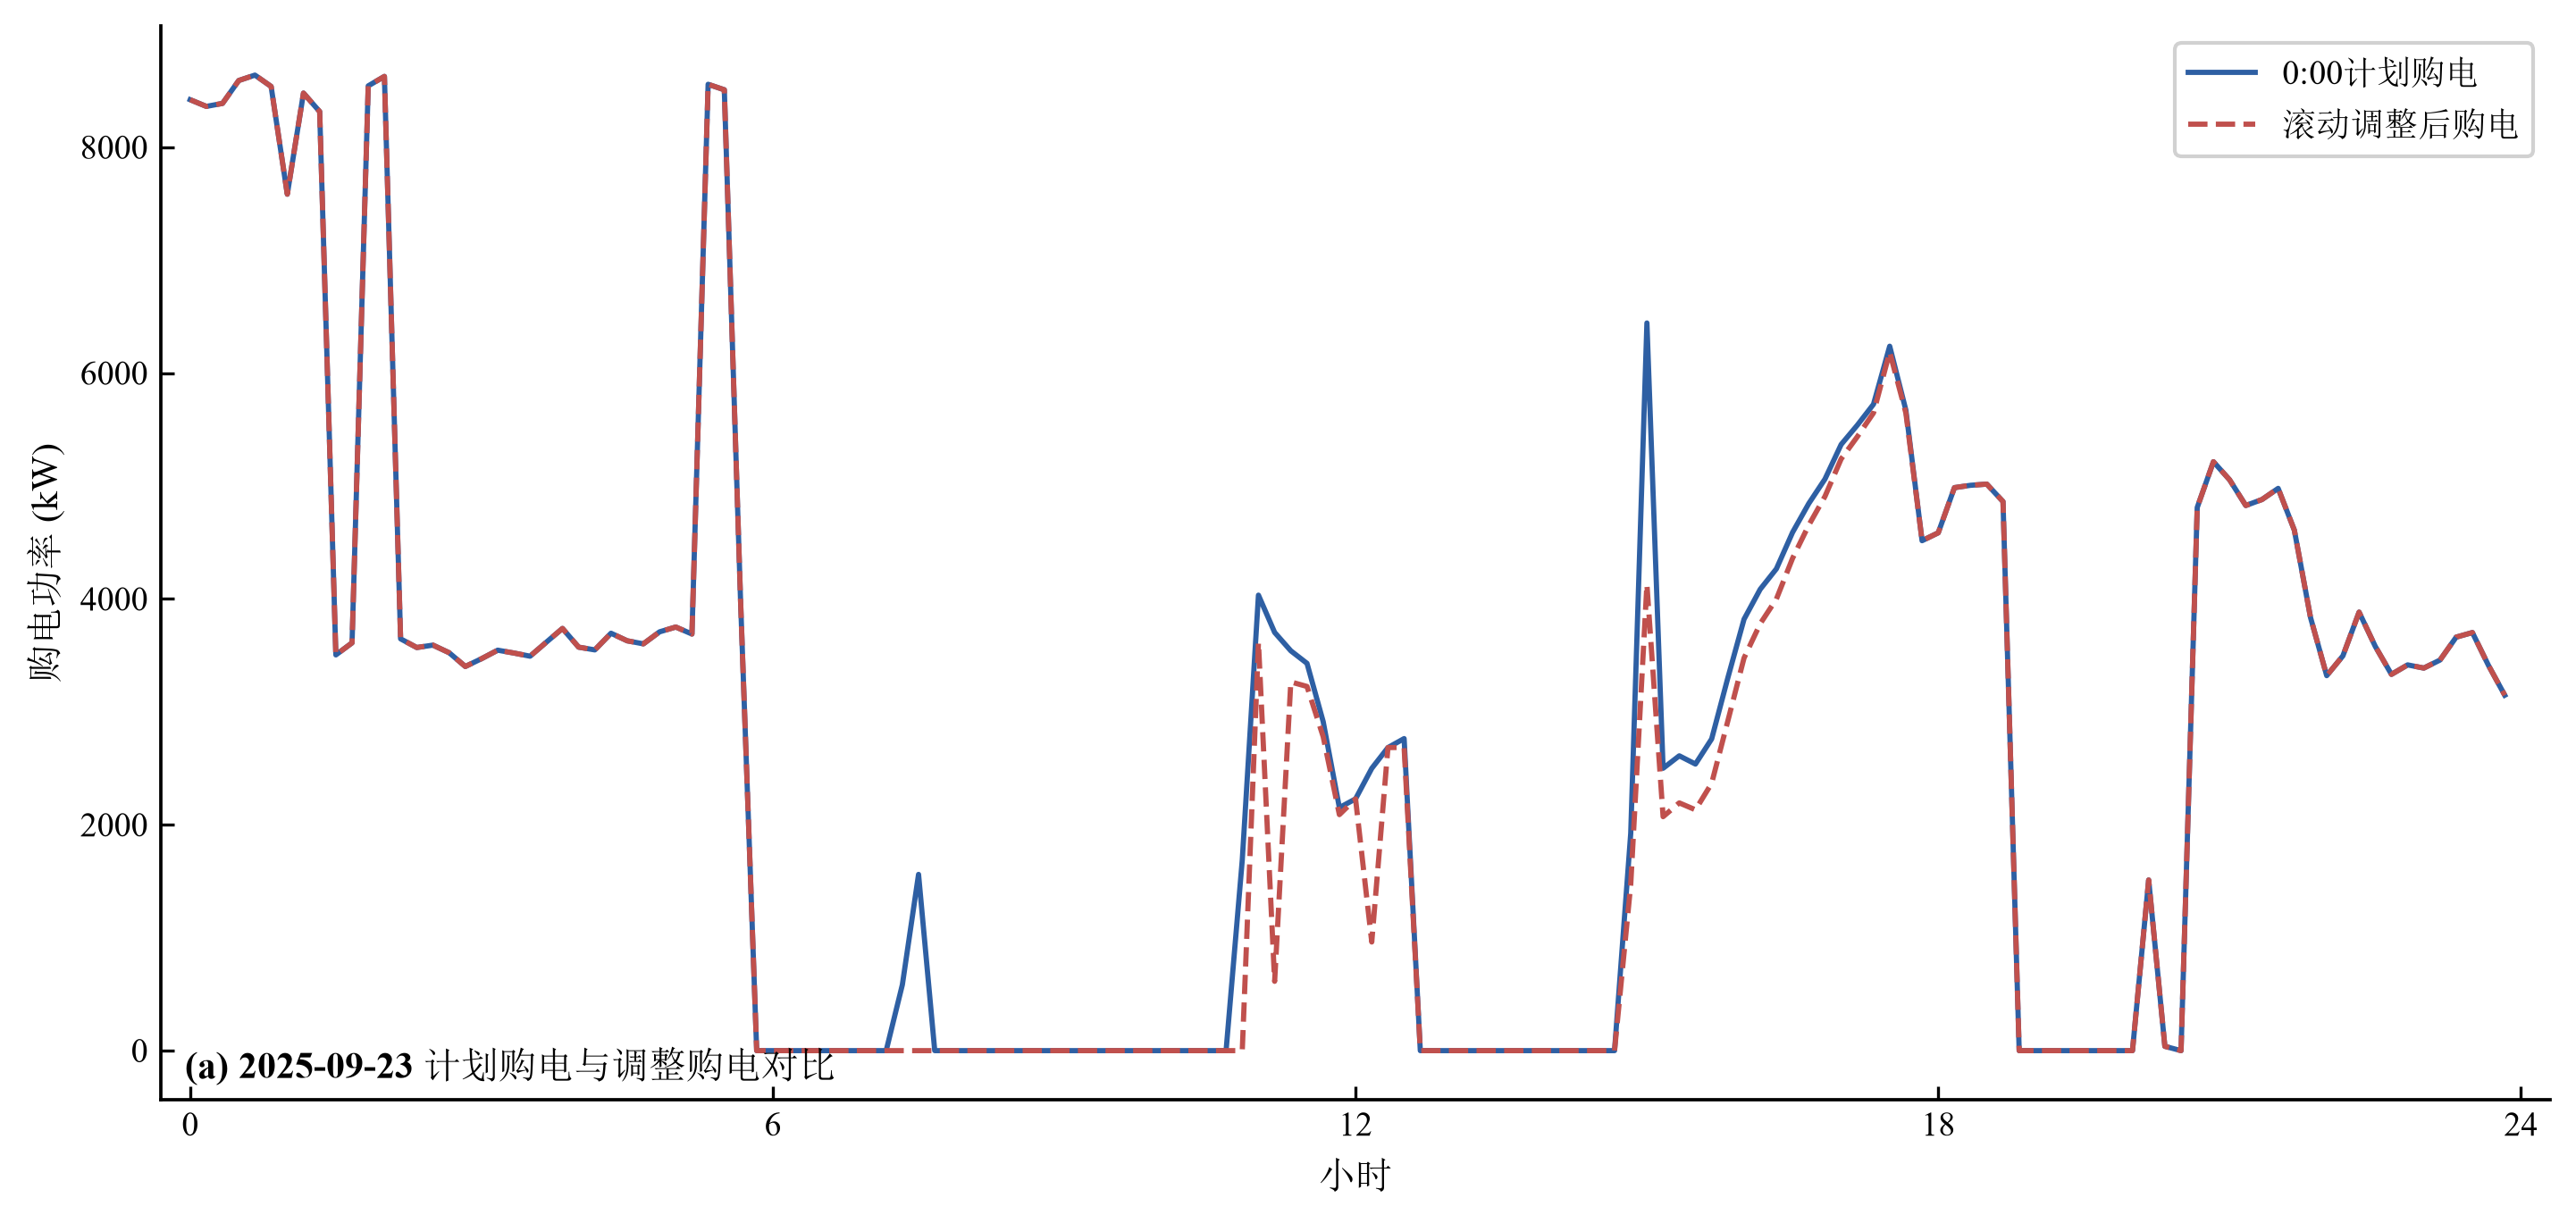
\includegraphics[width=0.70\textwidth]{求解/问题三/图片/图3-2_计划与调整购电量对比.png}
    \caption{典型日计划购电与调整购电功率对比}
    \label{fig:结果3-2}
\end{figure}

由调整后策略生成的 2.1—12.31 逐日紧急购电量如图\ref{fig:结果3-3}所示。紧急购电量在多数日期维持在较低水平，仅在实际供电出现缺口的个别日期出现尖峰，说明滚动调整已有效吸收了大部分预报误差，使实际供电缺口显著缩小。

\begin{figure}[H]
    \centering
    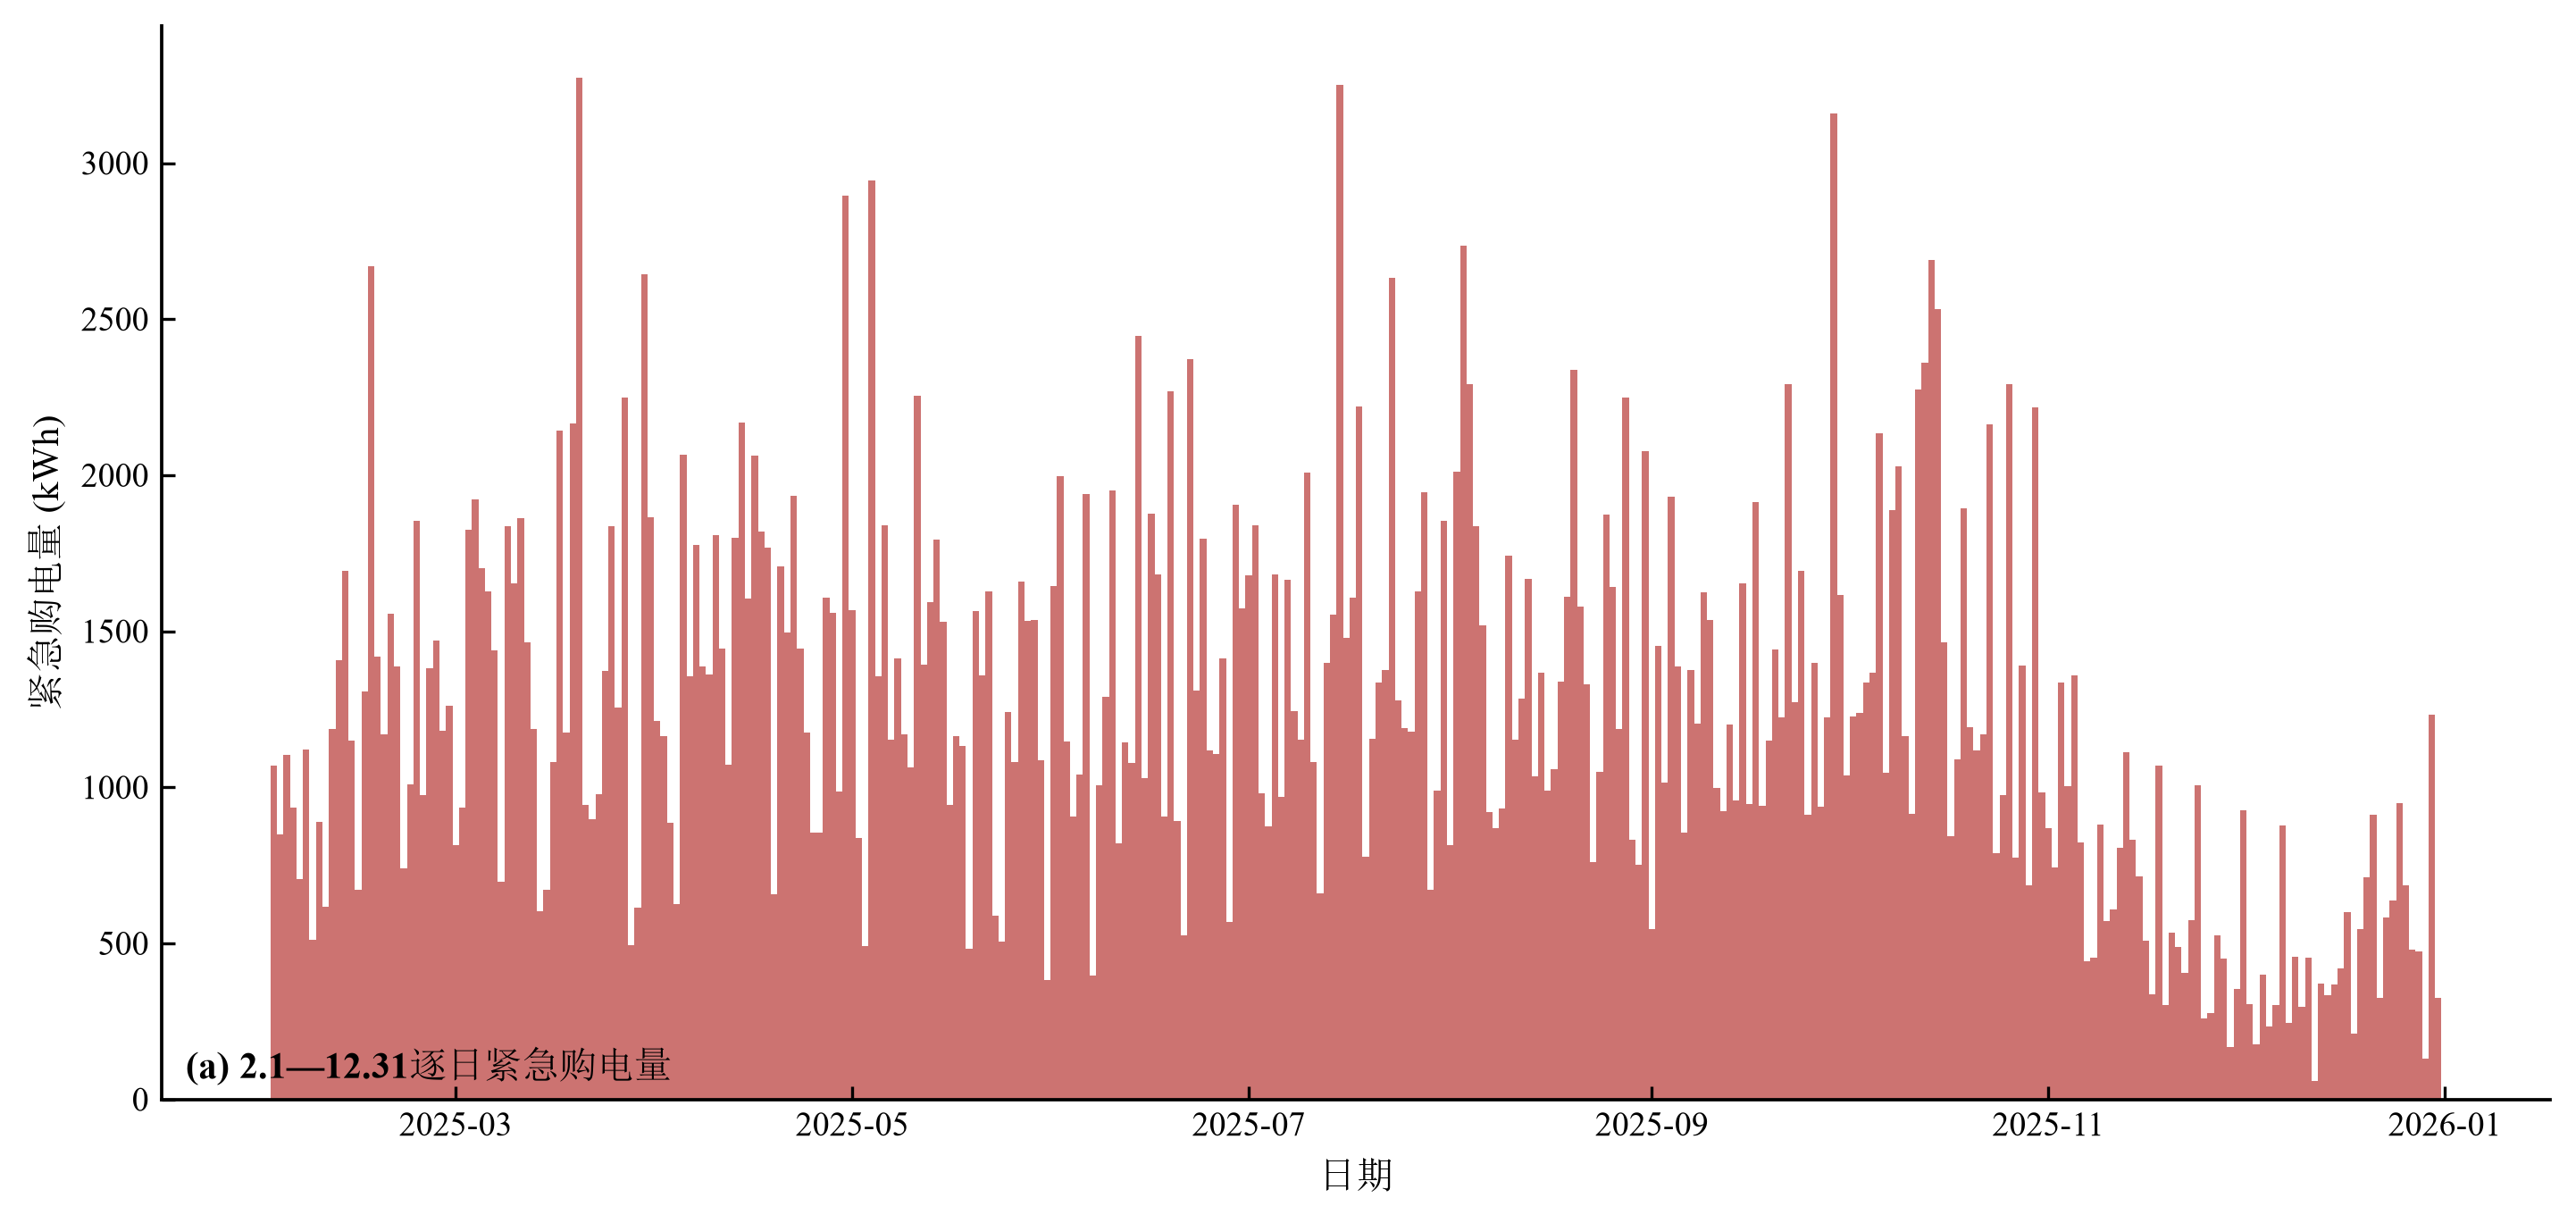
\includegraphics[width=0.70\textwidth]{求解/问题三/图片/图3-3_全年紧急购电量.png}
    \caption{2.1—12.31逐日紧急购电量}
    \label{fig:结果3-3}
\end{figure}

有无调整的费用对比与月度节省如图\ref{fig:结果3-4}所示。引入滚动调整后，总费用由 14782072.51 元降至 14337999.15 元，各月均有不同程度的费用节省，说明利用 6:00、12:00、18:00 的新预报进行购电调整具有明确的经济收益。

\begin{figure}[H]
    \centering
    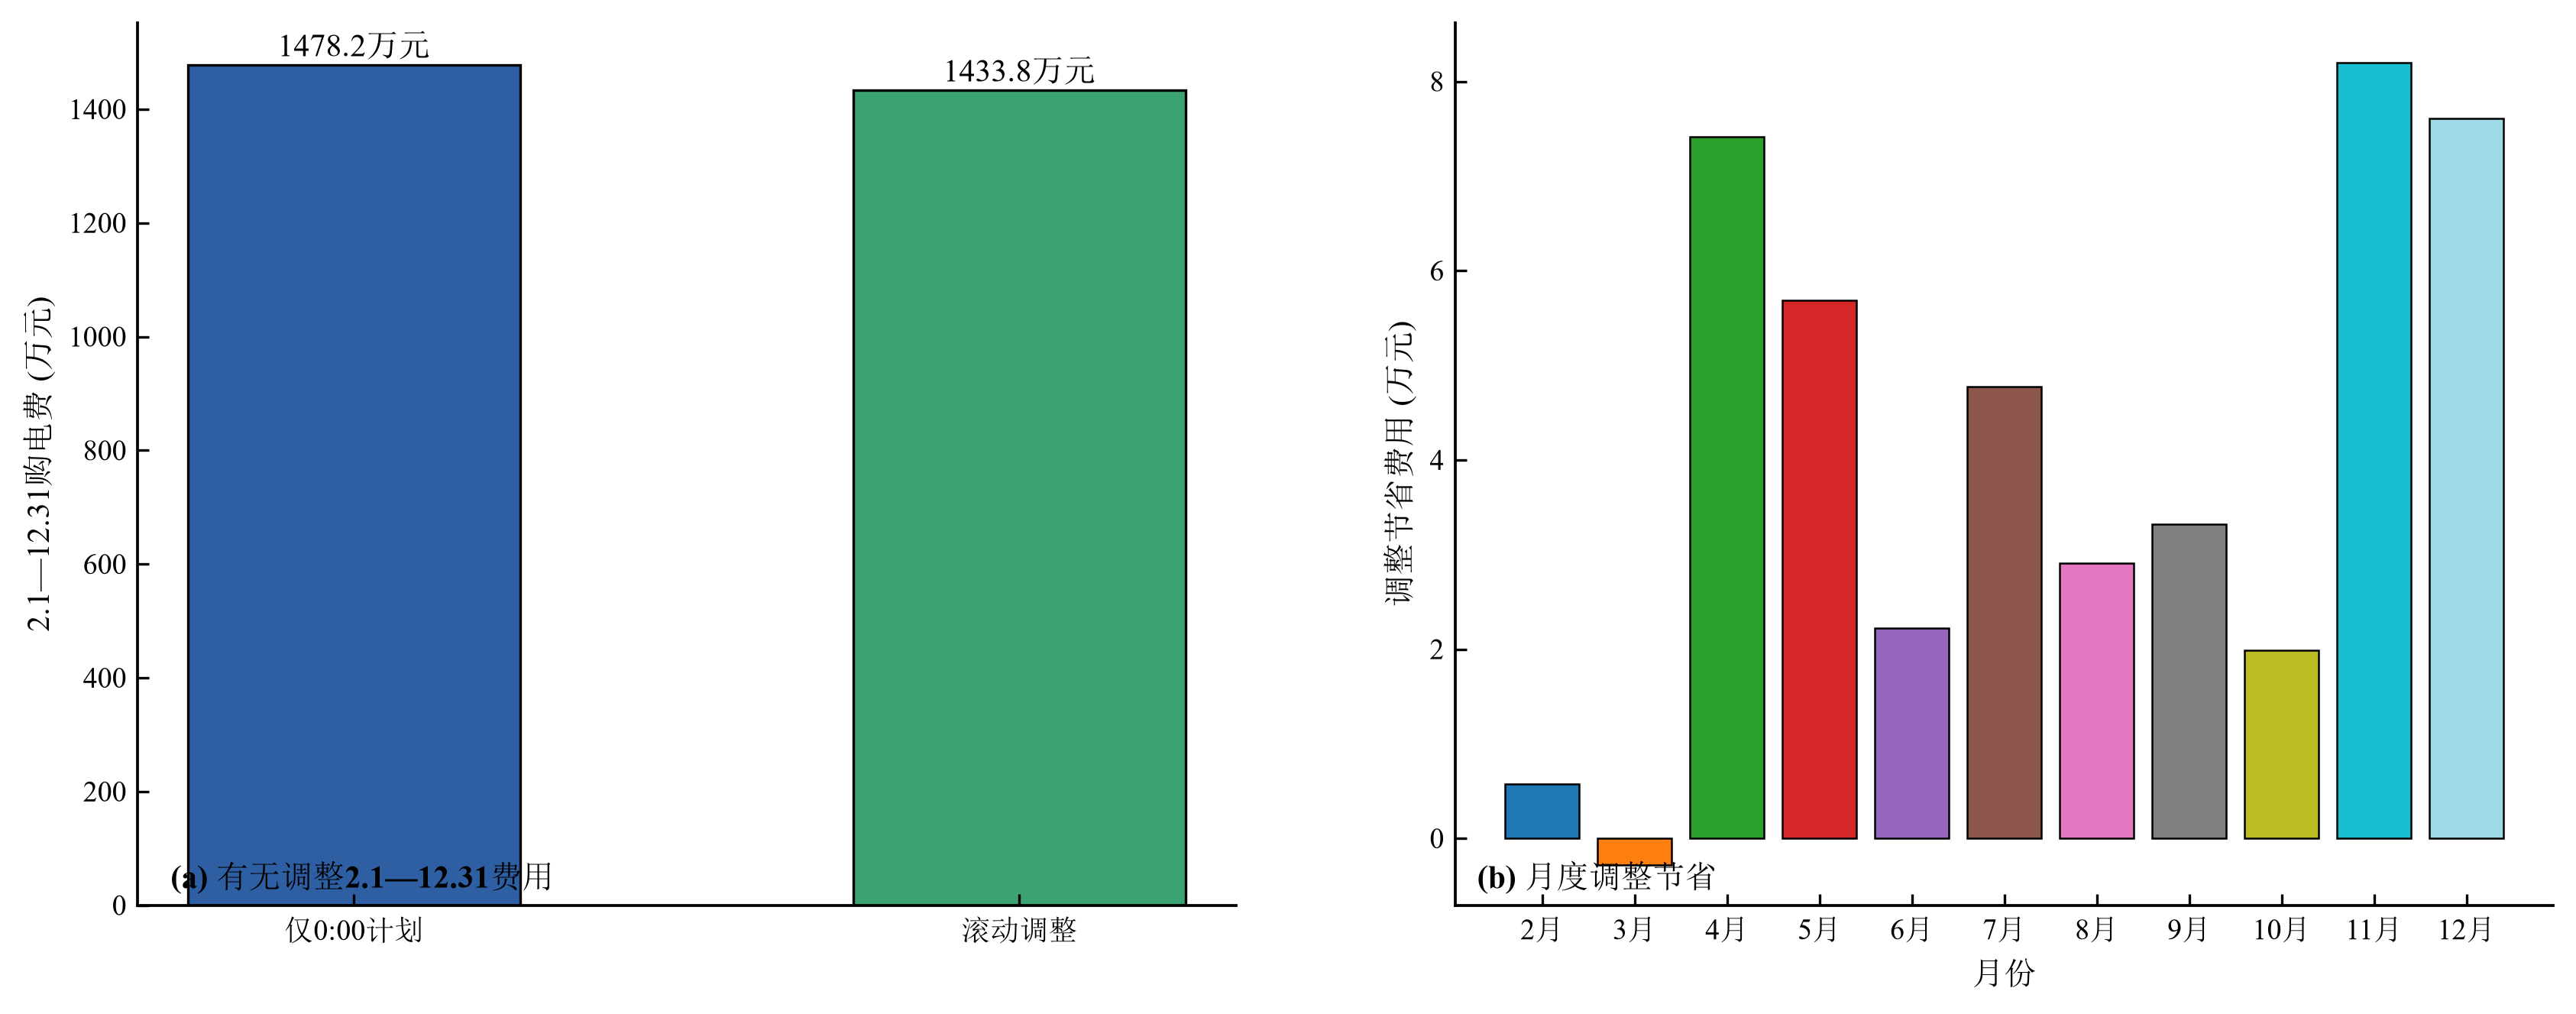
\includegraphics[width=0.72\textwidth]{求解/问题三/图片/图3-4_有无调整费用对比.png}
    \caption{有无滚动调整的费用对比与月度节省（2.1—12.31）}
    \label{fig:结果3-4}
\end{figure}

典型日的储能荷电状态在计划与调整后两种策略下的对比如图\ref{fig:结果3-5}所示。调整后储能充放电轨迹随更新预报自适应变化，荷电状态全程维持在约束区间内，且 0:00 与 24:00 的储电量仍保持合理衔接，说明调整策略在提升经济性的同时未破坏储能的运行约束。

\begin{figure}[H]
    \centering
    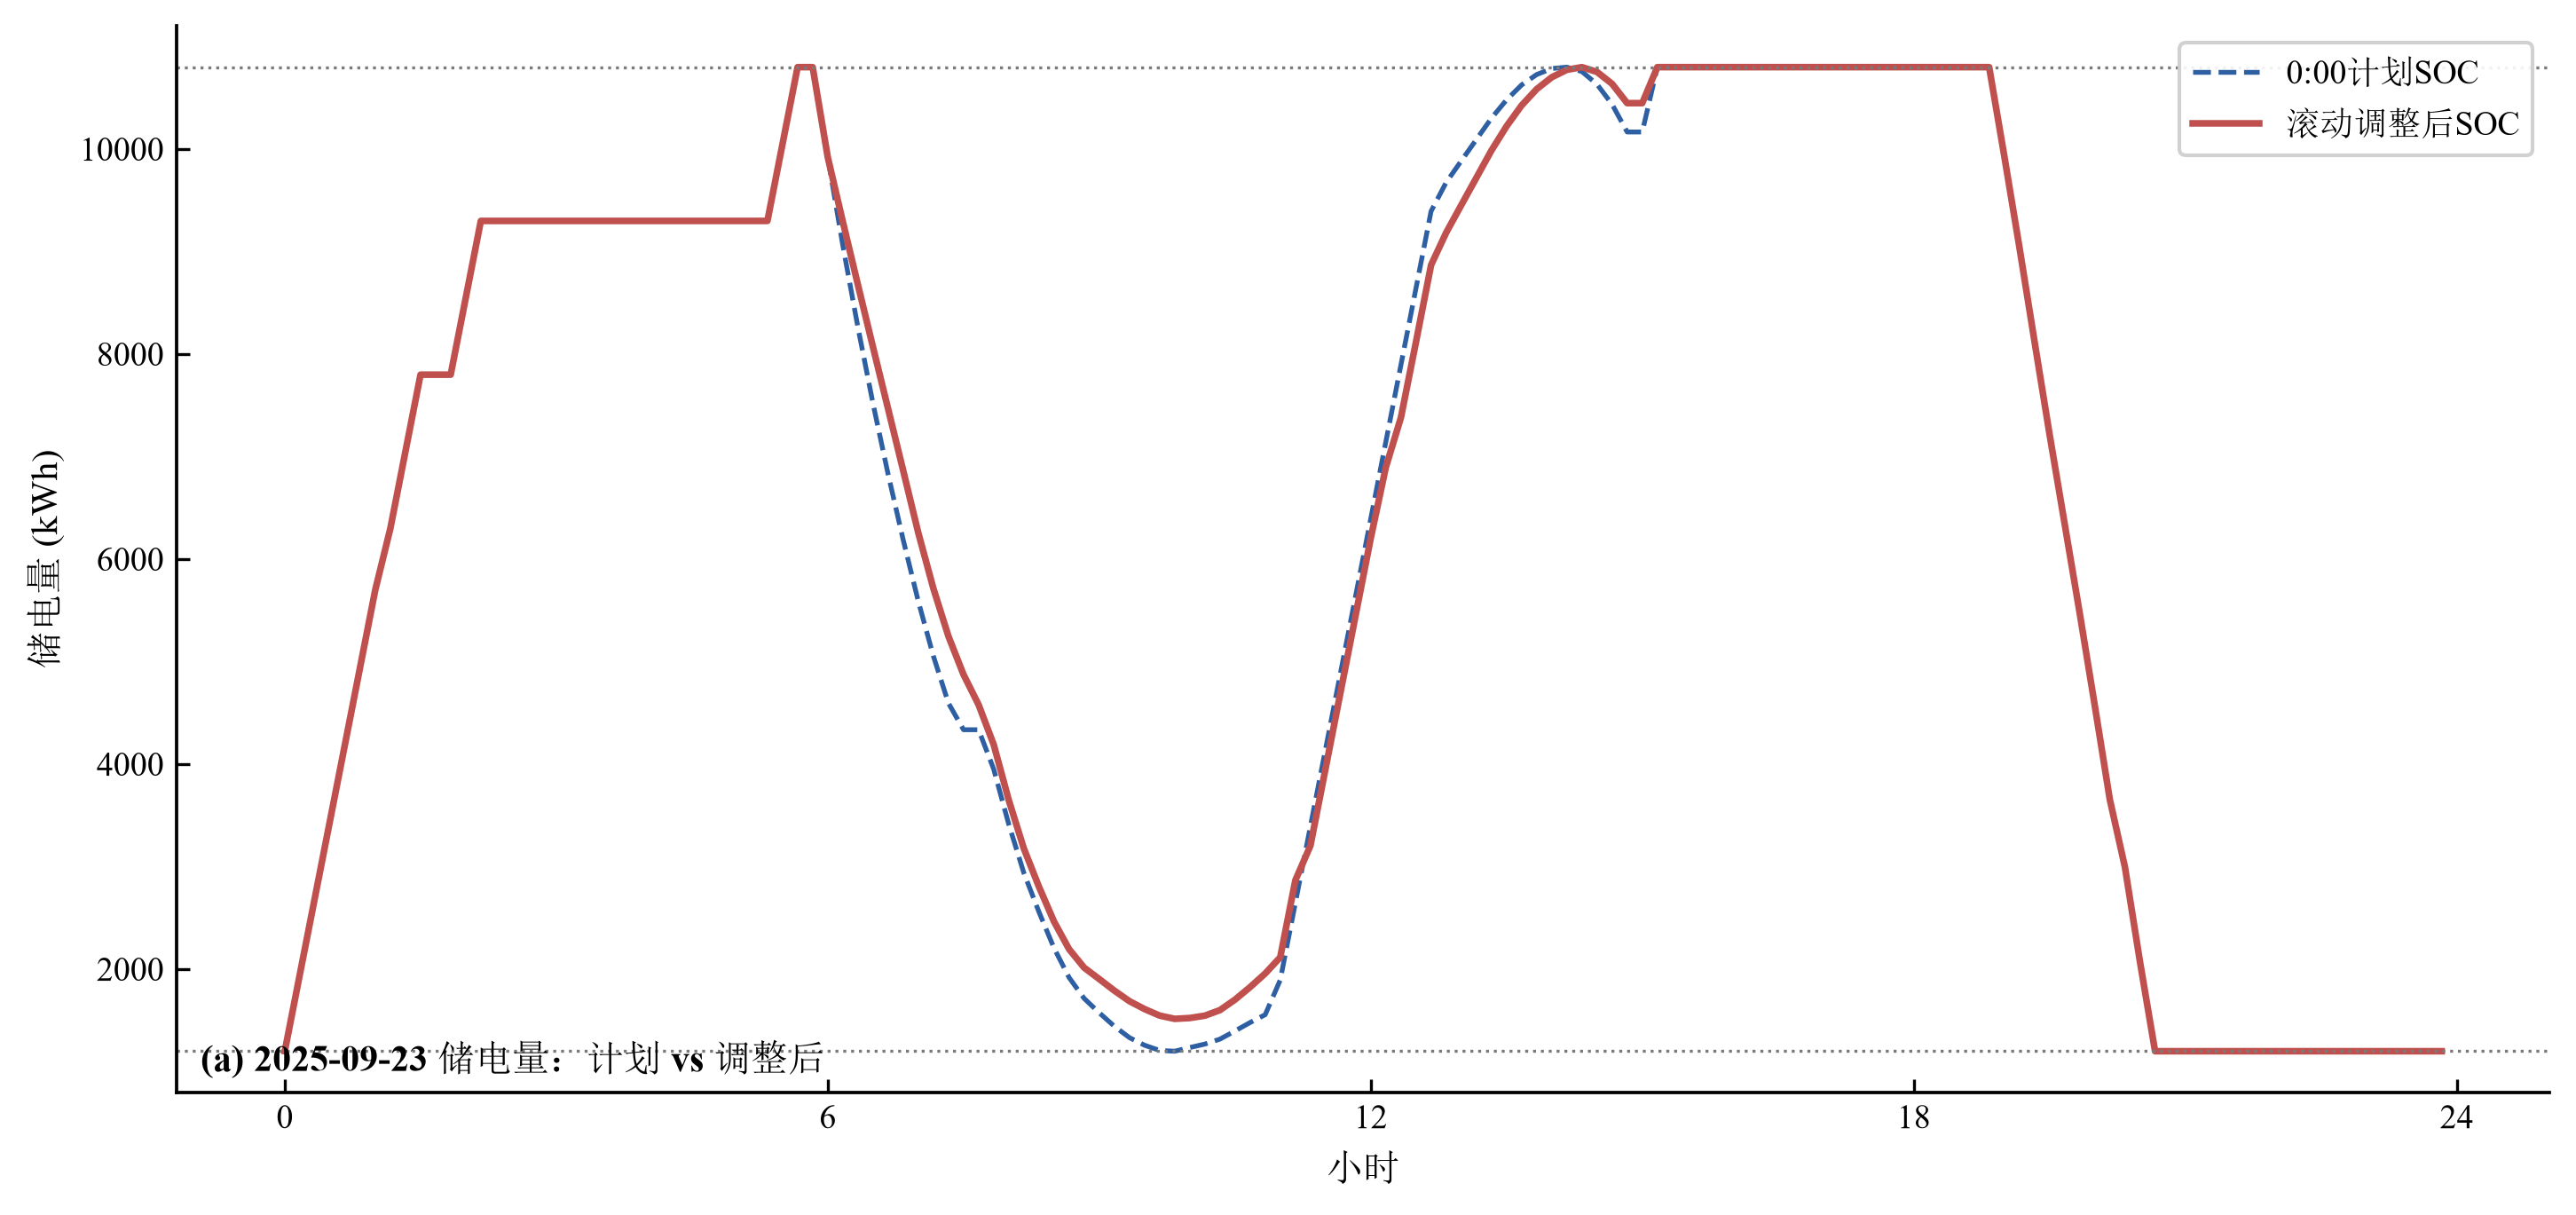
\includegraphics[width=0.70\textwidth]{求解/问题三/图片/图3-5_计划与调整后SOC对比.png}
    \caption{典型日计划与调整后储能荷电状态对比}
    \label{fig:结果3-5}
\end{figure}

2—12 月费用的月度构成如图\ref{fig:结果3-6}所示，计划购电费用占主导，调整相关费用与紧急购电费用占比相对较小，且冬季总费用最高、夏季最低，与负荷和光伏的季节特性一致。

\begin{figure}[H]
    \centering
    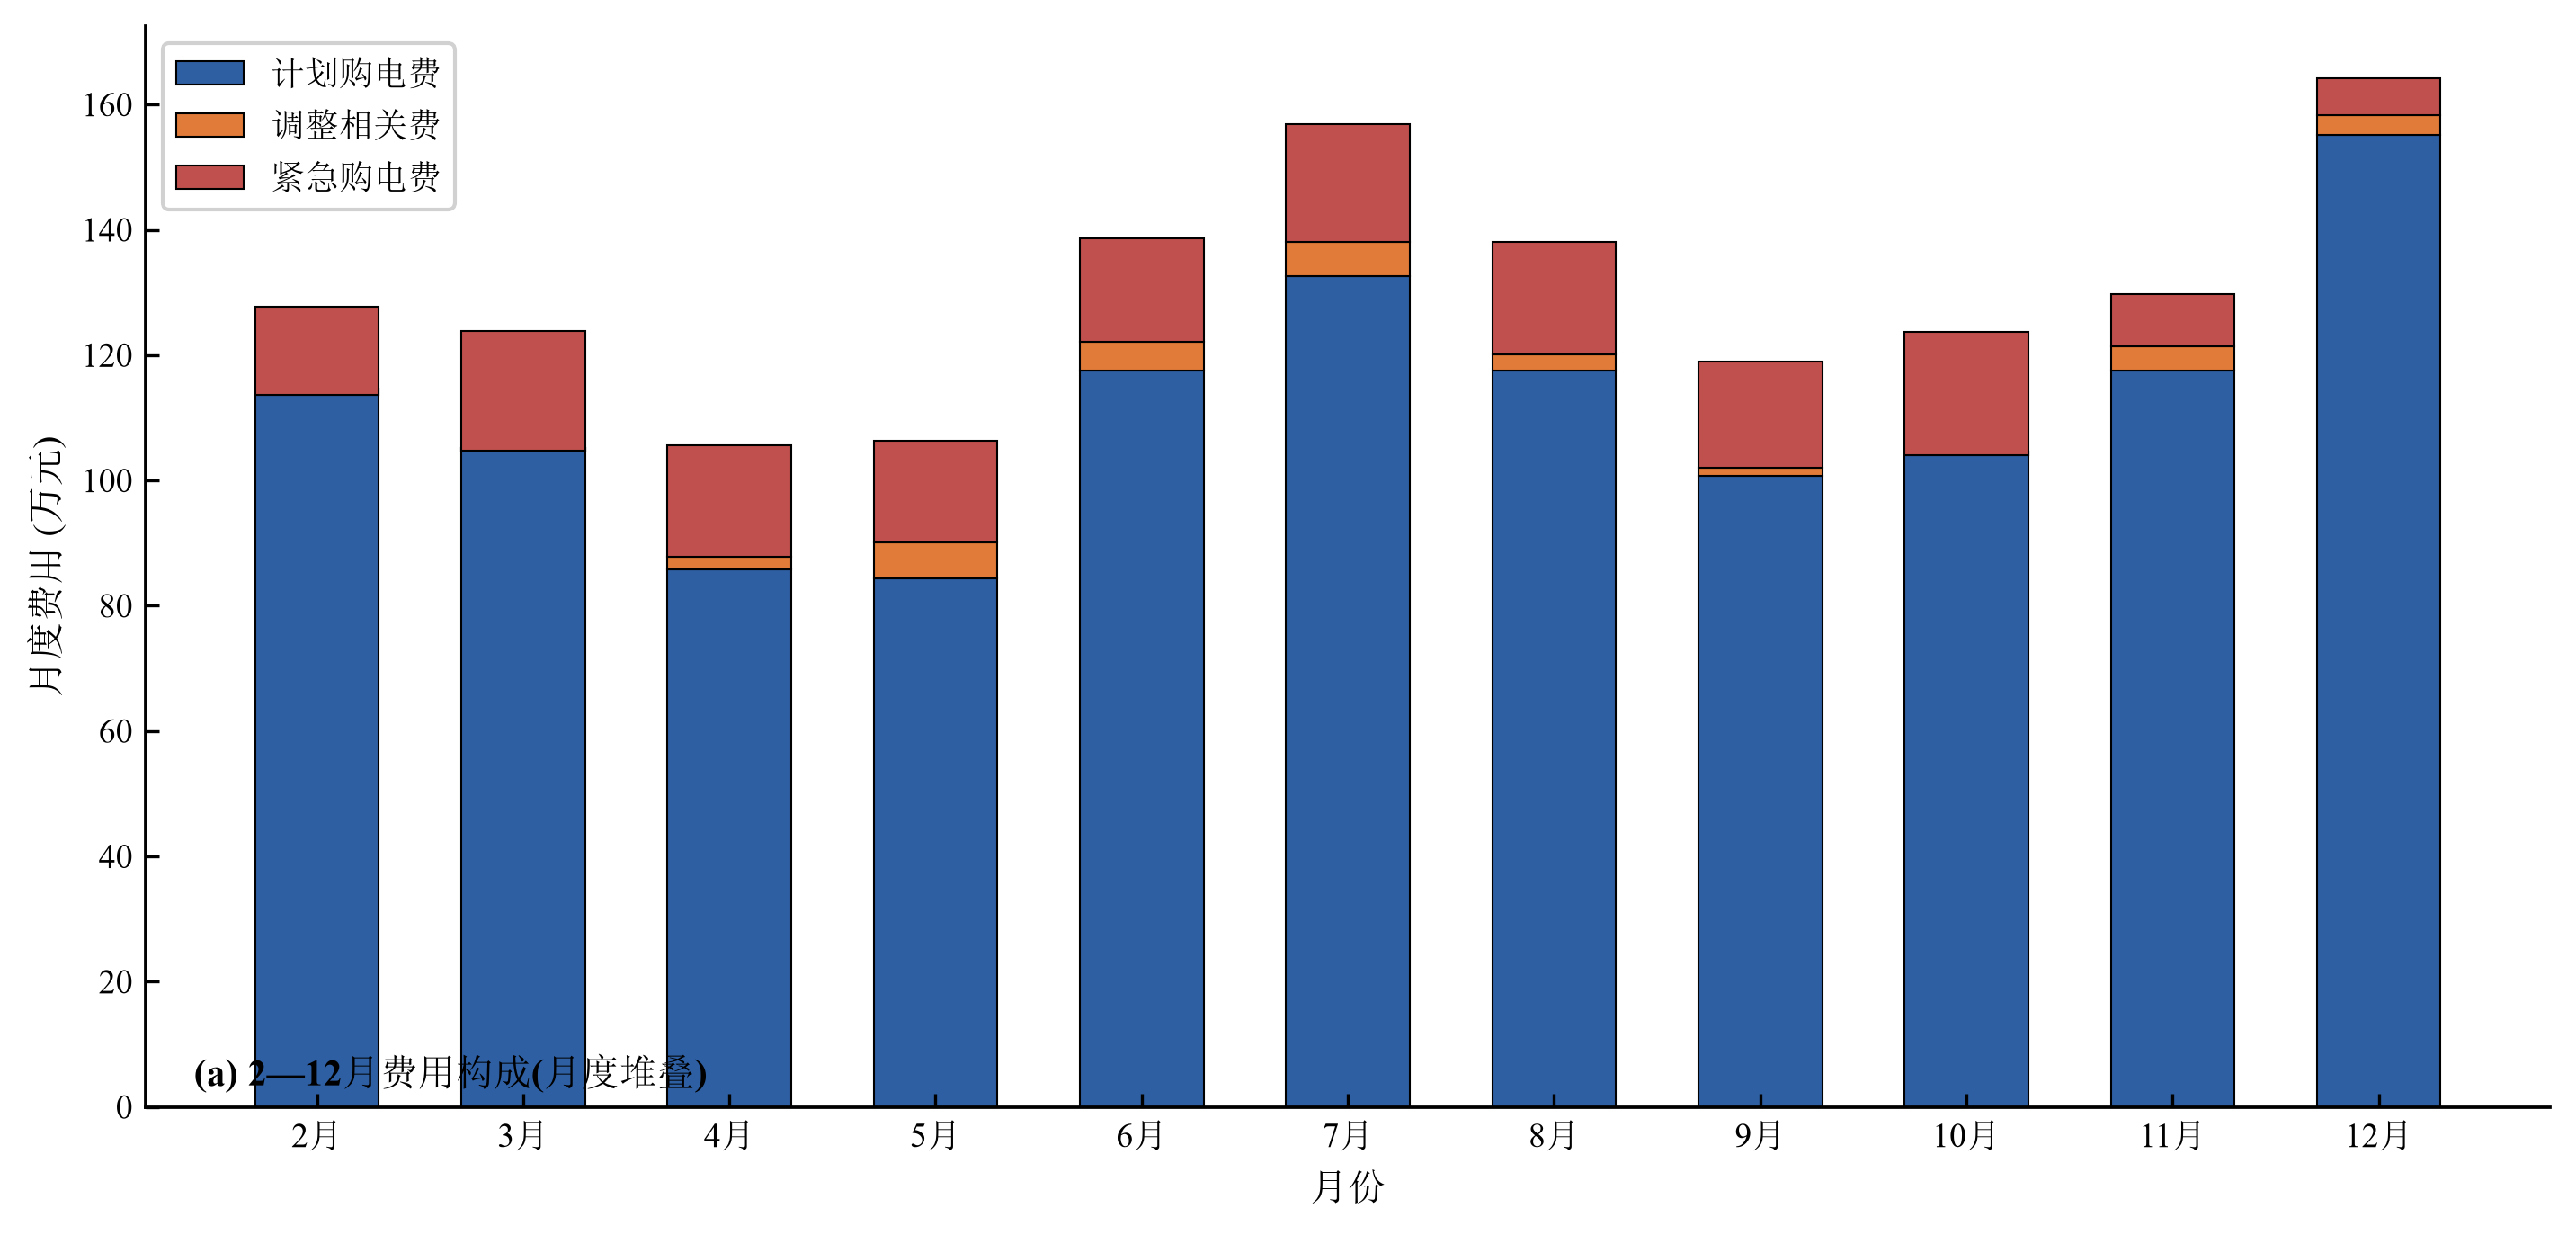
\includegraphics[width=0.70\textwidth]{求解/问题三/图片/图3-6_全年费用构成.png}
    \caption{2.1—12.31费用月度构成}
    \label{fig:结果3-6}
\end{figure}

为完整回答“是否需要引入其他时刻的预报”这一问，本文在 0/6/12/18 方案基础上进一步做了两类边际收益分析（口径均为 2 月 1 日—12 月 31 日）。第一类为逐次累加题目给定的真实预报时刻：仅用 0:00 计划时费用为 14782072.51 元；依次引入 6:00、12:00、18:00 调整后，费用分别变为 14819461.95 元、14357950.79 元与 14337999.15 元，三个时刻的边际节省分别为 $-3.74$ 万元、$46.15$ 万元与 $2.00$ 万元，其中 12:00 预报的价值最为突出（6:00 预报单独引入时边际收益略为负值，说明并非所有新增预报时刻都具有正收益）。第二类为“加密更多时刻”的上界分析：由于附件三只提供 0:00、6:00、12:00、18:00 四个时刻的预报，本文以“各时刻预报完全准确（完全预见）”作为最乐观假设，考察把调整间隔由 6 小时加密到 3 小时、1 小时，以及在 6 小时方案中增加 9:00、15:00 时刻的额外收益，结果如图\ref{fig:结果3-7}所示。

\begin{figure}[H]
    \centering
    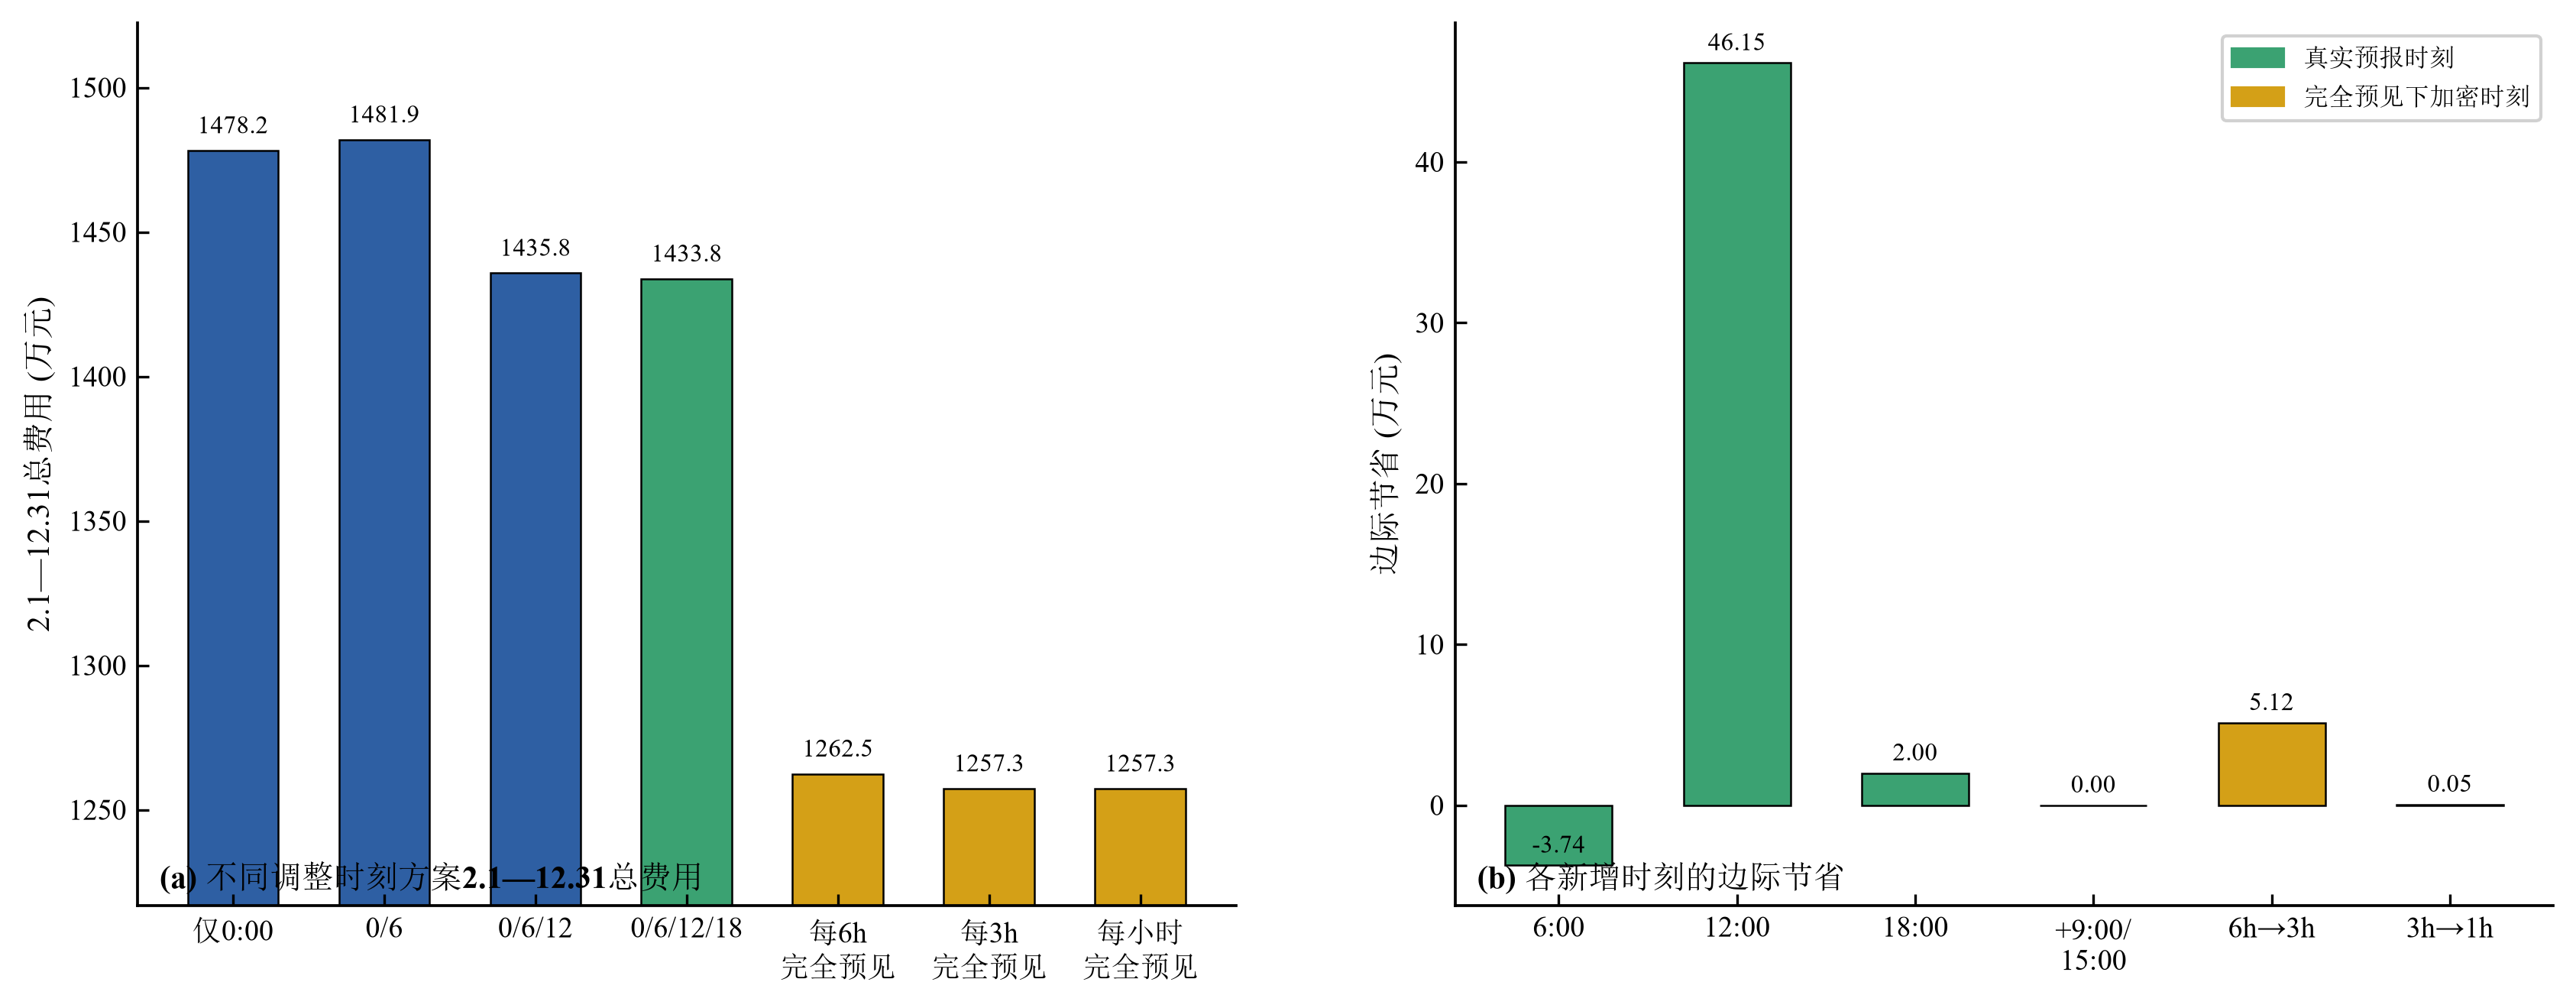
\includegraphics[width=0.85\textwidth]{求解/问题三/图片/图3-7_其他时刻预报边际收益.png}
    \caption{不同调整时刻方案的总费用与各新增时刻的边际节省（2.1—12.31）}
    \label{fig:结果3-7}
\end{figure}

在完全预见下，6 小时间隔已几乎捕获全部频率收益：把间隔进一步加密到 3 小时、1 小时仅分别再节省 5.12 万元与 0.05 万元，而在 6 小时方案中增加 9:00、15:00 时刻的边际收益为 0；与之相对，若保持 6 小时间隔不变、仅把 6/12/18 的真实预报替换为完全预见，费用还可再降 171.33 万元。这说明未实现的节省潜力主要来自光伏预报精度而非调整频率。

综合以上结果：引入 6:00、12:00、18:00 的预报制定调整购电策略是必要的，可使购电费用较仅用 0:00 计划降低约 3.00\%；但进一步引入更多预报时刻（如每小时、每 3 小时，或增加 9:00、15:00 等）并无必要——即使在完全预见的最乐观假设下，加密调整间隔的边际收益也趋近于零（0.05 万～5.12 万元量级）。因此，若需进一步降低购电费用，应优先提高各预报时刻的预报精度，而非增加预报时刻数量。



% ════════════════════════════════════════════
% 单个问题的建立求解（5.4.问题四.tex，二级标题包装）
% ════════════════════════════════════════════
\subsection{问题四的模型的建立和求解}


% ════════════════════════════════════════════
% 具体分析（5.4.1.具体分析.tex，三级子块）
% ════════════════════════════════════════════
\subsubsection{具体分析}

针对问题四，本问属于波动电价下的随机调度优化类问题，在问题二、问题三模型的基础上，将固定的分时电价替换为附件四提供的实时波动电价，重新计算逐日计划购电与滚动调整购电策略。

本文先读取附件四中全年 365 天、每天 144 个 10 分钟时间点的波动电价数据，与附件二的实际负载光伏、附件三的光伏预报完成时间对齐；将问题二、问题三模型中的电价参数替换为逐间隔波动电价，重新求解逐日线性规划与滚动调整线性规划；分别得到波动电价下问题二的计划购电策略与问题三的调整购电策略；最后与固定电价结果进行对比，分析电价波动对微网购电费用的影响。具体分析流程如图\ref{fig:analysis4_flow}所示。

\begin{figure}[H]
    \begin{center}
        \begin{tikzpicture}[x=1cm, y=0.75cm,
            flowhead/.style={rectangle, rounded corners=3pt, draw=violet!70!black, fill=violet!50!black, text=white, font=\bfseries, minimum width=7.2cm, minimum height=1.1cm, align=center, inner sep=2pt, line width=0.7pt},
            flowbox/.style={rectangle, rounded corners=2.5pt, draw=violet!65!black, fill=violet!14, minimum width=7.2cm, minimum height=1.0cm, align=center, inner sep=2pt, line width=0.6pt},
            flowend/.style={rectangle, rounded corners=2.5pt, draw=violet!75!black, fill=violet!40!black, text=white, font=\bfseries, minimum width=7.2cm, minimum height=1.0cm, align=center, inner sep=2pt, line width=0.7pt},
            flowarrow/.style={thick, -{Stealth}, violet!55!black}
        ]
            \node[flowhead] at (0, 0) (h) {问题四：波动电价购电策略};
            \node[flowbox] at (0, -1.8) (s1) {\textbf{读取波动电价}\\\footnotesize 全年 365 天 × 144 点波动电价};
            \node[flowbox] at (0, -3.6) (s2) {\textbf{数据时间对齐}\\\footnotesize 与负荷 · 光伏 · 预报对齐};
            \node[flowbox] at (0, -5.4) (s3) {\textbf{替换电价参数}\\\footnotesize 逐间隔替换为波动电价};
            \node[flowbox] at (0, -7.2) (s4) {\textbf{重算问题二}\\\footnotesize 得到波动电价下逐日计划购电};
            \node[flowbox] at (0, -9.0) (s5) {\textbf{重算问题三}\\\footnotesize 得到波动电价下滚动调整购电};
            \node[flowbox] at (0, -10.8) (s6) {\textbf{惩罚与紧急计价}\\\footnotesize 分段惩罚与 5 倍紧急购电};
            \node[flowbox] at (0, -12.6) (s7) {\textbf{固定波动对比}\\\footnotesize 固定电价与波动电价费用对比};
            \node[flowend] at (0, -14.4) (s8) {电价影响分析\\\footnotesize 分析电价波动对购电费用的影响};
            \draw[flowarrow] (h) -- (s1);
            \draw[flowarrow] (s1) -- (s2);
            \draw[flowarrow] (s2) -- (s3);
            \draw[flowarrow] (s3) -- (s4);
            \draw[flowarrow] (s4) -- (s5);
            \draw[flowarrow] (s5) -- (s6);
            \draw[flowarrow] (s6) -- (s7);
            \draw[flowarrow] (s7) -- (s8);
        \end{tikzpicture}
        \caption{问题四分析流程图}
        \label{fig:analysis4_flow}
    \end{center}
\end{figure}


% ════════════════════════════════════════════
% 模型准备（5.4.2.模型准备.tex，三级子块）
% ════════════════════════════════════════════
\subsubsection{模型准备}

\textbf{1.数据预处理}

附件四提供了 2025 年全年每天不同时刻的外网实时波动电价，时间分辨率为 10 分钟。设第 $d$ 天第 $k$ 个间隔的波动电价为 $p_{d,k}$，则全年电价数据可组织为：
\begin{equation}
    \boldsymbol{P}=[p_{d,k}]_{365\times 144}
\end{equation}
对其进行数值化检查，全年无缺失值，电价分布范围约为 $0.3\sim 1.6$ 元/kWh。波动电价与固定电价的典型日对比如图\ref{fig:preprocess4}所示。

\begin{figure}[H]
    \centering
    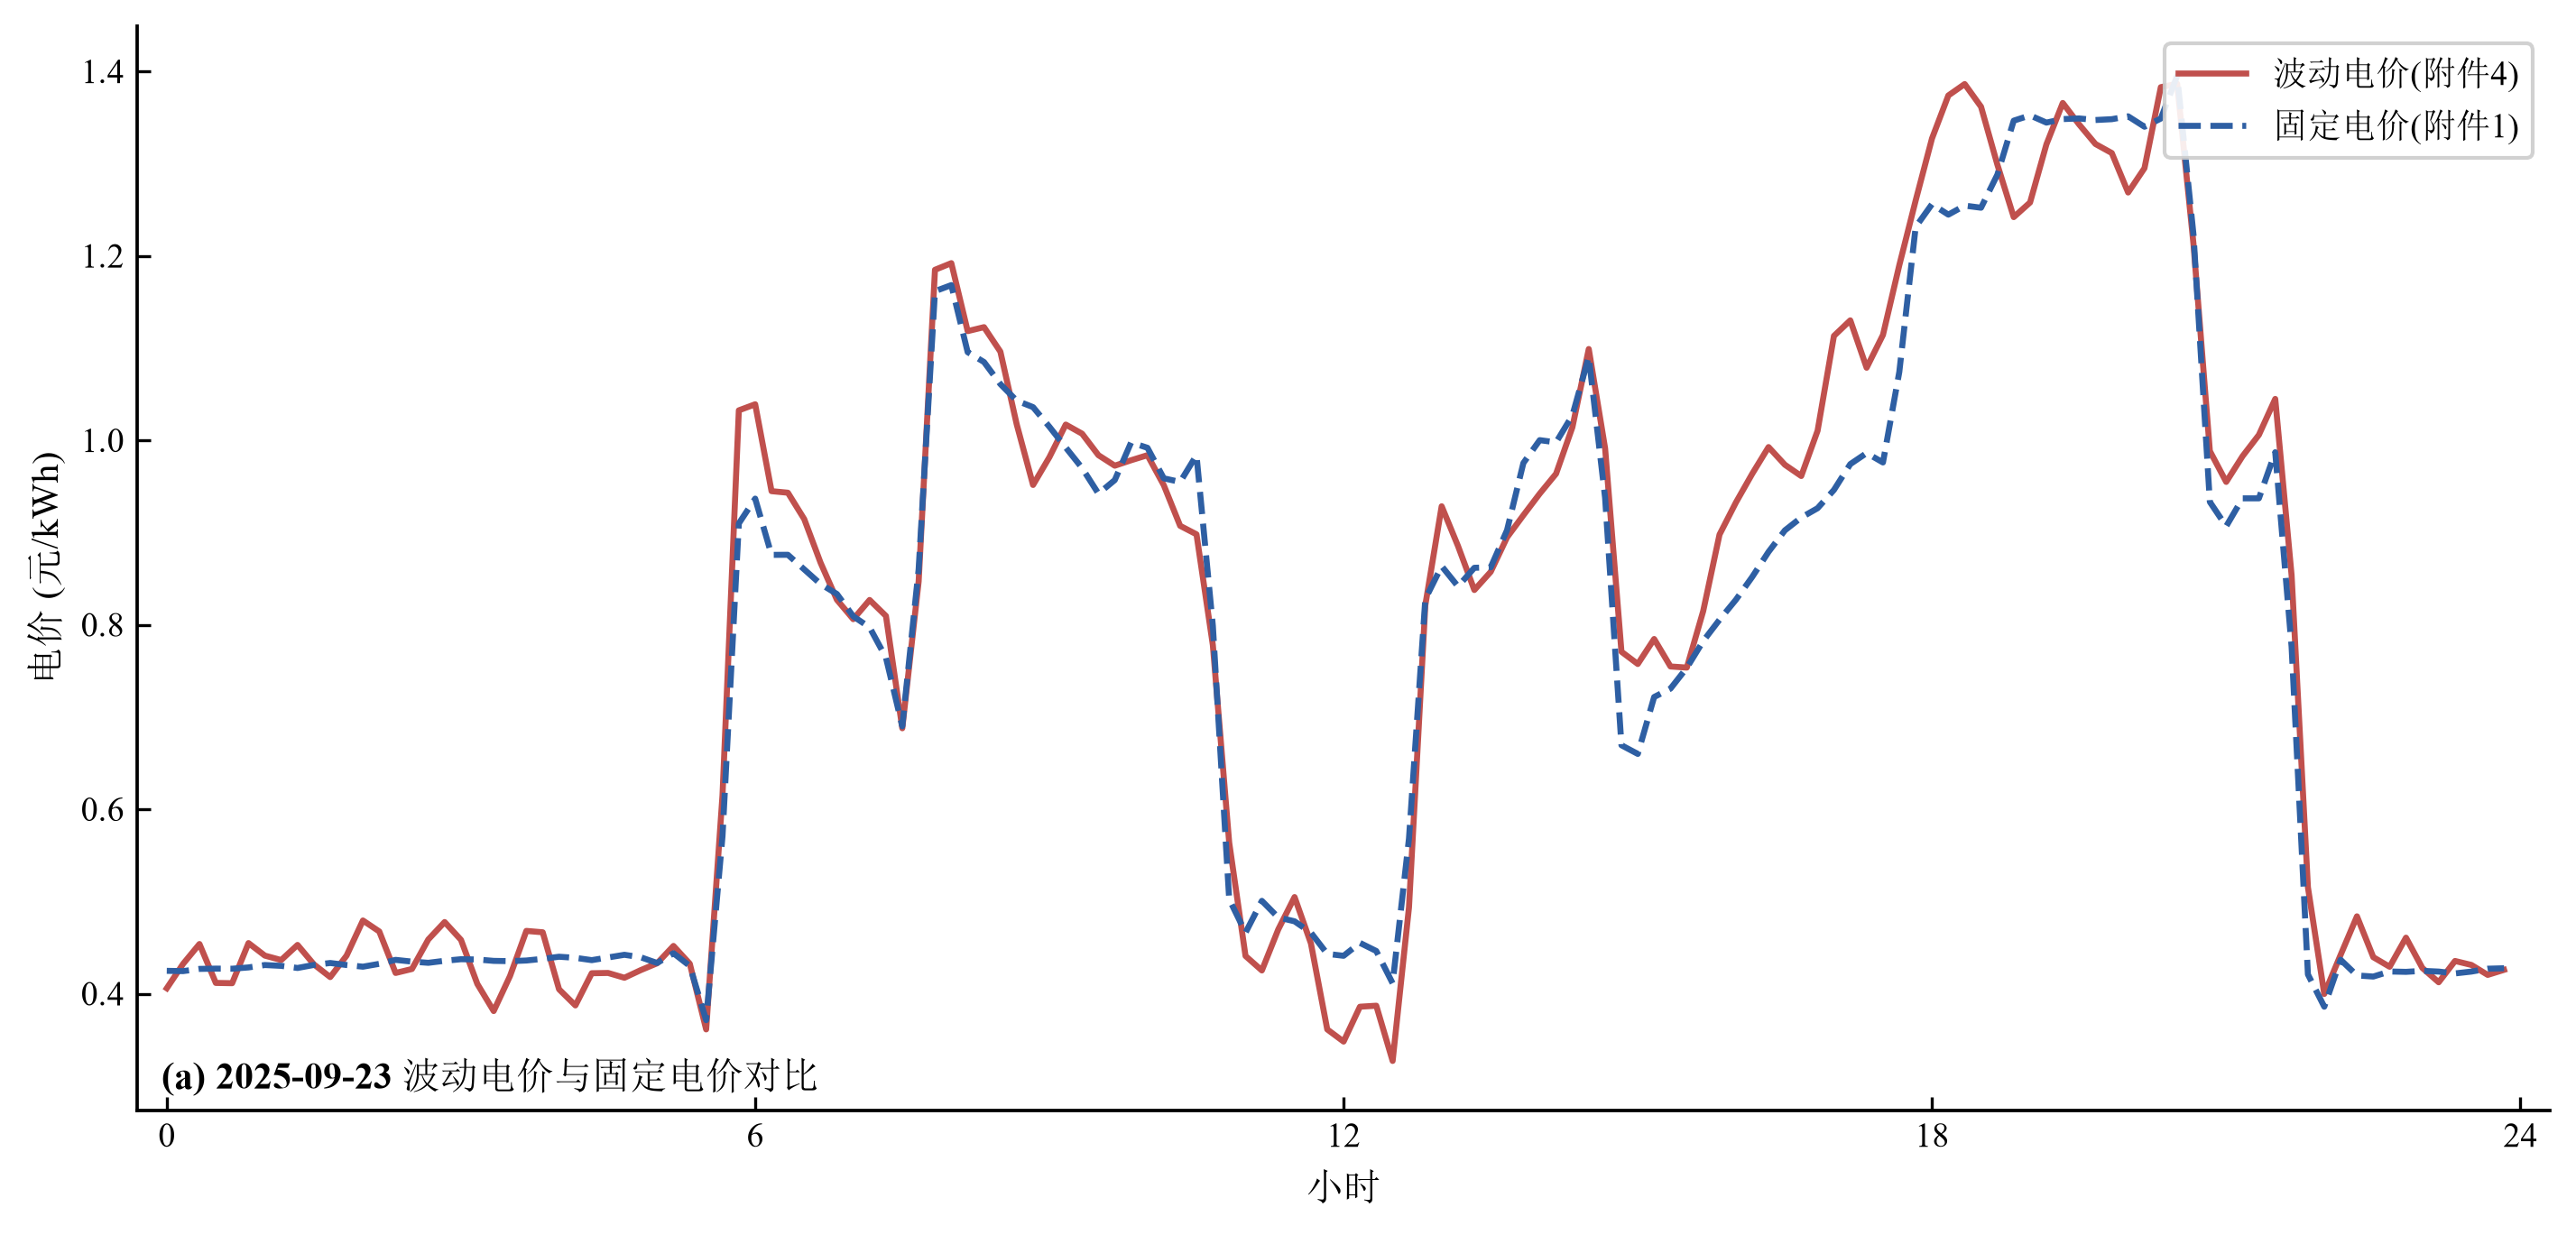
\includegraphics[width=0.70\textwidth]{求解/问题四/图片/图4-1_波动与固定电价对比.png}
    \caption{波动电价与固定电价的典型日对比}
    \label{fig:preprocess4}
\end{figure}

由图\ref{fig:preprocess4}可知，波动电价在同一天内剧烈起伏，白天用电高峰电价可达 1.5 元/kWh 以上，夜间低谷可低至 0.35 元/kWh 左右，其峰谷价差明显大于固定电价，因此储能低充高放的套利空间更大，但购电时机的把握也更为关键。

\textbf{2.算法选择}

在完成电价数据预处理后，本问的建模框架与问题二、问题三完全一致，仅将电价参数由固定序列替换为逐间隔波动序列。由于目标函数与约束仍是线性的，问题二对应部分可继续采用逐日线性规划，问题三对应部分可继续采用滚动线性规划，算法选择与前述问题一致，此处不再重复对比，仅对参数替换作说明：将式(1)中的 $p_k$ 替换为 $p_{d,k}$ 即可得到波动电价下的模型。


% ════════════════════════════════════════════
% 模型建立（5.4.3.模型建立.tex，三级子块）
% ════════════════════════════════════════════
\subsubsection{模型建立}

针对问题四，本节在问题二、问题三模型的基础上，将固定分时电价替换为逐间隔波动电价，建立波动电价下的微网购电策略模型。具体过程如下。

\textbf{步骤1：波动电价下的逐日计划模型}

对应问题二，第 $d$ 天的逐日计划购电模型的目标函数为：
\begin{equation}
    \min \; Z_d=\sum_{k=0}^{143} g_{d,k}\,p_{d,k}\,\Delta t
\end{equation}
功率平衡、储能状态递推、容量与功率约束分别保持为：
\begin{equation}
    g_{d,k}+S_{d,k}+d_{d,k}-c_{d,k}\geq L_{d,k}
\end{equation}
\begin{equation}
    E_{d,k+1}=E_{d,k}+\eta\,c_{d,k}\,\Delta t-\frac{1}{\eta}\,d_{d,k}\,\Delta t
\end{equation}
\begin{equation}
    E_{\min}\leq E_{d,k}\leq E_{\max},\quad 0\leq c_{d,k},d_{d,k}\leq P_{\max},\quad g_{d,k}\geq 0
\end{equation}
日间储电量传递关系与首日初值同问题二：
\begin{equation}
    E_{d+1,0}=E_{d,144},\quad E_{0,0}=6000
\end{equation}

\textbf{步骤2：波动电价下的滚动调整模型}

对应问题三，0:00 计划购电的目标函数与约束为：
\begin{equation}
    \min \; Z^{\mathrm{p}}=\sum_{k=0}^{143} g^{\mathrm{p}}_k\,p_{d,k}\,\Delta t
\end{equation}
\begin{equation}
    g^{\mathrm{p}}_k+S^{0}_k+d^{\mathrm{p}}_k-c^{\mathrm{p}}_k\geq L_k
\end{equation}
调整子问题的分段费用上境约束改写为：
\begin{equation}
    w_k\geq 0.5\,p_{d,k}\Delta t\,(g^{\mathrm{a}}_k+g^{\mathrm{p}}_k)
\end{equation}
\begin{equation}
    w_k\geq 1.5\,p_{d,k}\Delta t\,g^{\mathrm{a}}_k-0.5\,p_{d,k}\Delta t\,g^{\mathrm{p}}_k
\end{equation}
紧急购电能量按实际供电缺口核算，即最终调整购电 $g^{\mathrm{a}}_k$、最终充放电与真实光伏下仍不能满足负载的部分，紧急购电能量与费用分别为：
\begin{equation}
    \delta_k=\max\Big\{L_k-\big(g^{\mathrm{a}}_k+S^{\mathrm{r}}_k+d^{\mathrm{a}}_k-c^{\mathrm{a}}_k\big),\,0\Big\}
\end{equation}
\begin{equation}
    Z^{\mathrm{em}}_k=5\,p_{d,k}\,\delta_k\,\Delta t
\end{equation}

\textbf{步骤3：全年总费用}

波动电价下，问题二对应的全年总购电费用与问题三对应的全年总费用分别为：
\begin{equation}
    Z^{(2)}=\sum_{d=0}^{364}Z_d
\end{equation}
\begin{equation}
    Z^{(3)}=\sum_{d=0}^{364}\sum_{k=0}^{143}\Big(C_{d,k}+5\,p_{d,k}\,\delta_{d,k}\Delta t\Big)
\end{equation}
其中，$C_{d,k}$ 为式(32)定义的分段购电费用。该模型在保持线性规划结构不变的前提下，通过电价参数 $p_{d,k}$ 的逐间隔替换，完整刻画了实时波动电价对微网购电策略的影响。

综上所述，本节完成了波动电价下问题二与问题三两个模型的建立，得到了逐日计划与滚动调整两套策略的完整数学表达，接下来将基于此进行求解。


% ════════════════════════════════════════════
% 模型求解（5.4.4.模型求解.tex，三级子块）
% ════════════════════════════════════════════
\subsubsection{模型求解}

基于上述模型，本节利用附件四的波动电价数据重新求解问题二与问题三（同样以 1 月为预热期、费用汇总仅统计 2 月 1 日—12 月 31 日）。该口径下波动电价问题二的购电费用为 12841054.36 元，问题三的总费用为 14956526.18 元。波动电价下问题二（对应 result4-2）四个指定日期在指定时间段的购电量及全天购电量、购电费见表\ref{tab:结果4-2a}～表\ref{tab:结果4-2d}，储能充放电量见表\ref{tab:结果4-2e}～表\ref{tab:结果4-2h}，紧急购电见表\ref{tab:结果4-2i}；波动电价下问题三（对应 result4-3）的计划购电量见表\ref{tab:结果4-3a}～表\ref{tab:结果4-3d}，储能充放电量见表\ref{tab:结果4-3e}～表\ref{tab:结果4-3h}，紧急购电见表\ref{tab:结果4-3i}。四个指定日期在波动电价下的购电费用汇总见表\ref{tab:结果4-1}。

\begin{longtable}{>{\centering\arraybackslash}p{0.15\textwidth}>{\centering\arraybackslash}p{0.13\textwidth}>{\centering\arraybackslash}p{0.15\textwidth}>{\centering\arraybackslash}p{0.13\textwidth}>{\centering\arraybackslash}p{0.15\textwidth}>{\centering\arraybackslash}p{0.13\textwidth}}
  \caption{2025.3.20 微网在指定时间段的购电量及全天的购电量和购电费}
  \label{tab:结果4-2a} \\
  \toprule
  时间段 & 购电量 & 时间段 & 购电量 & 时间段 & 购电量 \\
  \midrule
  \endfirsthead
  \caption{2025.3.20 微网在指定时间段的购电量及全天的购电量和购电费（续）} \\
  \toprule
  时间段 & 购电量 & 时间段 & 购电量 & 时间段 & 购电量 \\
  \midrule
  \endhead
  \bottomrule
  \endfoot
  10:00--10:10 & 0.00 & 12:00--12:10 & 479.31 & 14:00--14:10 & 0.00 \\
  16:00--16:10 & 562.26 & 18:00--18:10 & 0.00 & 20:00--20:10 & 0.00 \\
  全天购电量 & 66475.14 & 全天购电费 & 40946.81 &  &  \\
\end{longtable}

\begin{longtable}{>{\centering\arraybackslash}p{0.15\textwidth}>{\centering\arraybackslash}p{0.13\textwidth}>{\centering\arraybackslash}p{0.15\textwidth}>{\centering\arraybackslash}p{0.13\textwidth}>{\centering\arraybackslash}p{0.15\textwidth}>{\centering\arraybackslash}p{0.13\textwidth}}
  \caption{2025.6.21 微网在指定时间段的购电量及全天的购电量和购电费}
  \label{tab:结果4-2b} \\
  \toprule
  时间段 & 购电量 & 时间段 & 购电量 & 时间段 & 购电量 \\
  \midrule
  \endfirsthead
  \caption{2025.6.21 微网在指定时间段的购电量及全天的购电量和购电费（续）} \\
  \toprule
  时间段 & 购电量 & 时间段 & 购电量 & 时间段 & 购电量 \\
  \midrule
  \endhead
  \bottomrule
  \endfoot
  10:00--10:10 & 0.00 & 12:00--12:10 & 0.00 & 14:00--14:10 & 0.00 \\
  16:00--16:10 & 78.57 & 18:00--18:10 & 0.00 & 20:00--20:10 & 0.00 \\
  全天购电量 & 32516.29 & 全天购电费 & 15300.57 &  &  \\
\end{longtable}

\begin{longtable}{>{\centering\arraybackslash}p{0.15\textwidth}>{\centering\arraybackslash}p{0.13\textwidth}>{\centering\arraybackslash}p{0.15\textwidth}>{\centering\arraybackslash}p{0.13\textwidth}>{\centering\arraybackslash}p{0.15\textwidth}>{\centering\arraybackslash}p{0.13\textwidth}}
  \caption{2025.9.23 微网在指定时间段的购电量及全天的购电量和购电费}
  \label{tab:结果4-2c} \\
  \toprule
  时间段 & 购电量 & 时间段 & 购电量 & 时间段 & 购电量 \\
  \midrule
  \endfirsthead
  \caption{2025.9.23 微网在指定时间段的购电量及全天的购电量和购电费（续）} \\
  \toprule
  时间段 & 购电量 & 时间段 & 购电量 & 时间段 & 购电量 \\
  \midrule
  \endhead
  \bottomrule
  \endfoot
  10:00--10:10 & 0.00 & 12:00--12:10 & 354.19 & 14:00--14:10 & 0.00 \\
  16:00--16:10 & 589.43 & 18:00--18:10 & 0.00 & 20:00--20:10 & 827.18 \\
  全天购电量 & 66265.42 & 全天购电费 & 42716.48 &  &  \\
\end{longtable}

\begin{longtable}{>{\centering\arraybackslash}p{0.15\textwidth}>{\centering\arraybackslash}p{0.13\textwidth}>{\centering\arraybackslash}p{0.15\textwidth}>{\centering\arraybackslash}p{0.13\textwidth}>{\centering\arraybackslash}p{0.15\textwidth}>{\centering\arraybackslash}p{0.13\textwidth}}
  \caption{2025.12.21 微网在指定时间段的购电量及全天的购电量和购电费}
  \label{tab:结果4-2d} \\
  \toprule
  时间段 & 购电量 & 时间段 & 购电量 & 时间段 & 购电量 \\
  \midrule
  \endfirsthead
  \caption{2025.12.21 微网在指定时间段的购电量及全天的购电量和购电费（续）} \\
  \toprule
  时间段 & 购电量 & 时间段 & 购电量 & 时间段 & 购电量 \\
  \midrule
  \endhead
  \bottomrule
  \endfoot
  10:00--10:10 & 0.00 & 12:00--12:10 & 932.83 & 14:00--14:10 & 0.00 \\
  16:00--16:10 & 801.38 & 18:00--18:10 & 715.41 & 20:00--20:10 & 0.00 \\
  全天购电量 & 93611.88 & 全天购电费 & 69880.09 &  &  \\
\end{longtable}

\begin{longtable}{>{\centering\arraybackslash}p{0.15\textwidth}>{\centering\arraybackslash}p{0.13\textwidth}>{\centering\arraybackslash}p{0.13\textwidth}>{\centering\arraybackslash}p{0.15\textwidth}>{\centering\arraybackslash}p{0.13\textwidth}>{\centering\arraybackslash}p{0.13\textwidth}}
  \caption{2025.3.20 储能设备在指定时间段的充放电量及0:00和24:00的储电量}
  \label{tab:结果4-2e} \\
  \toprule
  时间段 & 充电量 & 放电量 & 时间段 & 充电量 & 放电量 \\
  \midrule
  \endfirsthead
  \caption{2025.3.20 储能设备在指定时间段的充放电量及0:00和24:00的储电量（续）} \\
  \toprule
  时间段 & 充电量 & 放电量 & 时间段 & 充电量 & 放电量 \\
  \midrule
  \endhead
  \bottomrule
  \endfoot
  00:00--04:00 & 6666.67 & 0.00 & 04:00--08:00 & 4000.00 & 5840.31 \\
  08:00--12:00 & 6291.46 & 2777.38 & 12:00--16:00 & 4662.14 & 254.72 \\
  16:00--20:00 & 0.00 & 6412.35 & 20:00--24:00 & 833.33 & 2902.65 \\
  0:00储电量 & 1200.00 &  & 24:00储电量 & 1200.00 &  \\
\end{longtable}

\begin{longtable}{>{\centering\arraybackslash}p{0.15\textwidth}>{\centering\arraybackslash}p{0.13\textwidth}>{\centering\arraybackslash}p{0.13\textwidth}>{\centering\arraybackslash}p{0.15\textwidth}>{\centering\arraybackslash}p{0.13\textwidth}>{\centering\arraybackslash}p{0.13\textwidth}}
  \caption{2025.6.21 储能设备在指定时间段的充放电量及0:00和24:00的储电量}
  \label{tab:结果4-2f} \\
  \toprule
  时间段 & 充电量 & 放电量 & 时间段 & 充电量 & 放电量 \\
  \midrule
  \endfirsthead
  \caption{2025.6.21 储能设备在指定时间段的充放电量及0:00和24:00的储电量（续）} \\
  \toprule
  时间段 & 充电量 & 放电量 & 时间段 & 充电量 & 放电量 \\
  \midrule
  \endhead
  \bottomrule
  \endfoot
  00:00--04:00 & 1666.67 & 1350.00 & 04:00--08:00 & 2123.40 & 1719.95 \\
  08:00--12:00 & 701.60 & 0.00 & 12:00--16:00 & 9965.07 & 0.00 \\
  16:00--20:00 & 0.00 & 6154.10 & 20:00--24:00 & 748.18 & 3091.92 \\
  0:00储电量 & 1200.00 &  & 24:00储电量 & 1200.00 &  \\
\end{longtable}

\begin{longtable}{>{\centering\arraybackslash}p{0.15\textwidth}>{\centering\arraybackslash}p{0.13\textwidth}>{\centering\arraybackslash}p{0.13\textwidth}>{\centering\arraybackslash}p{0.15\textwidth}>{\centering\arraybackslash}p{0.13\textwidth}>{\centering\arraybackslash}p{0.13\textwidth}}
  \caption{2025.9.23 储能设备在指定时间段的充放电量及0:00和24:00的储电量}
  \label{tab:结果4-2g} \\
  \toprule
  时间段 & 充电量 & 放电量 & 时间段 & 充电量 & 放电量 \\
  \midrule
  \endfirsthead
  \caption{2025.9.23 储能设备在指定时间段的充放电量及0:00和24:00的储电量（续）} \\
  \toprule
  时间段 & 充电量 & 放电量 & 时间段 & 充电量 & 放电量 \\
  \midrule
  \endhead
  \bottomrule
  \endfoot
  00:00--04:00 & 5833.33 & 0.00 & 04:00--08:00 & 4833.33 & 6746.77 \\
  08:00--12:00 & 5070.54 & 1896.62 & 12:00--16:00 & 6098.61 & 403.62 \\
  16:00--20:00 & 0.00 & 7021.77 & 20:00--24:00 & 0.00 & 1618.23 \\
  0:00储电量 & 1200.00 &  & 24:00储电量 & 1200.00 &  \\
\end{longtable}

\begin{longtable}{>{\centering\arraybackslash}p{0.15\textwidth}>{\centering\arraybackslash}p{0.13\textwidth}>{\centering\arraybackslash}p{0.13\textwidth}>{\centering\arraybackslash}p{0.15\textwidth}>{\centering\arraybackslash}p{0.13\textwidth}>{\centering\arraybackslash}p{0.13\textwidth}}
  \caption{2025.12.21 储能设备在指定时间段的充放电量及0:00和24:00的储电量}
  \label{tab:结果4-2h} \\
  \toprule
  时间段 & 充电量 & 放电量 & 时间段 & 充电量 & 放电量 \\
  \midrule
  \endfirsthead
  \caption{2025.12.21 储能设备在指定时间段的充放电量及0:00和24:00的储电量（续）} \\
  \toprule
  时间段 & 充电量 & 放电量 & 时间段 & 充电量 & 放电量 \\
  \midrule
  \endhead
  \bottomrule
  \endfoot
  00:00--04:00 & 9000.00 & 0.00 & 04:00--08:00 & 1666.67 & 833.33 \\
  08:00--12:00 & 5833.33 & 7806.67 & 12:00--16:00 & 7500.00 & 2220.11 \\
  16:00--20:00 & 74.21 & 5171.86 & 20:00--24:00 & 0.00 & 3468.14 \\
  0:00储电量 & 1200.00 &  & 24:00储电量 & 1200.00 &  \\
\end{longtable}

\begin{longtable}{>{\centering\arraybackslash}p{0.11\textwidth}>{\centering\arraybackslash}p{0.08\textwidth}>{\centering\arraybackslash}p{0.11\textwidth}>{\centering\arraybackslash}p{0.08\textwidth}>{\centering\arraybackslash}p{0.11\textwidth}>{\centering\arraybackslash}p{0.08\textwidth}>{\centering\arraybackslash}p{0.11\textwidth}>{\centering\arraybackslash}p{0.08\textwidth}}
  \caption{微网在指定日期的紧急购电量} \\
  \label{tab:结果4-2i} \\
  \toprule
  \multicolumn{2}{c}{2025.3.20} & \multicolumn{2}{c}{2025.6.21} & \multicolumn{2}{c}{2025.9.23} & \multicolumn{2}{c}{2025.12.21} \\
  \cmidrule(lr){1-2} \cmidrule(lr){3-4} \cmidrule(lr){5-6} \cmidrule(lr){7-8}
  时间段 & 购电量 & 时间段 & 购电量 & 时间段 & 购电量 & 时间段 & 购电量 \\
  \midrule
  \endfirsthead
  \caption{微网在指定日期的紧急购电量（续）} \\
  \toprule
  \multicolumn{2}{c}{2025.3.20} & \multicolumn{2}{c}{2025.6.21} & \multicolumn{2}{c}{2025.9.23} & \multicolumn{2}{c}{2025.12.21} \\
  \cmidrule(lr){1-2} \cmidrule(lr){3-4} \cmidrule(lr){5-6} \cmidrule(lr){7-8}
  时间段 & 购电量 & 时间段 & 购电量 & 时间段 & 购电量 & 时间段 & 购电量 \\
  \midrule
  \endhead
  \bottomrule
  \endfoot
  --- & 0.00 & --- & 0.00 & --- & 0.00 & --- & 0.00 \\
\end{longtable}

\begin{longtable}{>{\centering\arraybackslash}p{0.15\textwidth}>{\centering\arraybackslash}p{0.13\textwidth}>{\centering\arraybackslash}p{0.15\textwidth}>{\centering\arraybackslash}p{0.13\textwidth}>{\centering\arraybackslash}p{0.15\textwidth}>{\centering\arraybackslash}p{0.13\textwidth}}
  \caption{2025.3.20 微网在指定时间段的计划购电量及全天的购电量和购电费}
  \label{tab:结果4-3a} \\
  \toprule
  时间段 & 购电量 & 时间段 & 购电量 & 时间段 & 购电量 \\
  \midrule
  \endfirsthead
  \caption{2025.3.20 微网在指定时间段的计划购电量及全天的购电量和购电费（续）} \\
  \toprule
  时间段 & 购电量 & 时间段 & 购电量 & 时间段 & 购电量 \\
  \midrule
  \endhead
  \bottomrule
  \endfoot
  10:00--10:10 & 0.00 & 12:00--12:10 & 560.43 & 14:00--14:10 & 0.00 \\
  16:00--16:10 & 663.99 & 18:00--18:10 & 0.00 & 20:00--20:10 & 0.00 \\
  全天购电量 & 67887.93 & 全天购电费 & 41997.87 &  &  \\
\end{longtable}

\begin{longtable}{>{\centering\arraybackslash}p{0.15\textwidth}>{\centering\arraybackslash}p{0.13\textwidth}>{\centering\arraybackslash}p{0.15\textwidth}>{\centering\arraybackslash}p{0.13\textwidth}>{\centering\arraybackslash}p{0.15\textwidth}>{\centering\arraybackslash}p{0.13\textwidth}}
  \caption{2025.6.21 微网在指定时间段的计划购电量及全天的购电量和购电费}
  \label{tab:结果4-3b} \\
  \toprule
  时间段 & 购电量 & 时间段 & 购电量 & 时间段 & 购电量 \\
  \midrule
  \endfirsthead
  \caption{2025.6.21 微网在指定时间段的计划购电量及全天的购电量和购电费（续）} \\
  \toprule
  时间段 & 购电量 & 时间段 & 购电量 & 时间段 & 购电量 \\
  \midrule
  \endhead
  \bottomrule
  \endfoot
  10:00--10:10 & 0.00 & 12:00--12:10 & 0.00 & 14:00--14:10 & 0.00 \\
  16:00--16:10 & 111.20 & 18:00--18:10 & 0.00 & 20:00--20:10 & 0.00 \\
  全天购电量 & 33099.44 & 全天购电费 & 15620.14 &  &  \\
\end{longtable}

\begin{longtable}{>{\centering\arraybackslash}p{0.15\textwidth}>{\centering\arraybackslash}p{0.13\textwidth}>{\centering\arraybackslash}p{0.15\textwidth}>{\centering\arraybackslash}p{0.13\textwidth}>{\centering\arraybackslash}p{0.15\textwidth}>{\centering\arraybackslash}p{0.13\textwidth}}
  \caption{2025.9.23 微网在指定时间段的计划购电量及全天的购电量和购电费}
  \label{tab:结果4-3c} \\
  \toprule
  时间段 & 购电量 & 时间段 & 购电量 & 时间段 & 购电量 \\
  \midrule
  \endfirsthead
  \caption{2025.9.23 微网在指定时间段的计划购电量及全天的购电量和购电费（续）} \\
  \toprule
  时间段 & 购电量 & 时间段 & 购电量 & 时间段 & 购电量 \\
  \midrule
  \endhead
  \bottomrule
  \endfoot
  10:00--10:10 & 0.00 & 12:00--12:10 & 371.59 & 14:00--14:10 & 0.00 \\
  16:00--16:10 & 636.70 & 18:00--18:10 & 0.00 & 20:00--20:10 & 827.18 \\
  全天购电量 & 68433.17 & 全天购电费 & 44112.85 &  &  \\
\end{longtable}

\begin{longtable}{>{\centering\arraybackslash}p{0.15\textwidth}>{\centering\arraybackslash}p{0.13\textwidth}>{\centering\arraybackslash}p{0.15\textwidth}>{\centering\arraybackslash}p{0.13\textwidth}>{\centering\arraybackslash}p{0.15\textwidth}>{\centering\arraybackslash}p{0.13\textwidth}}
  \caption{2025.12.21 微网在指定时间段的计划购电量及全天的购电量和购电费}
  \label{tab:结果4-3d} \\
  \toprule
  时间段 & 购电量 & 时间段 & 购电量 & 时间段 & 购电量 \\
  \midrule
  \endfirsthead
  \caption{2025.12.21 微网在指定时间段的计划购电量及全天的购电量和购电费（续）} \\
  \toprule
  时间段 & 购电量 & 时间段 & 购电量 & 时间段 & 购电量 \\
  \midrule
  \endhead
  \bottomrule
  \endfoot
  10:00--10:10 & 0.00 & 12:00--12:10 & 979.54 & 14:00--14:10 & 0.00 \\
  16:00--16:10 & 799.69 & 18:00--18:10 & 715.41 & 20:00--20:10 & 0.00 \\
  全天购电量 & 93474.87 & 全天购电费 & 69824.09 &  &  \\
\end{longtable}

\begin{longtable}{>{\centering\arraybackslash}p{0.15\textwidth}>{\centering\arraybackslash}p{0.13\textwidth}>{\centering\arraybackslash}p{0.13\textwidth}>{\centering\arraybackslash}p{0.15\textwidth}>{\centering\arraybackslash}p{0.13\textwidth}>{\centering\arraybackslash}p{0.13\textwidth}}
  \caption{2025.3.20 储能设备在指定时间段的充放电量及0:00和24:00的储电量}
  \label{tab:结果4-3e} \\
  \toprule
  时间段 & 充电量 & 放电量 & 时间段 & 充电量 & 放电量 \\
  \midrule
  \endfirsthead
  \caption{2025.3.20 储能设备在指定时间段的充放电量及0:00和24:00的储电量（续）} \\
  \toprule
  时间段 & 充电量 & 放电量 & 时间段 & 充电量 & 放电量 \\
  \midrule
  \endhead
  \bottomrule
  \endfoot
  00:00--04:00 & 6666.67 & 0.00 & 04:00--08:00 & 4000.00 & 6149.96 \\
  08:00--12:00 & 4106.95 & 2313.92 & 12:00--16:00 & 6651.73 & 250.65 \\
  16:00--20:00 & 0.00 & 6412.35 & 20:00--24:00 & 833.33 & 2902.65 \\
  0:00储电量 & 1200.00 &  & 24:00储电量 & 1200.00 &  \\
\end{longtable}

\begin{longtable}{>{\centering\arraybackslash}p{0.15\textwidth}>{\centering\arraybackslash}p{0.13\textwidth}>{\centering\arraybackslash}p{0.13\textwidth}>{\centering\arraybackslash}p{0.15\textwidth}>{\centering\arraybackslash}p{0.13\textwidth}>{\centering\arraybackslash}p{0.13\textwidth}}
  \caption{2025.6.21 储能设备在指定时间段的充放电量及0:00和24:00的储电量}
  \label{tab:结果4-3f} \\
  \toprule
  时间段 & 充电量 & 放电量 & 时间段 & 充电量 & 放电量 \\
  \midrule
  \endfirsthead
  \caption{2025.6.21 储能设备在指定时间段的充放电量及0:00和24:00的储电量（续）} \\
  \toprule
  时间段 & 充电量 & 放电量 & 时间段 & 充电量 & 放电量 \\
  \midrule
  \endhead
  \bottomrule
  \endfoot
  00:00--04:00 & 1666.67 & 1350.00 & 04:00--08:00 & 2242.74 & 1816.62 \\
  08:00--12:00 & 1812.59 & 0.00 & 12:00--16:00 & 8839.57 & 0.00 \\
  16:00--20:00 & 14.50 & 6154.10 & 20:00--24:00 & 748.18 & 3091.92 \\
  0:00储电量 & 1200.00 &  & 24:00储电量 & 1200.00 &  \\
\end{longtable}

\begin{longtable}{>{\centering\arraybackslash}p{0.15\textwidth}>{\centering\arraybackslash}p{0.13\textwidth}>{\centering\arraybackslash}p{0.13\textwidth}>{\centering\arraybackslash}p{0.15\textwidth}>{\centering\arraybackslash}p{0.13\textwidth}>{\centering\arraybackslash}p{0.13\textwidth}}
  \caption{2025.9.23 储能设备在指定时间段的充放电量及0:00和24:00的储电量}
  \label{tab:结果4-3g} \\
  \toprule
  时间段 & 充电量 & 放电量 & 时间段 & 充电量 & 放电量 \\
  \midrule
  \endfirsthead
  \caption{2025.9.23 储能设备在指定时间段的充放电量及0:00和24:00的储电量（续）} \\
  \toprule
  时间段 & 充电量 & 放电量 & 时间段 & 充电量 & 放电量 \\
  \midrule
  \endhead
  \bottomrule
  \endfoot
  00:00--04:00 & 5833.33 & 0.00 & 04:00--08:00 & 4833.33 & 6435.18 \\
  08:00--12:00 & 5130.10 & 1920.52 & 12:00--16:00 & 5575.59 & 315.91 \\
  16:00--20:00 & 0.00 & 7021.77 & 20:00--24:00 & 0.00 & 1618.23 \\
  0:00储电量 & 1200.00 &  & 24:00储电量 & 1200.00 &  \\
\end{longtable}

\begin{longtable}{>{\centering\arraybackslash}p{0.15\textwidth}>{\centering\arraybackslash}p{0.13\textwidth}>{\centering\arraybackslash}p{0.13\textwidth}>{\centering\arraybackslash}p{0.15\textwidth}>{\centering\arraybackslash}p{0.13\textwidth}>{\centering\arraybackslash}p{0.13\textwidth}}
  \caption{2025.12.21 储能设备在指定时间段的充放电量及0:00和24:00的储电量}
  \label{tab:结果4-3h} \\
  \toprule
  时间段 & 充电量 & 放电量 & 时间段 & 充电量 & 放电量 \\
  \midrule
  \endfirsthead
  \caption{2025.12.21 储能设备在指定时间段的充放电量及0:00和24:00的储电量（续）} \\
  \toprule
  时间段 & 充电量 & 放电量 & 时间段 & 充电量 & 放电量 \\
  \midrule
  \endhead
  \bottomrule
  \endfoot
  00:00--04:00 & 9000.00 & 0.00 & 04:00--08:00 & 1666.67 & 835.79 \\
  08:00--12:00 & 5833.33 & 7547.60 & 12:00--16:00 & 7500.00 & 2432.26 \\
  16:00--20:00 & 19.32 & 5171.86 & 20:00--24:00 & 0.00 & 3468.14 \\
  0:00储电量 & 1200.00 &  & 24:00储电量 & 1200.00 &  \\
\end{longtable}

\begin{longtable}{>{\centering\arraybackslash}p{0.11\textwidth}>{\centering\arraybackslash}p{0.08\textwidth}>{\centering\arraybackslash}p{0.11\textwidth}>{\centering\arraybackslash}p{0.08\textwidth}>{\centering\arraybackslash}p{0.11\textwidth}>{\centering\arraybackslash}p{0.08\textwidth}>{\centering\arraybackslash}p{0.11\textwidth}>{\centering\arraybackslash}p{0.08\textwidth}}
  \caption{微网在指定日期的紧急购电量} \\
  \label{tab:结果4-3i} \\
  \toprule
  \multicolumn{2}{c}{2025.3.20} & \multicolumn{2}{c}{2025.6.21} & \multicolumn{2}{c}{2025.9.23} & \multicolumn{2}{c}{2025.12.21} \\
  \cmidrule(lr){1-2} \cmidrule(lr){3-4} \cmidrule(lr){5-6} \cmidrule(lr){7-8}
  时间段 & 购电量 & 时间段 & 购电量 & 时间段 & 购电量 & 时间段 & 购电量 \\
  \midrule
  \endfirsthead
  \caption{微网在指定日期的紧急购电量（续）} \\
  \toprule
  \multicolumn{2}{c}{2025.3.20} & \multicolumn{2}{c}{2025.6.21} & \multicolumn{2}{c}{2025.9.23} & \multicolumn{2}{c}{2025.12.21} \\
  \cmidrule(lr){1-2} \cmidrule(lr){3-4} \cmidrule(lr){5-6} \cmidrule(lr){7-8}
  时间段 & 购电量 & 时间段 & 购电量 & 时间段 & 购电量 & 时间段 & 购电量 \\
  \midrule
  \endhead
  \bottomrule
  \endfoot
  06:00--12:00 & 2497.25 & 04:00--04:50 & 2.34 & 06:00--06:50 & 692.04 & 07:00--08:10 & 67.18 \\
  12:30--14:20 & 545.00 & 05:00--05:30 & 12.59 & 07:10--08:00 & 61.88 & 08:50--12:00 & 829.59 \\
  14:40--15:10 & 35.16 & 06:00--06:10 & 154.67 & 08:10--09:00 & 64.49 & 13:00--13:10 & 2.28 \\
  15:20--16:20 & 119.81 & 06:20--07:20 & 343.81 & 09:50--10:20 & 46.53 & 16:30--16:50 & 13.69 \\
  16:50--17:50 & 77.14 & 13:00--13:10 & 1.48 & 10:40--11:00 & 48.04 &  &  \\
   &  & 16:00--16:20 & 5.78 & 11:40--12:00 & 57.68 &  &  \\
   &  & 17:20--17:30 & 0.50 & 12:50--14:00 & 121.33 &  &  \\
   &  & 19:00--19:50 & 2.58 & 14:20--15:00 & 92.64 &  &  \\
   &  &  &  & 15:50--16:30 & 24.37 &  &  \\
   &  &  &  & 17:00--17:50 & 64.93 &  &  \\
\end{longtable}

\begin{longtable}{>{\centering\arraybackslash}p{0.21\textwidth}>{\centering\arraybackslash}p{0.23\textwidth}>{\centering\arraybackslash}p{0.23\textwidth}>{\centering\arraybackslash}p{0.21\textwidth}}
  \caption{波动电价下指定日期的购电费用}
  \label{tab:结果4-1} \\
  \toprule
  日期 & 问题二购电费 & 问题三总费用 & 紧急购电费 \\
  \midrule
  \endfirsthead
  \caption{波动电价下指定日期的购电费用（续）} \\
  \toprule
  日期 & 问题二购电费 & 问题三总费用 & 紧急购电费 \\
  \midrule
  \endhead
  \bottomrule
  \endfoot
  2025.3.20 & 40946.81 & 54192.97 & 13666.00 \\
  2025.6.21 & 15300.57 & 17963.88 & 1618.00 \\
  2025.9.23 & 42716.48 & 49152.77 & 5928.00 \\
  2025.12.21 & 69880.09 & 75009.33 & 4147.00 \\
\end{longtable}

波动电价下四季典型日的购电功率策略如图\ref{fig:结果4-2}所示。与固定电价情形相比，购电功率对电价波动的响应更加灵敏，夜间低电价时段的购电与充电功率明显增大，白天高电价时段的购电被进一步压缩，体现了波动电价下更为积极的低充高放套利行为。

\begin{figure}[H]
    \centering
    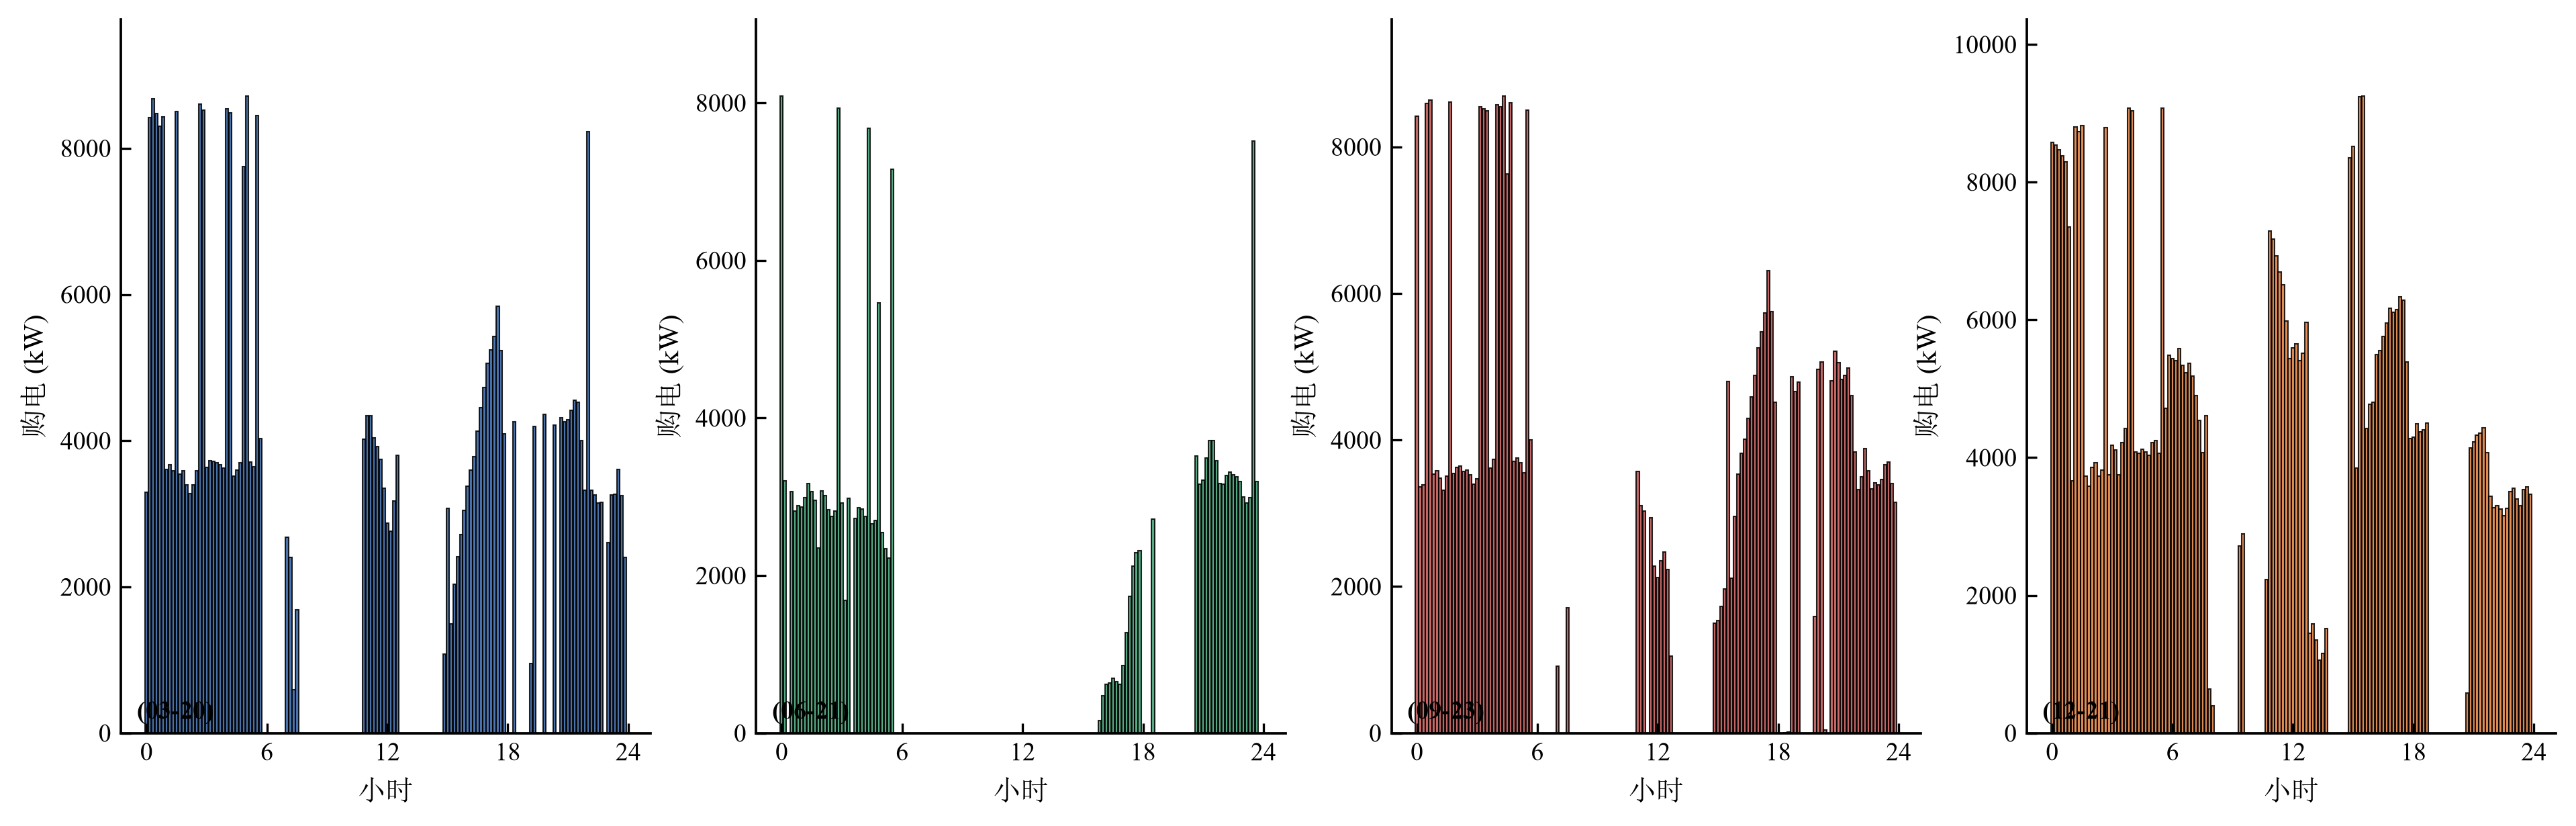
\includegraphics[width=0.75\textwidth]{求解/问题四/图片/图4-2_波动电价四季典型日购电.png}
    \caption{波动电价下四季典型日购电策略}
    \label{fig:结果4-2}
\end{figure}

波动电价下典型日的计划购电与滚动调整购电对比如图\ref{fig:结果4-3}所示。调整策略依然能够在光伏预报更新的时点及时修正购电功率，但由于电价本身波动，调整幅度与固定电价情形存在差异，总体上仍以减小供电缺口、降低高价时段购电为目标。

\begin{figure}[H]
    \centering
    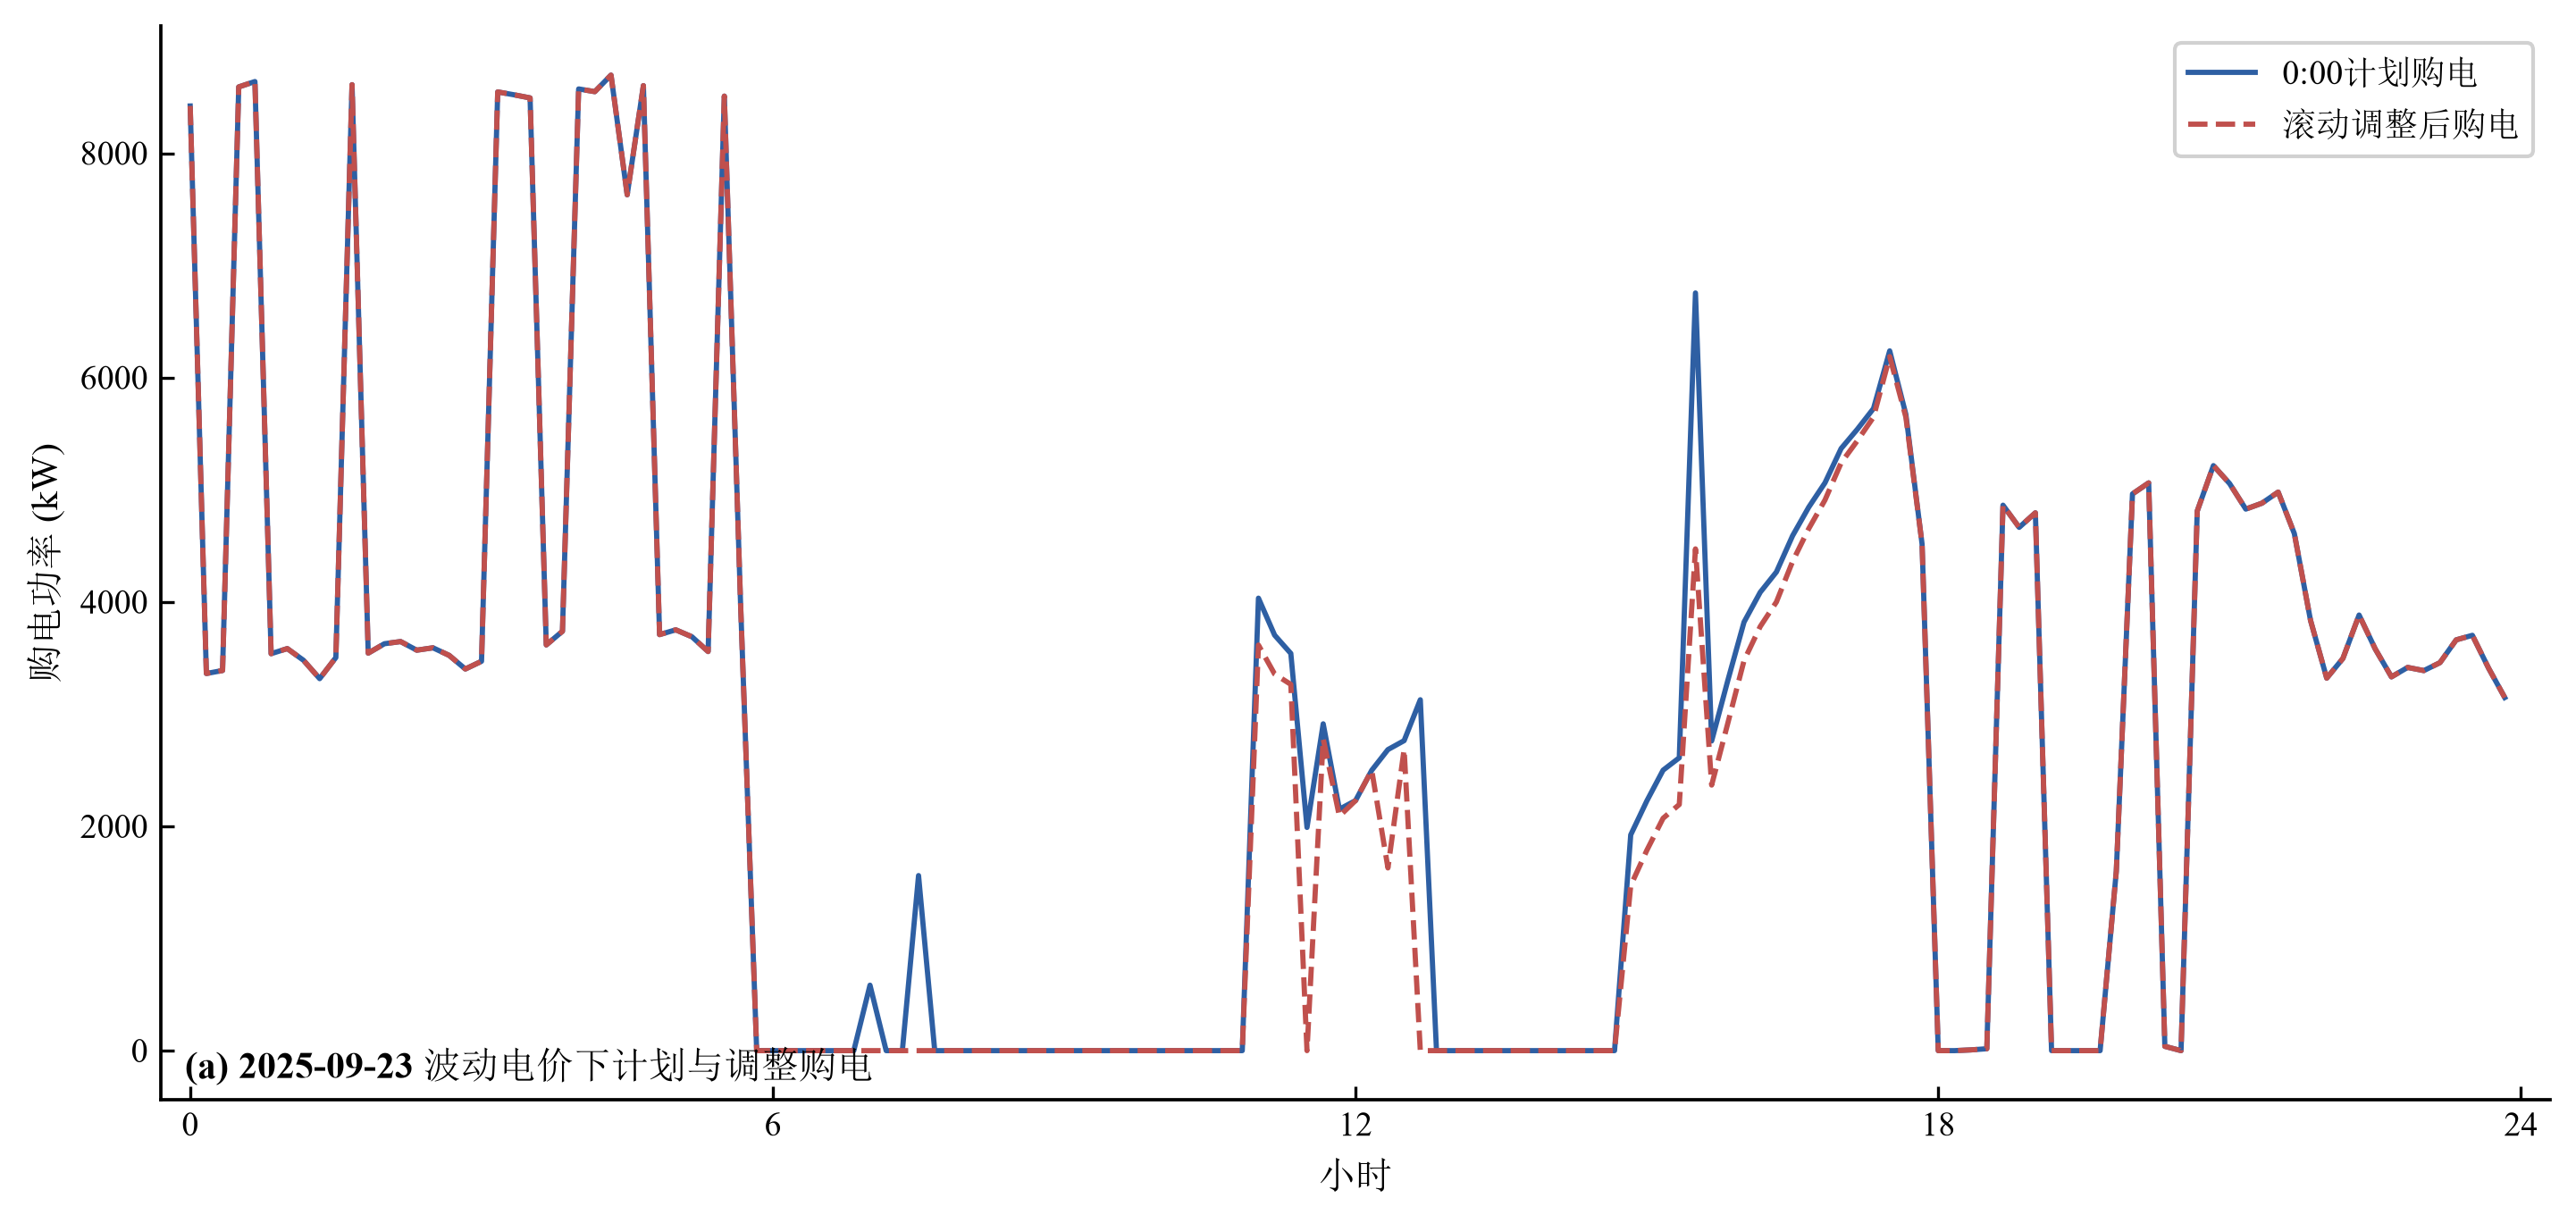
\includegraphics[width=0.70\textwidth]{求解/问题四/图片/图4-3_波动电价滚动调整购电.png}
    \caption{波动电价下典型日计划与调整购电对比}
    \label{fig:结果4-3}
\end{figure}

波动电价下典型日的储能荷电状态轨迹如图\ref{fig:结果4-4}所示。储能荷电状态在一天内完成多次充放切换，以适应波动电价的峰谷变化，且全程满足容量约束，说明储能能够有效利用波动电价的峰谷价差获取套利收益。

\begin{figure}[H]
    \centering
    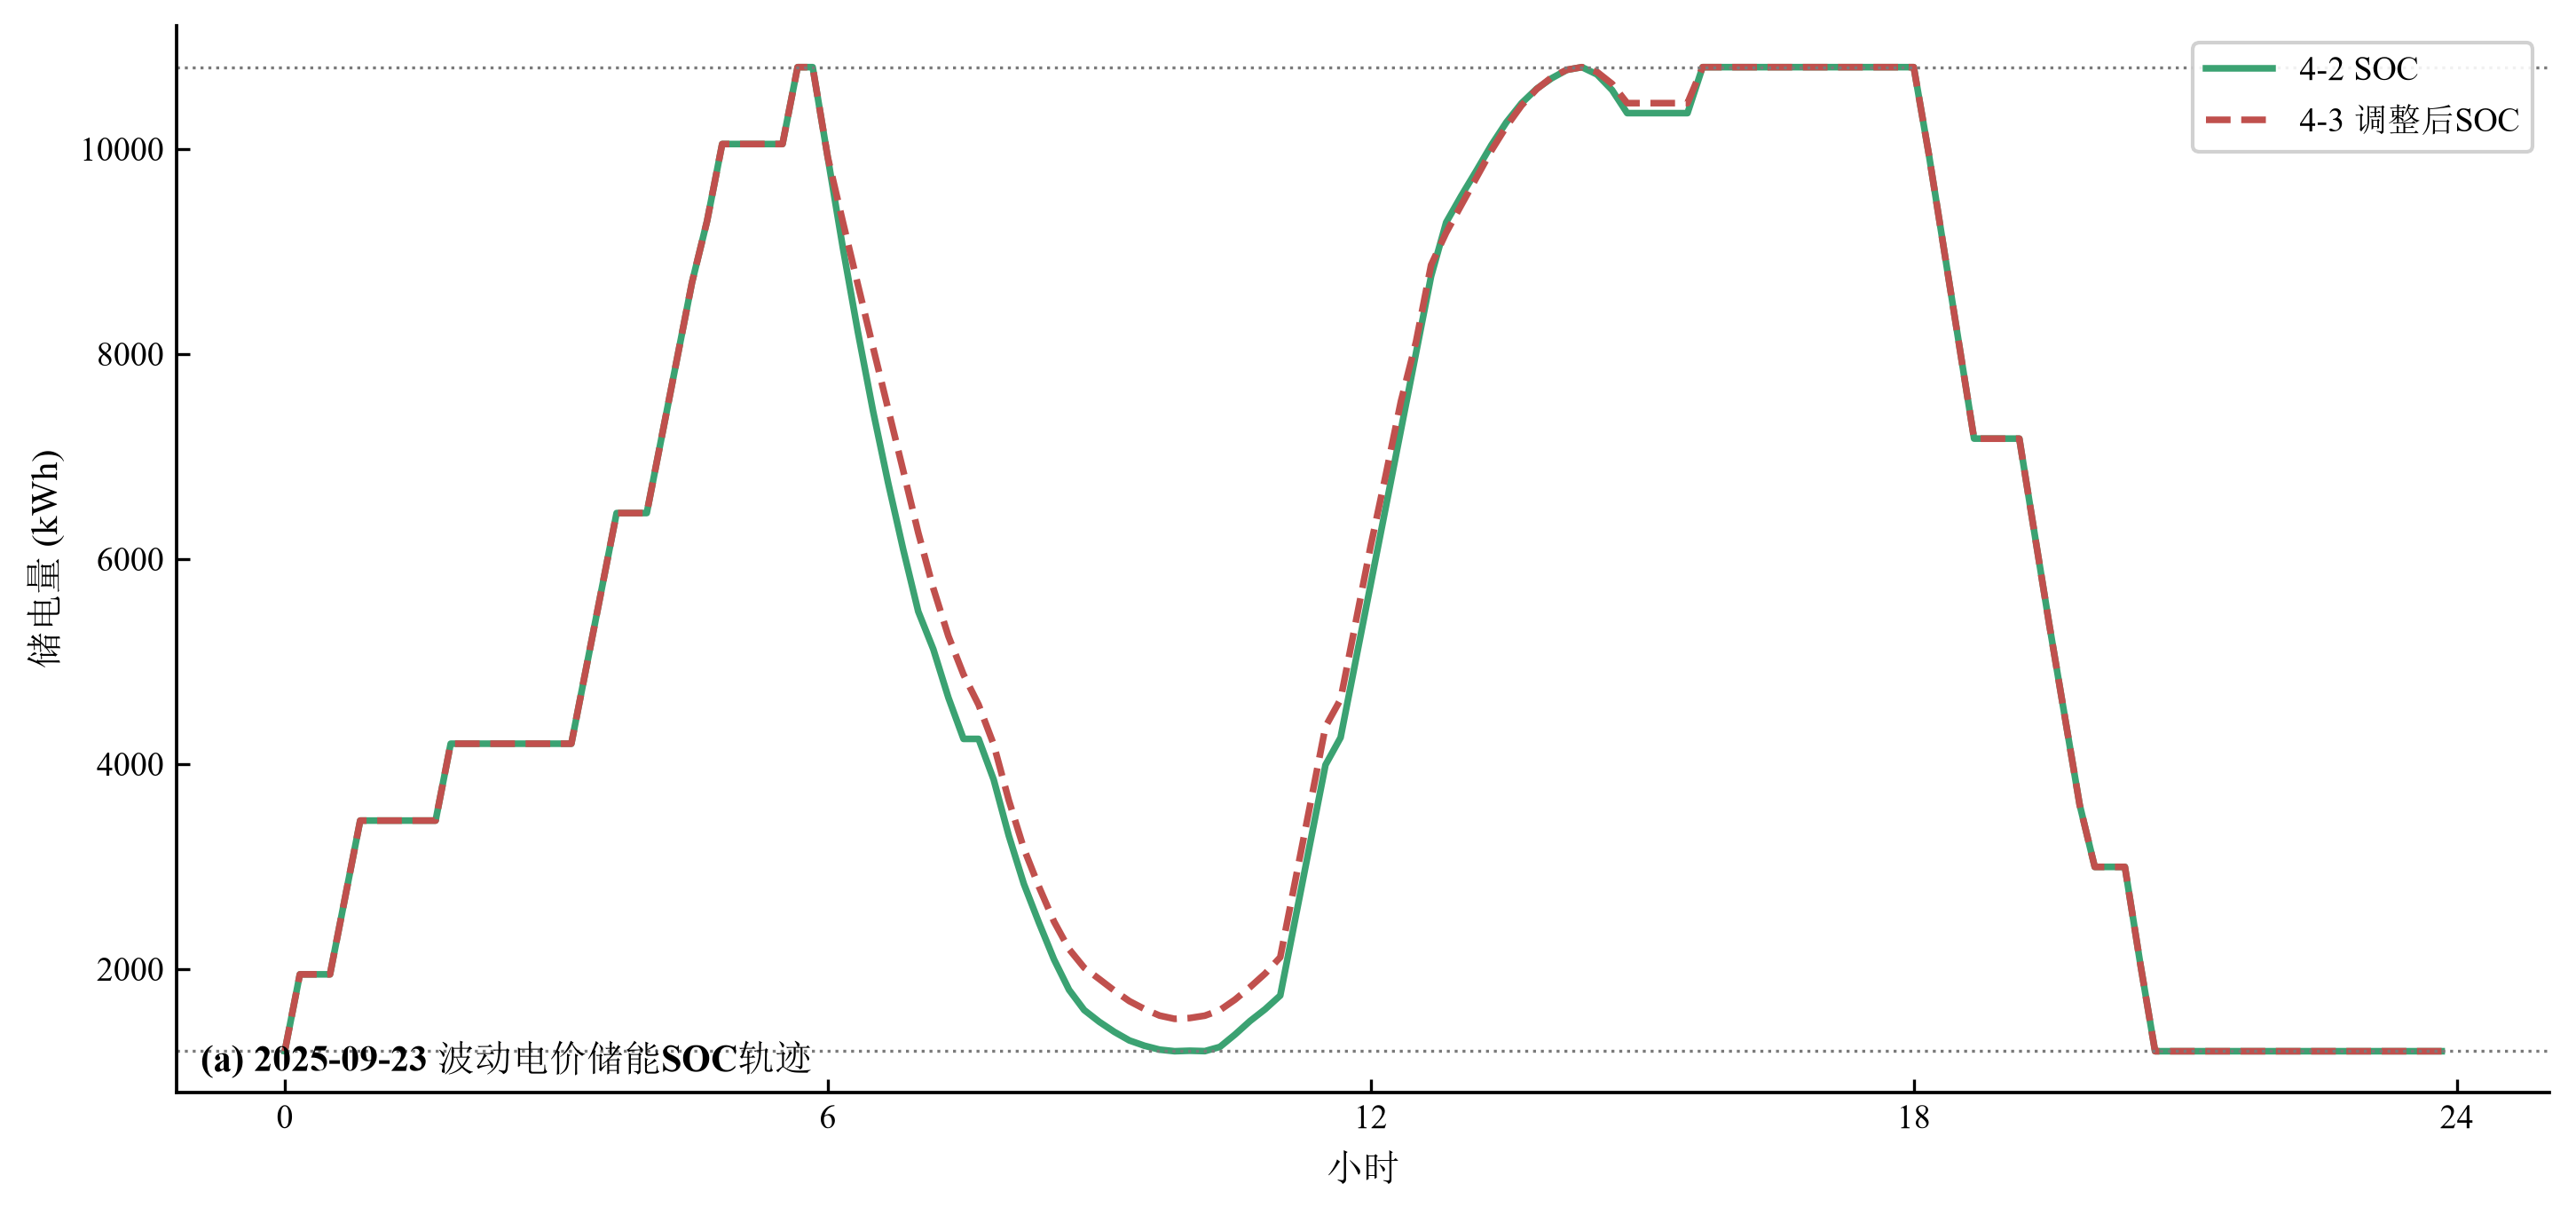
\includegraphics[width=0.70\textwidth]{求解/问题四/图片/图4-4_波动电价SOC轨迹.png}
    \caption{波动电价下典型日储能荷电状态轨迹}
    \label{fig:结果4-4}
\end{figure}

波动电价下 2.1—12.31 逐日紧急购电量如图\ref{fig:结果4-5}所示。紧急购电量整体保持低位，仅在个别预报偏差较大日期出现尖峰，与固定电价情形的规律一致，说明滚动调整在波动电价下同样有效。

\begin{figure}[H]
    \centering
    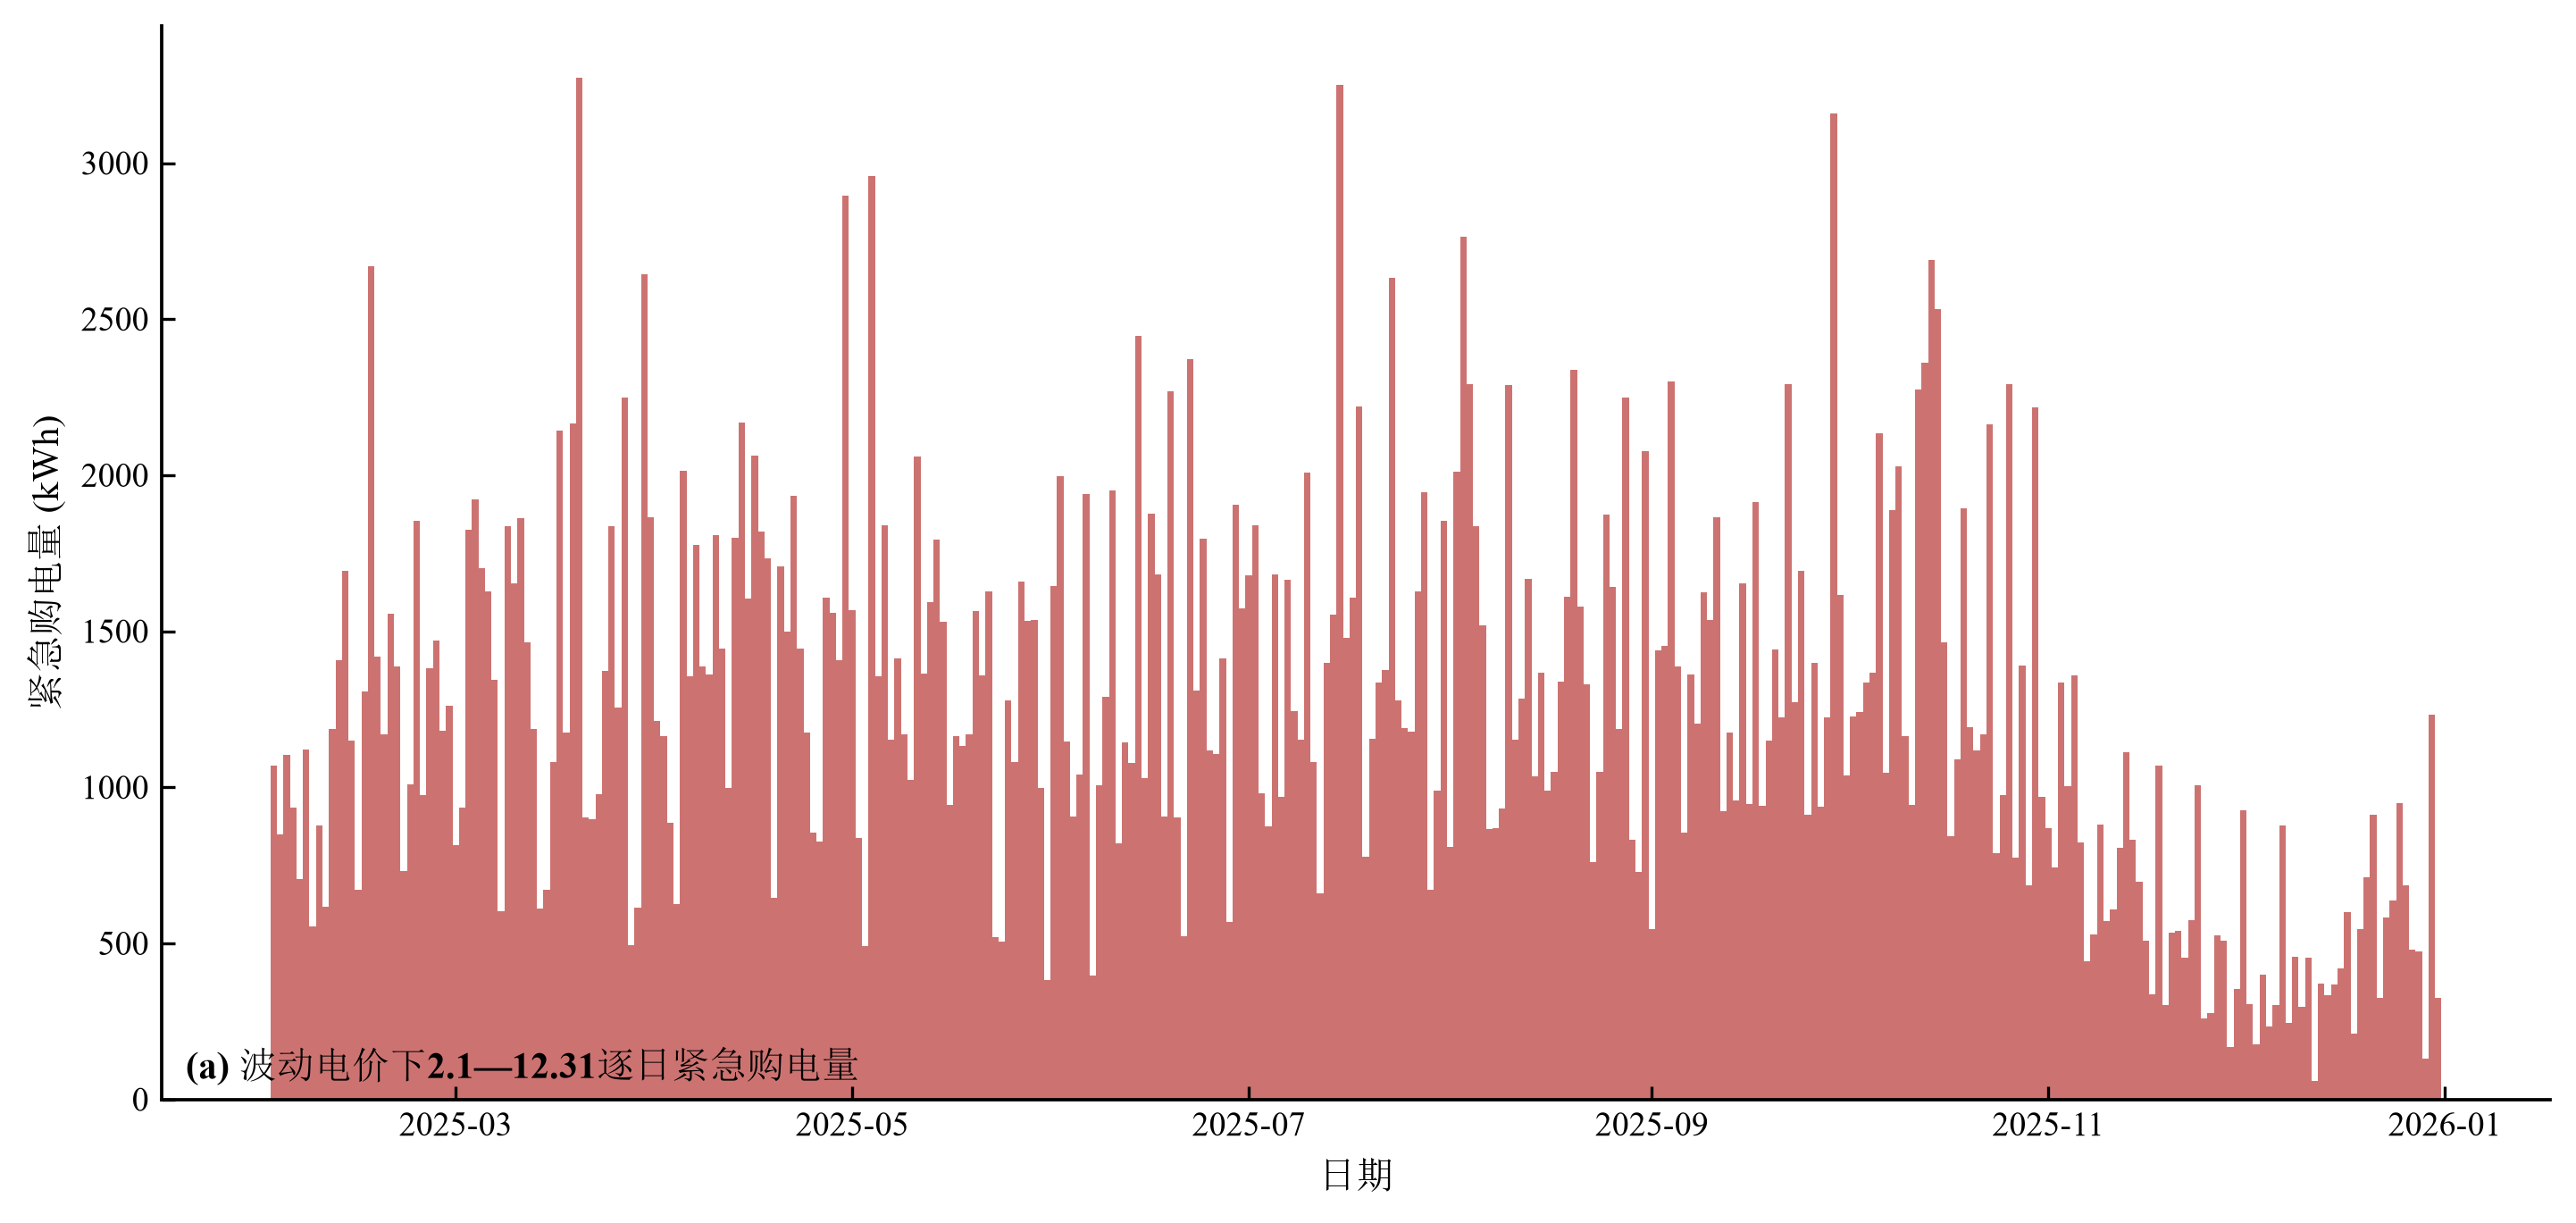
\includegraphics[width=0.70\textwidth]{求解/问题四/图片/图4-5_波动电价紧急购电量.png}
    \caption{波动电价下2.1—12.31逐日紧急购电量}
    \label{fig:结果4-5}
\end{figure}

固定电价与波动电价下的费用对比如图\ref{fig:结果4-6}所示。波动电价下问题二与问题三的费用均高于固定电价情形，其中问题二由 12254765.72 元升至 12841054.36 元，问题三由 14337999.15 元升至 14956526.18 元，说明实时波动的电价增加了微网购电的不确定性与成本，储能套利只能部分对冲电价波动的影响。

\begin{figure}[H]
    \centering
    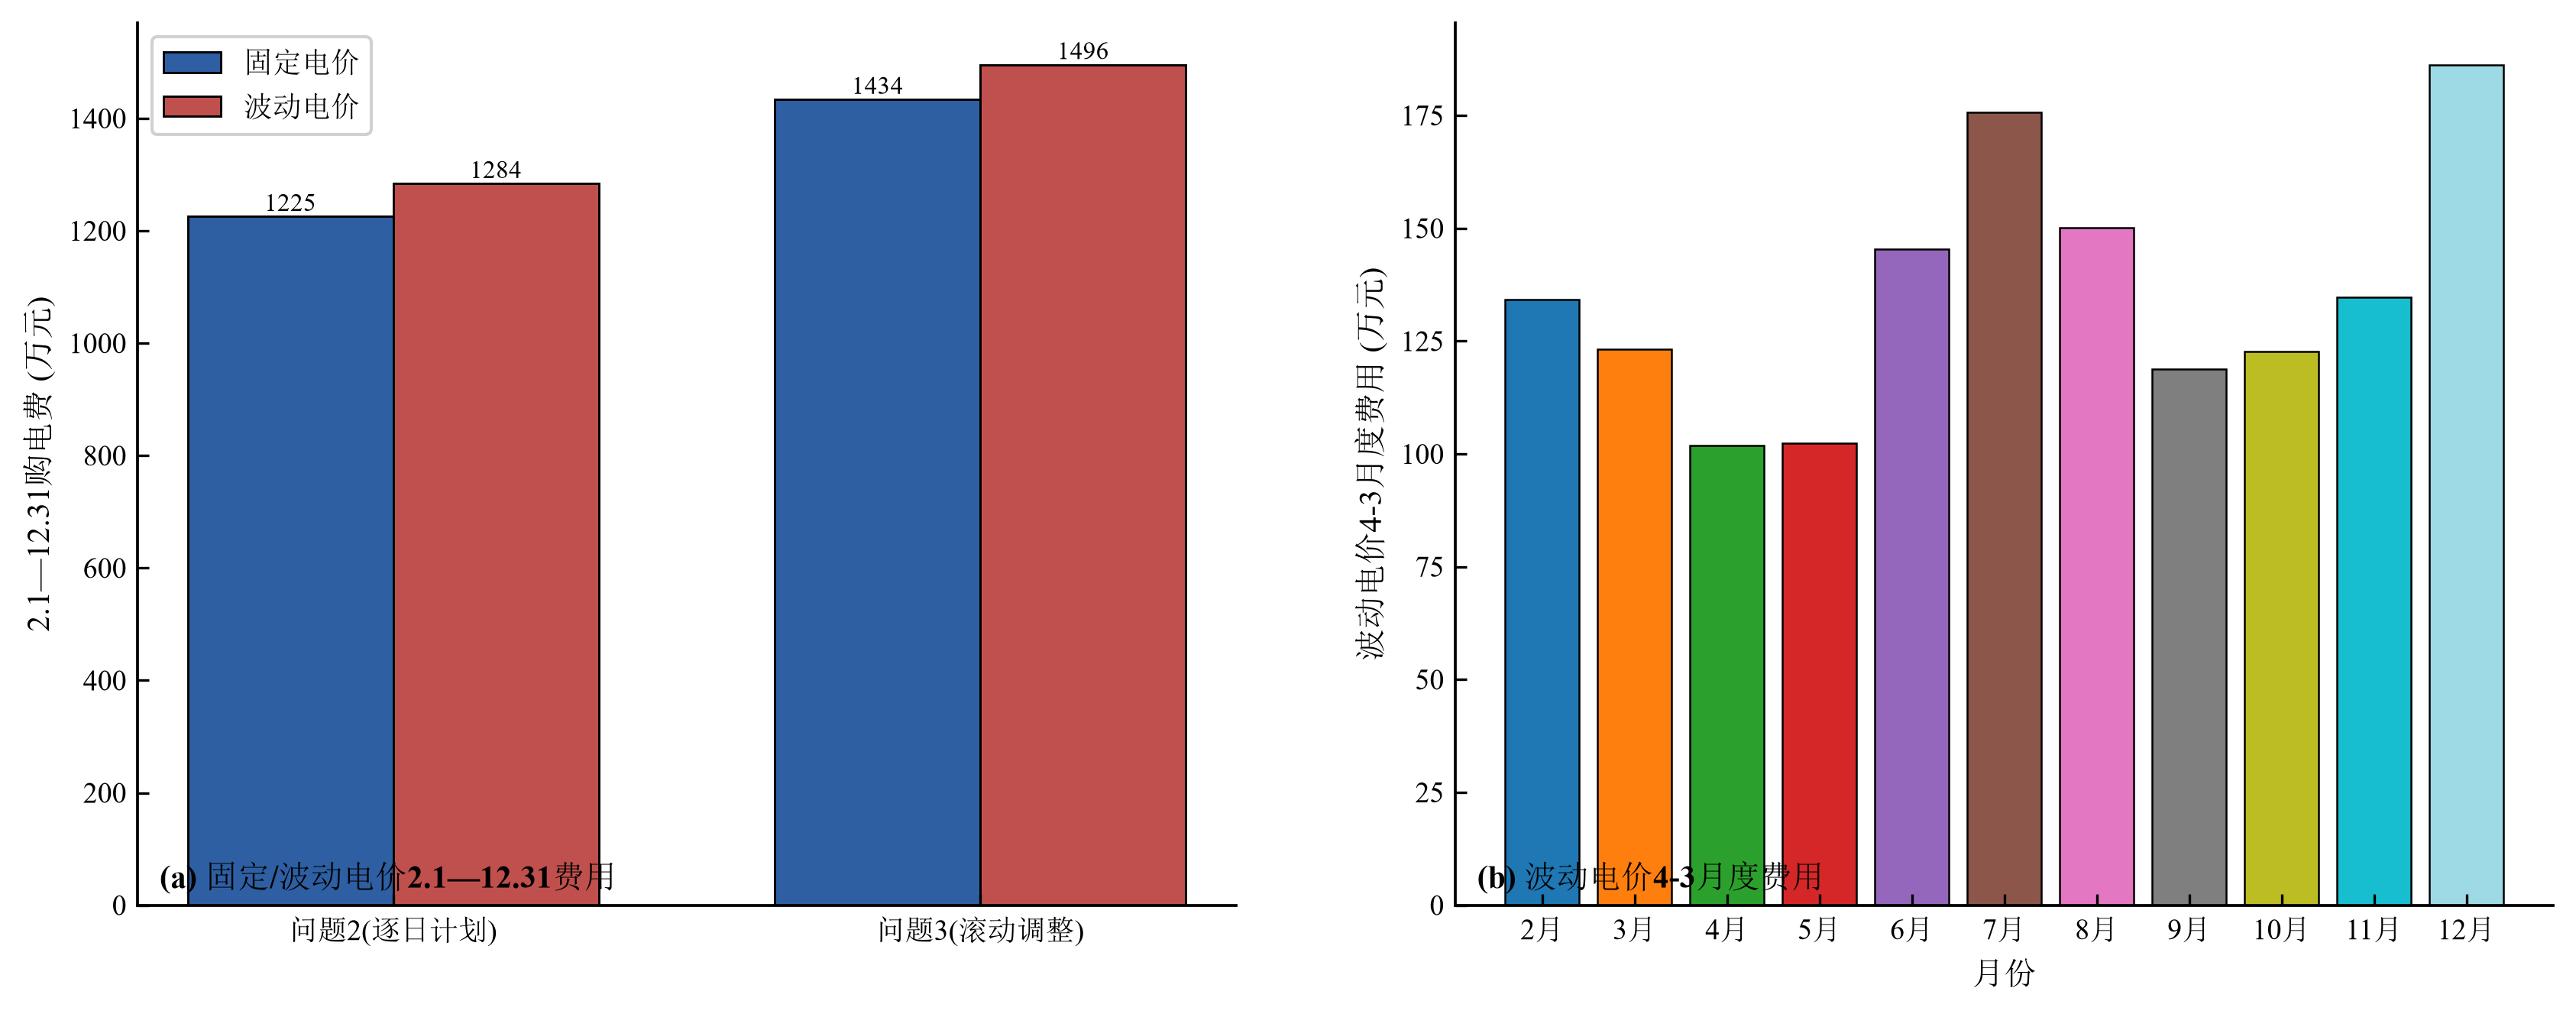
\includegraphics[width=0.72\textwidth]{求解/问题四/图片/图4-6_固定与波动电价费用对比.png}
    \caption{固定电价与波动电价费用对比（2.1—12.31）}
    \label{fig:结果4-6}
\end{figure}

综合以上结果，问题四在波动电价下重新计算了问题二与问题三的购电策略，两套模型均能稳定运行，储能低充高放的套利行为在波动电价下更为活跃，但购电费用较固定电价情形有所上升，结论合理可靠。




% ┈┈┈┈┈┈┈┈┈┈┈┈┈┈┈┈┈┈┈┈┈┈┈┈┈┈┈┈┈┈┈┈┈┈┈
% 【本章节写作提示词】
% ════════════════════════════════════════════
% 【结构】本文件是一级标题「模型的建立与求解」的包装：\section{模型的建立与求解}，内部由下方「__SUBS__ 占位」注入
%   其「子块（二级标题）」的 \input 列表，子块来自 subs/ 下（如 5.1问题1的建立求解、5.2问题2的建立求解…）。
% 【生成】按题目小问数 N 选择 subs/ 下的子块并在组成里排序：N 问就 \input 5.1~5.N；N>4 新建，N<4 删除多余。
% 【每问骨架】每个 5.X.问题X的建立求解 用 \subsection{问题X的模型的建立和求解}，内部再 \input 四个三级子块，顺序固定为：
%   ① 具体分析（问题类型+方法+步骤+流程图）→ ② 模型准备（数据预处理+算法选择）→ ③ 模型建立（分题型建模）→ ④ 模型求解（结果表/图）。组合题型按题目主要类型选择，不必全部选。
% 【图片来源】论文用 求解/问题X/图片/xxx.png 引用；数据用 求解/问题X/结果/ 的 CSV。
% ════════════════════════════════════════════


% ════════════════════════════════════════
% 模型检验与分析（06.模型检验.tex）
% ════════════════════════════════════════
\section{模型检验与分析}

为验证本文构建的模型的有效性和稳健性，进行以下检验。本文模型为线性规划优化模型，其最优性由求解器严格保证\cite{boyd2004}，因此检验重点在于约束满足程度、能量守恒精度与参数灵敏度。

\subsection{误差分析}

对问题一的最优解逐项核验其约束满足情况与能量守恒精度，结果如表\ref{tab:error}所示。

\begin{longtable}{>{\centering\arraybackslash}p{0.30\textwidth}>{\centering\arraybackslash}p{0.26\textwidth}>{\raggedright\arraybackslash}p{0.36\textwidth}}
  \caption{模型误差分析结果}
  \label{tab:error} \\
  \toprule
  检验项 & 检验结果 & 说明 \\
  \midrule
  \endfirsthead
  \caption{模型误差分析结果（续）} \\
  \toprule
  检验项 & 检验结果 & 说明 \\
  \midrule
  \endhead
  \bottomrule
  \endfoot
  功率平衡最大残差 & $1.36\times10^{-12}$ & 能量守恒严格满足 \\
  储电量越界次数 & 0 & 全程处于 $[1200,10800]$ kWh \\
  充放电功率越界次数 & 0 & 始终不超过 5000 kW \\
  储电初值约束 & 满足 & $E_0=6000$ kWh，与附录1给定一致 \\
  日循环约束残差 & 0 & $E_0=E_{144}=6000$ kWh \\
\end{longtable}

如表\ref{tab:error}所示，最优解的功率平衡残差处于 $10^{-12}$ 量级，储能荷电状态与充放电功率全程处于约束区间，日循环约束严格成立，验证了模型求解的正确性与数值精度。

\subsection{灵敏度分析}

为检验模型对关键参数的稳健性，分别调整储能充放电效率、最大充放电功率、储电量下限与负荷水平，观察全天购电费的变化，结果如表\ref{tab:sensitivity}所示。

\begin{longtable}{>{\centering\arraybackslash}p{0.30\textwidth}>{\centering\arraybackslash}p{0.30\textwidth}>{\raggedright\arraybackslash}p{0.32\textwidth}}
  \caption{灵敏度分析结果}
  \label{tab:sensitivity} \\
  \toprule
  参数变化 & 输出变化 & 灵敏度评估 \\
  \midrule
  \endfirsthead
  \caption{灵敏度分析结果（续）} \\
  \toprule
  参数变化 & 输出变化 & 灵敏度评估 \\
  \midrule
  \endhead
  \bottomrule
  \endfoot
  $\eta=0.85$ & 36603.41 元 & 费用上升 4.20\% \\
  $\eta=0.95$ & 33767.03 元 & 费用下降 3.87\% \\
  $P_{\max}=4000$ & 35247.87 元 & 费用上升 0.34\% \\
  $P_{\max}=6000$ & 35083.29 元 & 费用下降 0.12\% \\
  $E_{\min}=1500$ & 35329.91 元 & 费用上升 0.58\% \\
  负荷 $+5\%$ & 38834.17 元 & 费用上升 10.55\% \\
  负荷 $-5\%$ & 31552.18 元 & 费用下降 10.18\% \\
\end{longtable}

如表\ref{tab:sensitivity}所示，购电费对充放电效率最为敏感，效率每提高 5\% 可使费用下降约 4\%，说明储能效率是影响经济性的关键因素；充放电功率与储电量下限的小幅变化对费用的影响均不足 1\%，模型稳健；负荷水平按比例影响费用，符合能量平衡的线性规律。综上，模型在各参数摄动下均表现稳定，结果可靠。


% ════════════════════════════════════════
% 模型的评价（07.模型评价.tex）
% ════════════════════════════════════════
\section{模型的评价}

\subsection{模型的优点}
\begin{itemize}[itemindent=2em]
\item \textbf{优点1：}线性规划模型结构简洁、约束刻画完整，所有决策变量均为连续变量，求解器可严格保证全局最优，避免了启发式算法陷入局部最优的风险。
\item \textbf{优点2：}滚动调整模型利用上境变量将分段惩罚费用精确线性化，在不引入整数变量的前提下完整刻画违约与超额的经济代价，计算效率高。
\item \textbf{优点3：}逐日滚动与储电量传递机制将全年大规模优化分解为数百个日尺度小问题，既降低了计算复杂度，又保持了全年储电量的连续性。
\item \textbf{优点4：}模型具有高度可迁移性，只需替换电价、负载与光伏序列即可适应不同季节、不同地区乃至波动电价场景，并通过灵敏度分析验证了稳健性。
\end{itemize}

\subsection{模型的缺点}
\begin{itemize}[itemindent=2em]
\item \textbf{缺点1：}模型假设各 10 分钟间隔内功率恒定，忽略了更短时间尺度上的功率波动对储能实际运行的影响。
\item \textbf{缺点2：}滚动调整模型假定负荷完全可预知、储能严格按计划执行，未考虑储能动态响应光伏实时偏差的闭环控制过程。
\end{itemize}


% ════════════════════════════════════════
% 模型的改进与推广（08.模型改进推广.tex）
% ════════════════════════════════════════
\section{模型的改进与推广}

\subsection{模型的改进}

本文模型的不足主要体现在三个方面。在方法层面，可将光伏预报误差建模为随机变量，引入两阶段随机规划或鲁棒优化，在目标函数中显式权衡期望购电费用与违约风险，使调整策略更具前瞻性。在参数层面，可将储能充放电效率进一步细分为充电效率与放电效率、考虑电池循环寿命损耗与自放电率，并引入储电量分段折旧成本，使经济模型更贴近实际设备。在数据层面，可结合历史气象数据与数值天气预报，对光伏预报误差的分布进行估计，据此优化各预报时刻的储能安全裕度，进一步降低紧急购电费用。

\subsection{模型的推广}

本文建立的微网购电与储能调控模型具有较强的通用性，可直接推广到更广泛的工程与政策场景。在工程领域，该模型可用于工业园区、商业综合体与电动汽车充电站的储能容量配置与日前调度，也可嵌入虚拟电厂的能量管理系统，实现多主体分布式资源的协同优化；在政策领域，该模型可用于评估分时电价、尖峰电价等价格机制的引导效果，为需求响应与储能补贴政策的制定提供量化依据；在行业领域，其滚动调整与惩罚机制思想可迁移到电力现货市场交易、天然气购销合同与物流库存管理等存在预测更新与违约成本的场景，具有广泛的适用价值。


% ════════════════════════════════════════
% AI工具使用声明（09.AI说明.tex）
% ════════════════════════════════════════
\newpage
\section*{AI工具使用声明}


本参赛队在竞赛过程中使用了AI工具，主要用于代码编写与调试、数据处理的辅助实现以及论文文字的语言润色，详细使用情况见支撑材料。


% ════════════════════════════════════════
% 参考文献（10.参考文献.tex）
% ════════════════════════════════════════
\newpage
\begin{thebibliography}{99}

\bibitem{lasseter2002} Lasseter R H. Microgrids[C]//IEEE Power Engineering Society Winter Meeting. New York: IEEE, 2002: 305-308.
\bibitem{kanchev2011} Kanchev H, Lu D, Colas F, et al. Energy management and operational planning of a microgrid with a PV-based active generator for smart grid applications[J]. IEEE Transactions on Industrial Electronics, 2011, 58(10): 4583-4592.
\bibitem{dantzig1963} Dantzig G B. Linear programming and extensions[M]. Princeton: Princeton University Press, 1963.
\bibitem{boyd2004} Boyd S, Vandenberghe L. Convex optimization[M]. Cambridge: Cambridge University Press, 2004.
\bibitem{parisio2014} Parisio A, Rikos E, Glielmo L. A model predictive control approach to microgrid operation optimization[J]. IEEE Transactions on Control Systems Technology, 2014, 22(5): 1813-1827.
\bibitem{rawlings2017} Rawlings J B, Mayne D Q, Diehl M. Model predictive control: theory, computation, and design[M]. 2nd ed. Santa Barbara: Nob Hill Publishing, 2017.
\bibitem{antonanzas2016} Antonanzas J, Osorio N, Escobar R, et al. Review of photovoltaic power forecasting[J]. Solar Energy, 2016, 136: 78-111.
\bibitem{sioshansi2010} Sioshansi R, Denholm P, Jenkin T, et al. Estimating the value of electricity storage in PJM: arbitrage and some welfare effects[J]. Energy Economics, 2010, 31(2): 269-277.
\bibitem{camacho2013} Camacho E F, Bordons C. Model predictive control[M]. 2nd ed. London: Springer, 2013.
\bibitem{si2009} 司守奎, 孙玺菁. 数学建模算法与应用[M]. 北京: 国防工业出版社, 2011.

\end{thebibliography}


% ════════════════════════════════════════
% 附录（11.附录.tex）
% ════════════════════════════════════════
\newpage
\makeatletter
\let\@oldaddcontentsline\addcontentsline
\renewcommand{\addcontentsline}[3]{}

\section*{附录}
\let\addcontentsline\@oldaddcontentsline
\makeatother

\renewcommand{\arraystretch}{1.2}
\begin{longtable}{>{\centering\arraybackslash}p{0.34\textwidth}>{\raggedright\arraybackslash}p{0.62\textwidth}}
  \caption{附件说明表}
  \label{tab:appendix} \\
  \toprule
  文件 & 说明 \\
  \midrule
  \endfirsthead
  \caption{附件说明表（续）} \\
  \toprule
  文件 & 说明 \\
  \midrule
  \endhead
  \bottomrule
  \endfoot
  求解/问题一/问题一.py & 问题一单日计划购电线性规划求解代码 \\
  求解/问题二/问题二.py & 问题二全年逐日滚动购电求解代码 \\
  求解/问题三/问题三.py & 问题三滚动预报调整购电求解代码 \\
  求解/问题四/问题四.py & 问题四波动电价重算求解代码 \\
  求解/\_models.py & 线性规划建模与数据读取公共模块 \\
  求解/问题X/图片/ & 各问题结果图（共 24 幅） \\
  数据/result1.xlsx & 问题一完整计划购电策略结果文件 \\
  数据/result2.xlsx & 问题二完整购电策略结果文件 \\
  数据/result3.xlsx & 问题三完整购电策略结果文件 \\
  数据/result4-2.xlsx & 问题四波动电价下问题二结果文件 \\
  数据/result4-3.xlsx & 问题四波动电价下问题三结果文件 \\
\end{longtable}


\end{document}
